%%%%%%%%%%%%%%%%%%%%%%%%%%%%%%%%%%%%%%%%%%%%%%%%%%%
%
%  New template code for TAMU Theses and Dissertations starting Fall 2012.  
%  For more info about this template or the 
%  TAMU LaTeX User's Group, see http://www.howdy.me/.
%
%  Author: Wendy Lynn Turner 
%	 Version 1.0 
%  Last updated 8/5/2012
%
%%%%%%%%%%%%%%%%%%%%%%%%%%%%%%%%%%%%%%%%%%%%%%%%%%%
%%%                           SECTION V
%%%%%%%%%%%%%%%%%%%%%%%%%%%%%%%%%%%%%%%%%%%%%%%%%%%
\chapter{\uppercase {FEM Basis Functions for Unstructured Polytopes}}
\label{sec::BF}


In Section \ref{sec::Sn_Spatial}, we detailed the spatial discretization of the transport equation. We then proceeded to give the functional forms for the various elementary matrices needed to form the full set of spatially-discretized PDEs. These included the mass, streaming, and surface matrices where the integrations on the element's domain and boundary require combinations of the basis functions' values and gradients. From FEM theory \cite{ern2013theory}, the basis functions act as interpolation functions with local measure on some subset of elements on a discretized mesh, $\mathbb{T}_h$. To achieve the maximum possible solution convergence rate for regular solutions of $p+1$, the basis functions must have polynomial completeness of at least order $p$. For 2D interpolants, the basis functions are linearly-complete ($p=1$) if they can exactly interpolate the $\{ 1, x, y \}$ span of functions. Likewise, 2D basis functions are said to be quadratically-complete if they can exactly interpolate the $\{ 1, x, y, x^2, xy, y^2 \}$ span of functions. This work seeks to analyze the use of the different linearly-complete polygonal basis functions with the DGFEM $S_N$ transport equation. We then seek to extend this analysis to quadratically-complete basis functions, thus achieving higher convergence rates (third-order). We will do this by utilizing the methodology developed by Rand et al. \cite{rand2014quadratic} on the different linearly-complete polygonal coordinates.

The remainder of this chapter is organized as follows. In Section \ref{sec::BF_2DLinear}, we present the 2D, linearly-complete, barycentric, polygonal basis functions that we will analyze in this dissertation. We then present in Section \ref{sec::BF_2DQuadratic} the methodology to convert the barycentric polygonal basis functions presented in Section \ref{sec::BF_2DLinear} into a serendipity space of basis functions with quadratic-completeness. Section \ref{sec::BF_2DIntegration} provides the methodology that will be employed to generate spatial quadrature sets on 2D arbitrary polygons. Section \ref{sec::BF_3DLinear} then presents the 3D, linearly-complete, polyhedral basis functions that will be exclusively used in Chapter \ref{sec::DSA} for 3D DSA calculations. We then present numerical results pertaining to our linear and quadratic 2D basis functions in Section \ref{sec::BF_Results}. Section \ref{sec::BF_Conclusions} concludes with some closing remarks.

%%%%%%%%%%%%%%%%%%%%%%%%%%%%%%%%%%%%%%%%%%%%%%%%%%%
%%%   Section - 2D Linear
\section{Linear Basis Functions on 2D Polygons}
\label{sec::BF_2DLinear}

Figure \ref{fig::BF_2D_ref_polygon}, gives an image of a reference polygon along with the geometric notations we will use to define the different linear polygonal coordinates. An element, $K\in \mathbb{R}^2$, is defined by a closed set of $N_K$ points (vertices) in $\mathbb{R}^2$. The vertices are ordered ($1,...,N_K$) in a counter-clockwise manner without restriction on their convexity. Face $j$ on the polygon, $e_j$, is defined as the line segment between vertices $j$ and $j+1$. The vertex $j+1$ is determined in general as $j+1 =\mod(j,N_K)+1$, which gives a wrap-around definition of vertex $N_K+1 = 1$.

\begin{figure}
\centering
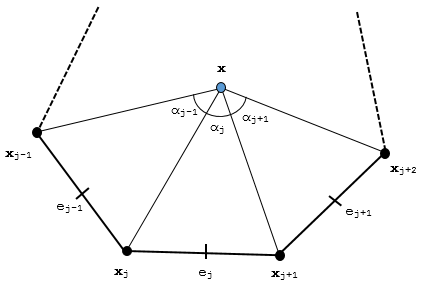
\includegraphics[width=0.85\textwidth]{figures/sec_BF/ref_polygon_Rev1.png}
\caption{Arbitrary polygon with geometric properties used for 2D basis function generation.}
\label{fig::BF_2D_ref_polygon}
\end{figure}

We complete our geometric description for the polygonal coordinate system by analyzing a point $\vec{x}$ inside the polygon's domain, as also seen in Figure \ref{fig::BF_2D_ref_polygon}. $\alpha_j$ is the angle between the points ($\vec{x}_j, \vec{x}, \vec{x}_{j+1}$).We conclude by defining $|\vec{u}|$ as the Euclidean distance of the vector $\vec{u}$. This means that $|\vec{x} - \vec{x}_j|$ is the distance between the points $\vec{x}$ and $\vec{x}_j$ and $|e_j|$ is the length of face $j$ between points $\vec{x}_j$ and $\vec{x}_{j+1}$.


In this dissertation, all linearly-complete, 2D basis functions for an element $K$ will obey the properties for barycentric coordinates. If the element $K$ is composed of $N_K$ vertices, then it contains $N_K$ barycentric coordinates, where each one is located at a vertex. These barycentric coordinates will form a {\em partition of unity},

\begin{equation}
\sum_{j=1}^{N_K} b_j (\vec{x})  =  1;
\label{eq::BF_linear_interp_partition}
\end{equation}

\noindent coordinate interpolation will result from an {\em affine combination} of the vertices,

\begin{equation}
\sum_{j=1}^{N_K} b_j (\vec{x}) \vec{x}_j  =  \vec{x};
\label{eq::BF_linear_interp_affine}
\end{equation}

\noindent and they will satisfy the {\em Lagrange property},

\begin{equation}
b_j (\vec{x}_i) = \delta_{ij}.
\label{eq::BF_linear_interp_lagrange}
\end{equation}

\noindent They also have piecewise linearity on faces adjacent to their vertex. As an example of this, consider the function at vertex $j$, $b_j$, along face $e_j$. Then the piecewise linearity of the function on the face means that it can interpolate as

\begin{equation}
\label{eq::BF_linear_bound_interp}
b_j ((1-\mu ) \vec{x}_j  + \mu \vec{x}_{j+1})  = (1-\mu ) b_j (\vec{x}_j ) + \mu b_j (\vec{x}_{j+1} ) , \qquad \mu \in [0,1].
\end{equation}

Using the {\em partition of unity} of Eq. (\ref{eq::BF_linear_interp_partition}), we can rewrite Eqs. (\ref{eq::BF_linear_interp_partition}-\ref{eq::BF_linear_interp_affine}) into a separate, compact, vectorized form for completeness

\begin{equation}
\sum_{j=1}^{N_K}  b_j (\vec{x}) \vec{c}_{j,1}(\vec{x}) = \vec{q}_1 ,
\label{eq::BF_linear_interp_req_vector}
\end{equation}

\noindent where $\vec{c}_{j,1}(\vec{x})$ and $\vec{q}_1$ are the linearly-complete constraint and equivalence terms, respectively. These terms are simply:

\begin{equation}
\vec{c}_{j,1}(\vec{x}) = \left[
\begin{array}{c}
1 \\
x_j - x \\
y_j - y
\end{array} \right]
  \qquad \text{and} \qquad \vec{q}_1 = \left[
\begin{array}{c}
1 \\
0 \\
0
\end{array} \right],
\label{eq::BF_linear_constraint_terms}
\end{equation}

\noindent respectively. Equation (\ref{eq::BF_linear_interp_req_vector}) states that our interpolation functions (the basis functions) can exactly reproduce polynomial functions up to order 1. This is why we state that our basis functions are linearly-complete. However, we will not restrict our $N_K$ basis functions to be polynomials. In fact, of the basis functions that we will use, only the PWL coordinates are formed by combinations of polynomial functions.


%%%%%%%%%%%%%%%%%%%%%%%%%%%%%%%%%%%%%%%%%%%%%%%%%%%
%%%   SubSection - Wachspress
\subsection{Wachspress Rational Basis Functions}
\label{sec::BF_2DLinear_Wachspress}

The first linearly-complete polygonal coordinates that we will consider are the Wachspress rational functions \cite{wachspress1975rational}. These rational functions were the first derived for 2D polygons and possess all the properties of the barycentric coordinates previously detailed. However, they are only valid interpolants over strictly-convex polygons. They have zero measure and blow up for weakly-convex and concave polygons, respectively. Also, their values and gradients cannot be directly evaluated on the polygonal boundary. However, they do have a valid limit which we show in Appendix \ref{sec::appendix_BF}. The Wachspress coordinates (which we denote as $b^W$) have the following form

\begin{equation}
\label{eq::BF_wach_BF}
b_{j}^{W} (\vec{x}) = \frac{w_j (\vec{x}) }{\sum\limits_{i=1}^{N_K} w_i (\vec{x})},
\end{equation}

\noindent where the Wachspress weight function for vertex $j$, $w_j$, has the following definition:

\begin{equation}
\label{eq::BF_wach_weights}
w_j (\vec{x})  = \frac{A(\vec{x}_{j-1}, \vec{x}_{j}, \vec{x}_{j+1})}{A(\vec{x}, \vec{x}_{j-1}, \vec{x}_{j}) \, A(\vec{x}, \vec{x}_{j}, \vec{x}_{j+1})} .
\end{equation}

\noindent In Eq. (\ref{eq::BF_wach_weights}), the terms $A(\vec{a}, \vec{b}, \vec{c})$ denote the signed area of the triangle with vertices $\vec{a}$, $\vec{b}$, and $\vec{c}$. Each of these signed areas can be computed by

\begin{equation}
\label{eq::BF_wach_signed_area}
A(\vec{a}, \vec{b}, \vec{c}) = \frac{1}{2}
\left|  
  \begin{array}{ccc}
  1 & 1 & 1 \\
  x_a & x_b & x_c \\
  y_a & y_b & y_c
  \end{array}
\right| .
\end{equation}

There is an alternative method of expressing the Wachspress weight functions. Warren et al. \cite{warren2007barycentric} proposed weight functions that are defined in terms of the perpendicular distance of the point $\vec{x}$ to the polygon's faces. Using the reference polygon of Figure \ref{fig::BF_2D_ref_polygon}, the perpendicular distance of the point $\vec{x}$ to the face $j$ is denoted as $h_j (\vec{x})$ and is given by

\begin{equation}
\label{eq::BF_wach_perp_dist}
h_j (\vec{x}) = \left(  \vec{x}_j - \vec{x} \right) \cdot \vec{n}_j = \left(  \vec{x}_{j+1} - \vec{x} \right) \cdot \vec{n}_j , 
\end{equation}

\noindent where $\vec{n}_j$ is the outward normal direction of face $j$. Using these perpendicular distances, the Wachspress coordinates can be calculated using Eq. (\ref{eq::BF_wach_BF}) with new function definitions of

\begin{equation}
\label{eq::BF_wach_wt_perpdist}
 w_j (\vec{x}) = \frac{\vec{n}_{j-1} \, \times \, \vec{n}_j}{h_{j-1} (\vec{x}) h_j (\vec{x})} ,
\end{equation}

\noindent where

\begin{equation}
\label{eq::BF_wach_cross}
\vec{x}_{1} \times \vec{x}_2 = 
\left|  
\begin{array}{ccc}
x_1 & x_2 \\
y_1 & y_2
\end{array}
\right| .
\end{equation}

For FEM theory, the basis function gradients are also necessary to compute some of the elementary matrices. The gradients of the Wachspress rational functions are straightforward to calculate by simply taking the partial derivatives of Eq. (\ref{eq::BF_wach_BF}). Then, using derivative rules along with some algebra, the Wachspress gradients are given by,

\begin{equation}
\label{eq::BF_wach_gradient}
 \vec{\nabla} b_{j}^{W}(\vec{x}) = b_{j}^{W} (\vec{x}) \left( \vec{R}_j  (\vec{x})- \sum\displaylimits_{i}   b_{i}^{W} (\vec{x}) \vec{R}_i (\vec{x}) \right) ,
\end{equation}

\noindent where the reduced gradient, $\vec{R}_j$, is defined as

\begin{equation}
\label{eq::BF_wach_reduced_grad}
\vec{R}_j (\vec{x})  = \frac{1}{w_j} \vec{\nabla} w_j .
\end{equation}

\noindent This means that the gradients of the Wachspress coordinates can be calculated by combinations of the all the weight functions and their gradients. The weight function gradients are easy to compute using the perpendicular form. The gradient of the $j$ weight functions is given by

\begin{equation}
\label{eq::BF_wach_grad_perpdist}
 \vec{\nabla} w_j (\vec{x}) = w_j (\vec{x})  \left(  \frac{\vec{n}_{j-1}}{h_{j-1} (\vec{x})} + \frac{\vec{n}_{j}}{h_{j} (\vec{x})} \right) .
\end{equation}

\noindent This lets us immediately see that $\vec{R}_j$ is simply

\begin{equation}
\label{eq::BF_wach_reduce_grad_form}
\vec{R}_j (\vec{x})  = \frac{\vec{n}_{j-1}}{h_{j-1} (\vec{x})} + \frac{\vec{n}_{j}}{h_{j} (\vec{x})}.
\end{equation}

We now give a pair of contour plots of the Wachspress coordinates. First, Figure \ref{fig::2D_WACHSPRESS1_unit_square_basis_functions} provides the contour plots of the four Wachspress functions on the unit square. We see that the functions are smoothly varying within the square with at least $C^1$ continuity. Then in Figure \ref{fig::2D_WACHSPRESS1_deg_square_basis_functions}, we give the contour plots for a degenerate pentagon which is simply the unit square with a vertex added at point ($1/2,1$). We see how the functions fail for this weakly-convex case. The function located at the degenerate vertex has zero measure everywhere within the polygon. Also, the functions located at the vertices adjacent to the degenerate vertex no longer maintain linearity on their adjacent faces. We will not show it here for brevity, but the Wachspress functions on concave polygons will have points in the interior that will result in divide-by-zero operations.

\begin{figure}
\centering
	\begin{subfigure}[b]{0.39\textwidth}
		\centering
		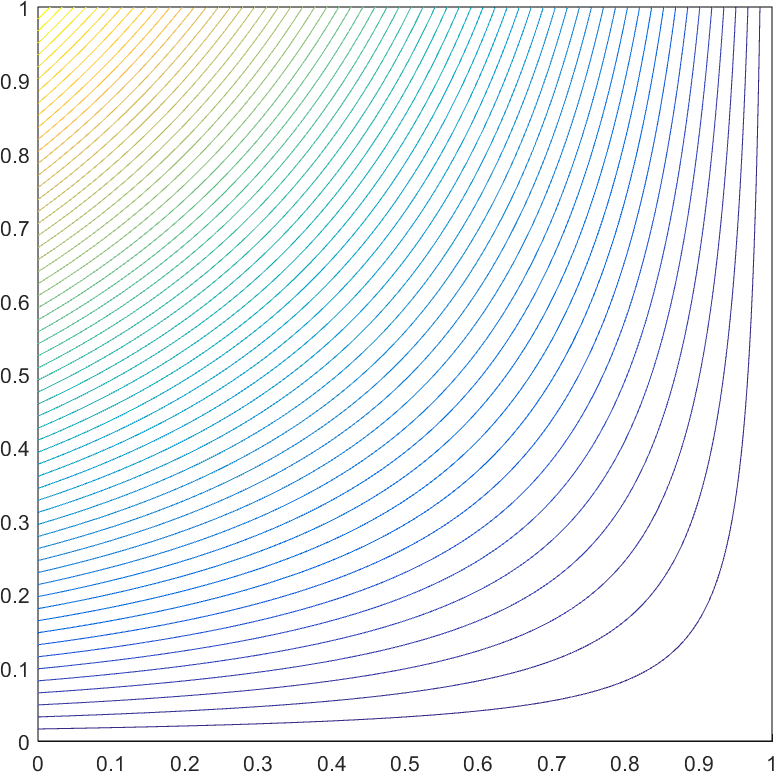
\includegraphics[width=\textwidth]{figures/sec_BF/square_WACHSPRESS1_contour_b4.png}
		\caption{}
	\end{subfigure}
	\hspace{1.5cm}
	\begin{subfigure}[b]{0.39\textwidth}
		\centering
		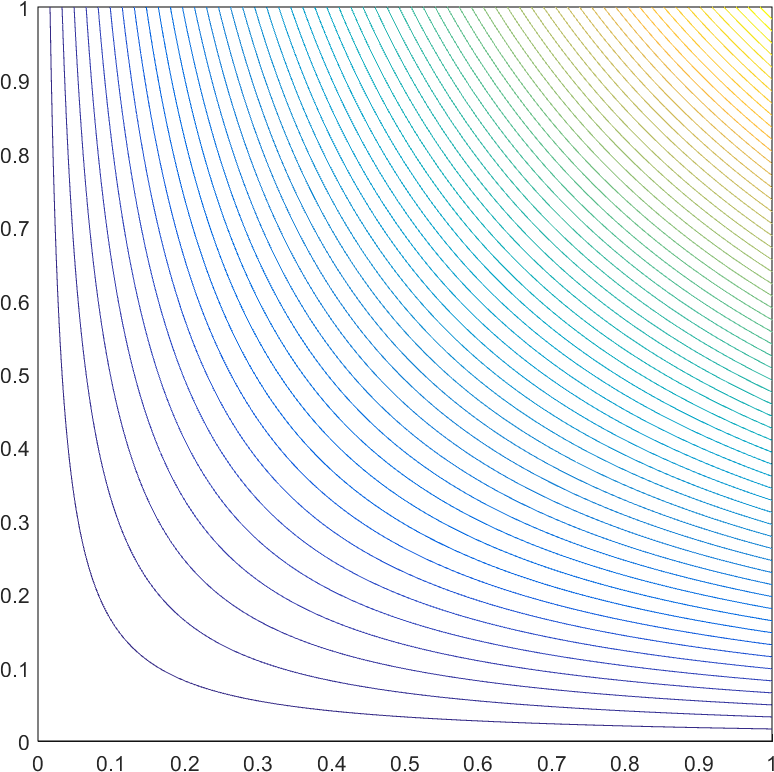
\includegraphics[width=\textwidth]{figures/sec_BF/square_WACHSPRESS1_contour_b3.png}
		\caption{}
	\end{subfigure}
	\vfill
	\begin{subfigure}[b]{0.39\textwidth}
		\centering
		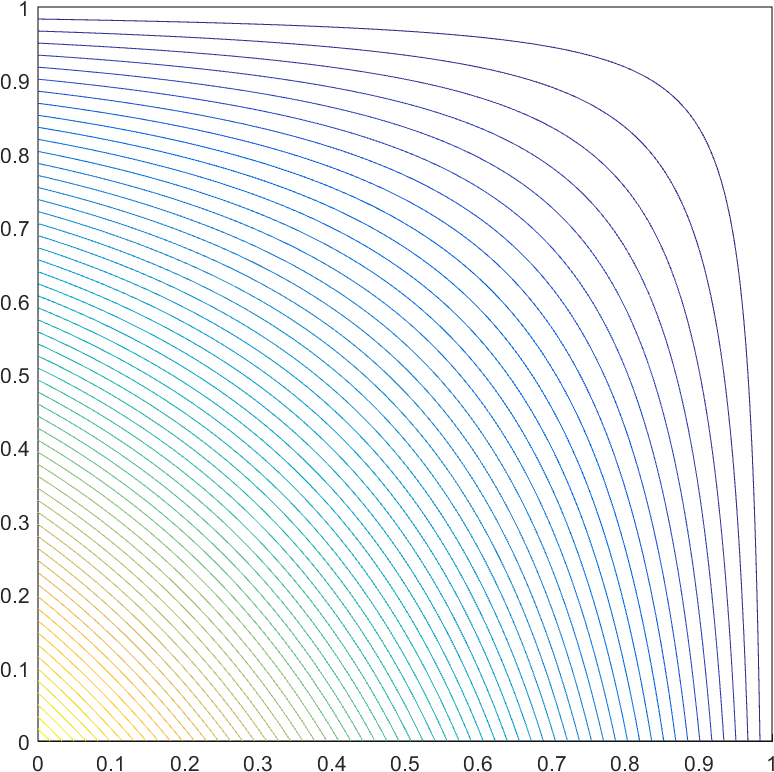
\includegraphics[width=\textwidth]{figures/sec_BF/square_WACHSPRESS1_contour_b1.png}
		\caption{}
	\end{subfigure}
	\hspace{1.5cm}
	\begin{subfigure}[b]{0.39\textwidth}
		\centering
		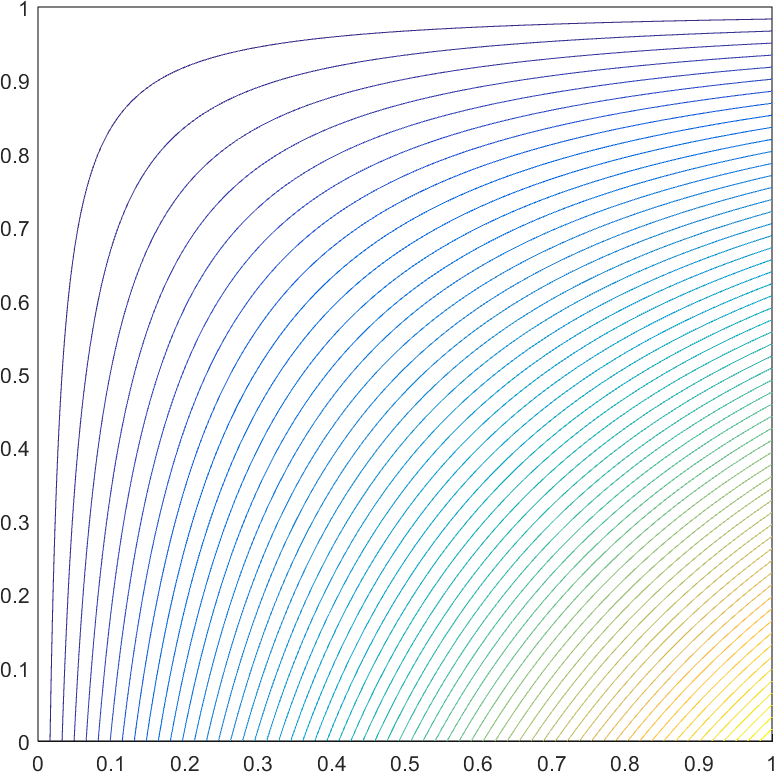
\includegraphics[width=\textwidth]{figures/sec_BF/square_WACHSPRESS1_contour_b2.png}
		\caption{}
	\end{subfigure}
\caption{Contour plots of the linear Wachspress basis functions on the unit square for the vertices located at: (a) (0,1), (b) (1,1), (c) (0,0), and (d) (1,0).}
\label{fig::2D_WACHSPRESS1_unit_square_basis_functions}
\end{figure}

\begin{figure}
\centering
	\begin{subfigure}[b]{0.39\textwidth}
		\centering
		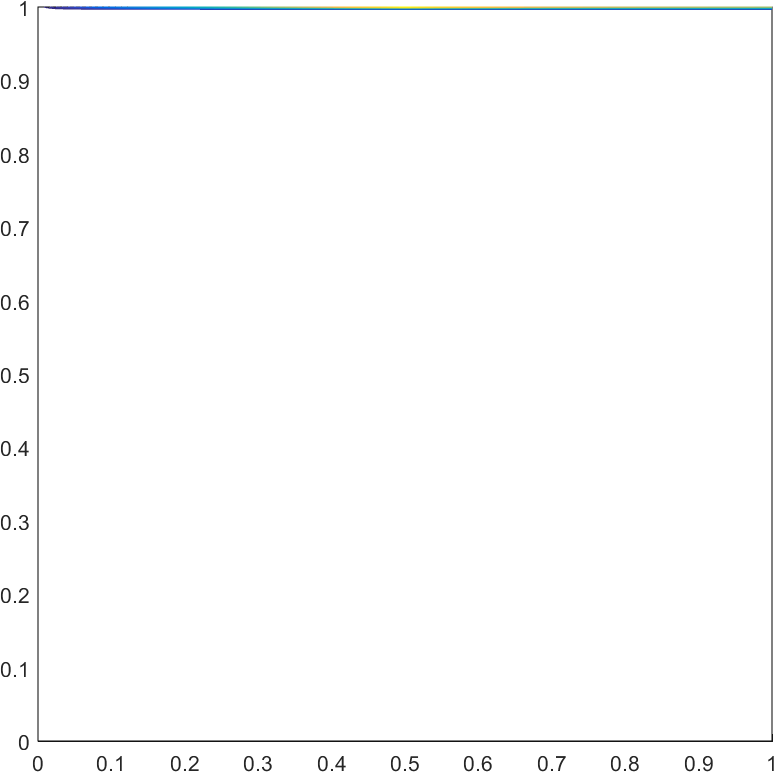
\includegraphics[width=\textwidth]{figures/sec_BF/deg_square_WACHSPRESS1_contour_b4.png}
		\caption{}
	\end{subfigure}
	\vfill
	\begin{subfigure}[b]{0.39\textwidth}
		\centering
		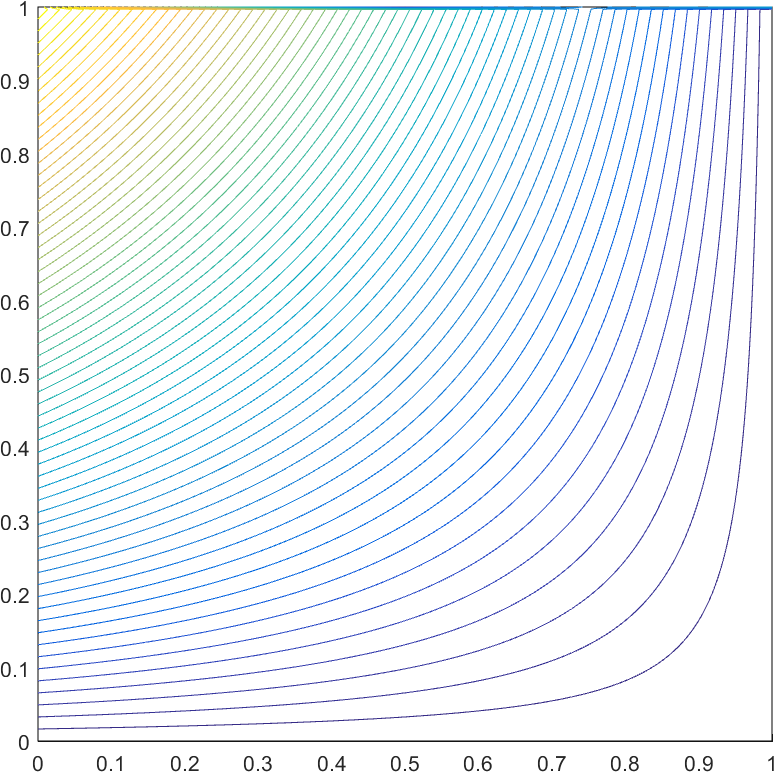
\includegraphics[width=\textwidth]{figures/sec_BF/deg_square_WACHSPRESS1_contour_b5.png}
		\caption{}
	\end{subfigure}
	\hspace{1.5cm}
	\begin{subfigure}[b]{0.39\textwidth}
		\centering
		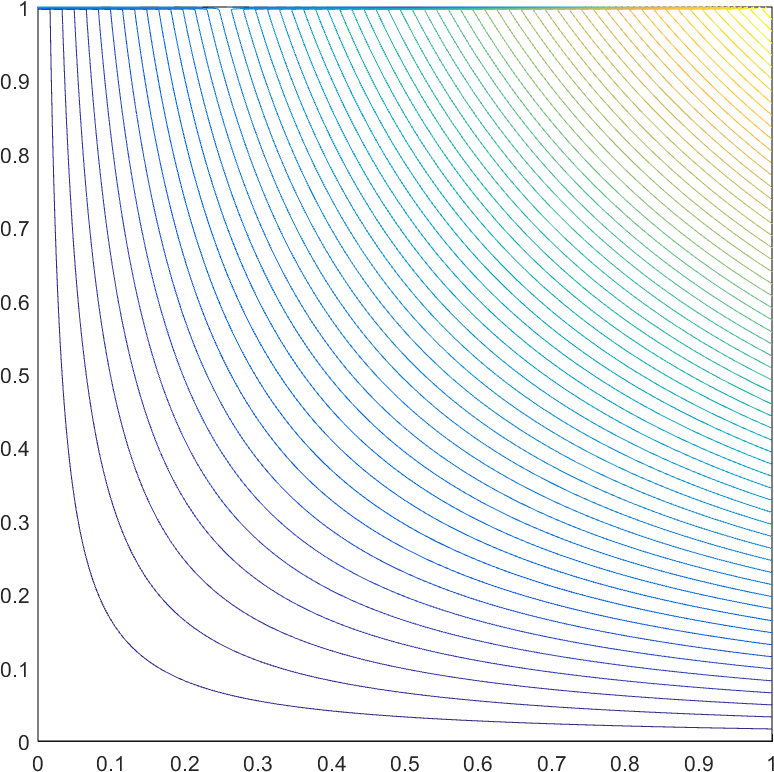
\includegraphics[width=\textwidth]{figures/sec_BF/deg_square_WACHSPRESS1_contour_b3.png}
		\caption{}
	\end{subfigure}
	\vfill
	\begin{subfigure}[b]{0.39\textwidth}
		\centering
		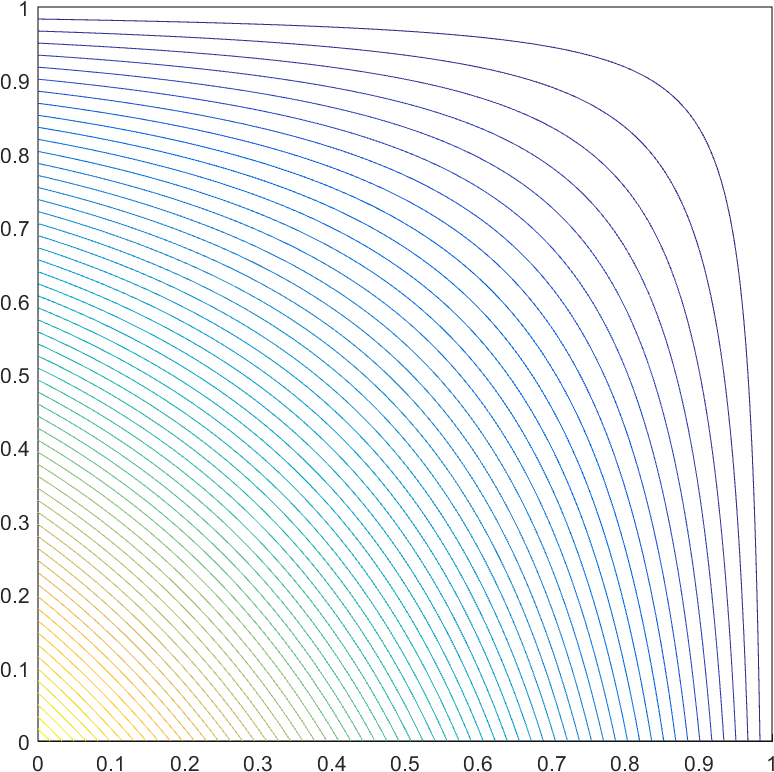
\includegraphics[width=\textwidth]{figures/sec_BF/deg_square_WACHSPRESS1_contour_b1.png}
		\caption{}
	\end{subfigure}
	\hspace{1.5cm}
	\begin{subfigure}[b]{0.39\textwidth}
		\centering
		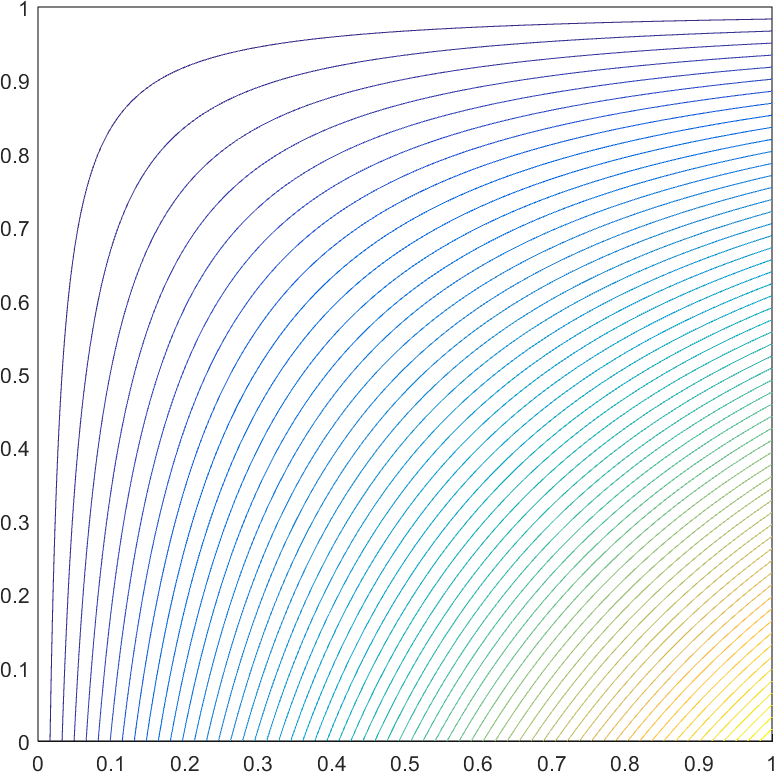
\includegraphics[width=\textwidth]{figures/sec_BF/deg_square_WACHSPRESS1_contour_b2.png}
		\caption{}
	\end{subfigure}
\caption{Contour plots of the linear Wachspress basis functions on the degenerate pentagon for the vertices located at: (a) (1/2,1), (b) (0,1), (c) (1,1), (d) (0,0), and (e) (1,0).}
\label{fig::2D_WACHSPRESS1_deg_square_basis_functions}
\end{figure}

%%%%%%%%%%%%%%%%%%%%%%%%%%%%%%%%%%%%%%%%%%%%%%%%%%%
%%%   SubSection - PWL
\subsection{Piecewise Linear (PWL) Basis Functions}
\label{sec::BF_2DLinear_PWL}

The second linearly-complete 2D polygonal coordinates that we will analyze are the Piecewise Linear (PWL) coordinates proposed by Stone and Adams \cite{ref::PWLD_stone_adams,ref::PWLD_stone_adams_unstructured}. They originally introduced the PWL coordinates to work specifically for the DGFEM transport equation on unstructured quadrilateral and polygonal grids. These coordinates share some similarities with the Wachspress rational functions, but also contain some key differences. The properties of the PWL coordinates that are different from the Wachspress rational functions can be summarized with the following:

\begin{enumerate}
\item PWL works with concave polygons;
\item PWL cannot interpolate on curved surfaces;
\item points on the boundary can be directly evaluated;
\item the PWL integrals can be computed analytically;
\item the PWL functions are only $C^0$ continuous: their gradients are discontinuous within the element.
\end{enumerate}

The 2D PWL functions are defined as combinations of linear triangular functions, with some of them only having measure within a subregion of a polygon. These subregions are formed by triangulating the arbitrary 2D polygon into a set of sub-triangles. Each sub-triangle is defined by two adjacent vertices of the polygon (taken in a counter-clockwise ordering to maintain consistency) and the polygon's centroid, $\vec{r}_{c}$. Looking at Figure \ref{fig::BF_2D_ref_polygon} as an example, sub-triangle $j$ is defined by the points $\{ \vec{x}_j , \vec{x}_{j+1}, \vec{r}_c \}$, which are the polygon's vertices $j$ and $j+1$ and the polygon's centroid. If a polygon $K$ has $N_K$ vertices, then its centroid can be defined by

\begin{equation}
\label{eq::PWL_2D_centroid}
	\vec{r}_{c} =  \sum\displaylimits_{j=1}^{N_K} \alpha_{j}^{K}  \vec{x}_j ,
\end{equation}

\noindent where $\alpha_{j}^{K}$ are the vertex weights functions and, 

\begin{equation}
\label{eq::PWL_2D_vertex_weight_sum}
 \sum\displaylimits_{j=1}^{N_K} \alpha_{j}^{K} = 1.
\end{equation}

\noindent For this work, we continue to use the definition for the vertex weight functions from previous works \cite{ref::PWLD_stone_adams,ref::PWLD_stone_adams_unstructured,bailey2008phd},

\begin{equation}
\label{eq::PWL_2D_vertex_weight_val}
\alpha_{j}^{K} = \frac{1}{N_K} .
\end{equation}

\noindent This means that the vertex weight functions are the same for every vertex and the cell centroid simply becomes the average position of all the vertices. However, we note that care must be taken so that the centroid does not lie on the polygon's boundary. This will cause the PWL functions to no longer have piecewise linearity along the boundary. Using these vertex weight functions, the PWL basis function for vertex $j$, $b_j^{PWL}$, is defined as

\begin{equation}
\label{eq::PWL_2D}
	b_j^{PWL} (x,y) = t_j (x,y) + \alpha_j^K t_c (x,y) .
\end{equation}

\noindent In Eq. (\ref{eq::PWL_2D}), $t_j$ is the standard 2D linear function with unity at vertex $j$ that linearly decreases to zero at the cell center and each adjoining vertex. $t_c$ is the 2D cell ``tent'' function located at $\vec{r}_{c}$ which is unity at the cell center and linearly decreases to zero at each cell vertex. $\alpha_{j}^{K}$ is the weight parameter for vertex $j$ in cell $K$. The functional form of Eq. (\ref{eq::PWL_2D}) with identical vertex weights means that the PWL function for vertex $j$, within the domain of $K$, linearly decreases to a value of $1/N_K$ at the polygonal center. From there, the function linearly decreases to zero on all faces that are not connected to vertex $j$. In Appendix \ref{sec::appendix_BF}, we detail how the 2D PWL coordinates can be analytically integrated using the reference triangle and affine mapping. The gradients of the PWL functions are easy to compute term-by-term in a straightforward manner:

\begin{equation}
\label{eq::PWL_2D_gradients}
	\vec{\nabla} b_j^{PWL} (x,y) = \vec{\nabla} t_j (x,y) + \alpha_j^K \vec{\nabla} t_c (x,y) .
\end{equation}

We now give some example contour plots of the PWL coordinates over different polygons. First, we provide the contour plots for the four PWL functions on the unit square in Figure \ref{fig::2D_PWLD1_unit_square_basis_functions}. In this example it is easy to discern the functional form of Eq. (\ref{eq::PWL_2D}) with the use of constant vertex weights. We clearly see each function linearly decrease from its vertex to the cell center (with a value of $1/N_K$) and then linearly decrease to all non-adjoining faces. Next, Figure \ref{fig::2D_PWLD1_deg_square_basis_functions} provides the contour plots for the PWL functions on a degenerate (weakly-convex) pentagon where a fifth vertex was added to the unit square at ($1/2,1$). Unlike the Wachspress coordinates, the PWL functions work on weakly-convex polygons. The final example we give in Figure \ref{fig::2D_PWLD1_Ldom_basis_functions} is a favorite in the applied mathematics community: the ``L-shaped'' domain. It provides an example of PWL's ability to still be linearly-complete on concave polygons. In this example, the cell centroid was forced to be at the point ($1/3,1/3$) so that it would be inside the polygon.


\begin{figure}
\centering
	\begin{subfigure}[b]{0.39\textwidth}
		\centering
		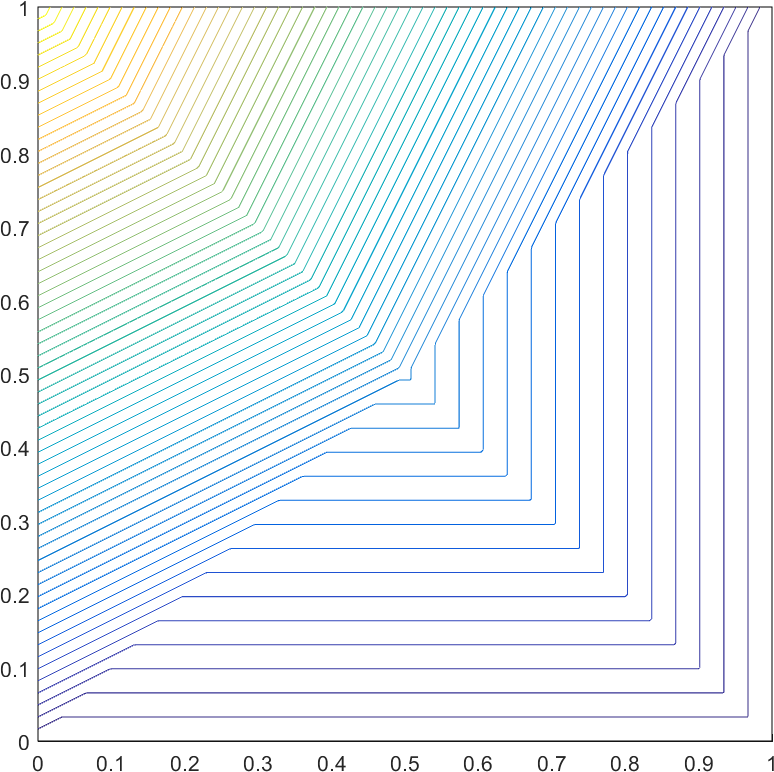
\includegraphics[width=\textwidth]{figures/sec_BF/square_PWLD1_contour_b4.png}
		\caption{}
	\end{subfigure}
	\hspace{1.5cm}
	\begin{subfigure}[b]{0.39\textwidth}
		\centering
		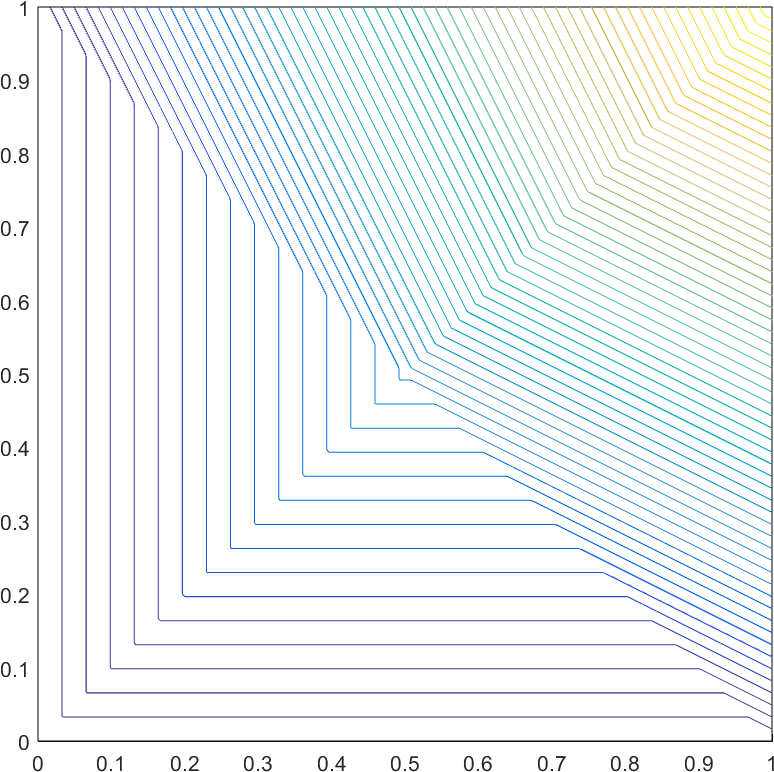
\includegraphics[width=\textwidth]{figures/sec_BF/square_PWLD1_contour_b3.png}
		\caption{}
	\end{subfigure}
	\vfill
	\begin{subfigure}[b]{0.39\textwidth}
		\centering
		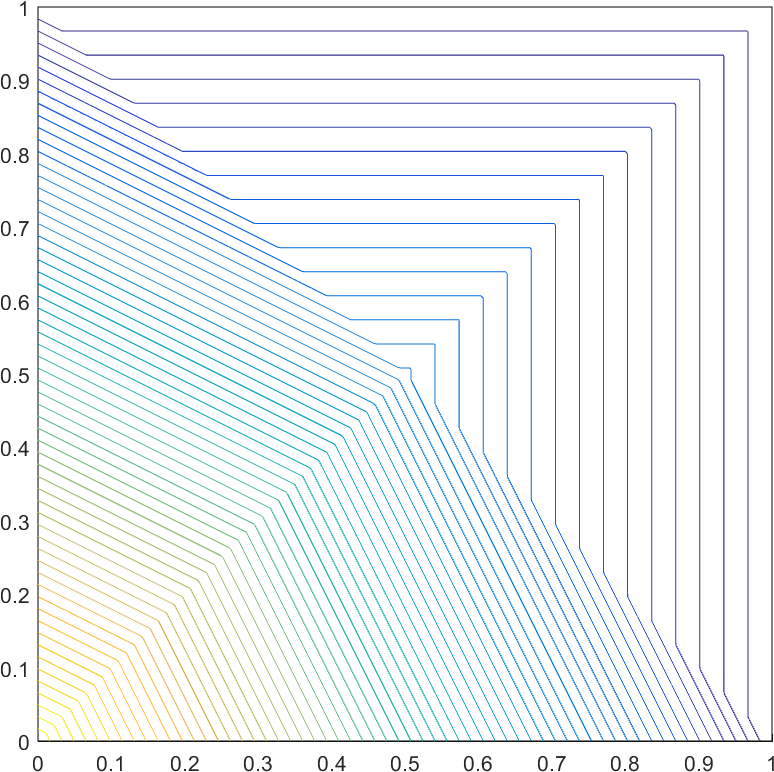
\includegraphics[width=\textwidth]{figures/sec_BF/square_PWLD1_contour_b1.png}
		\caption{}
	\end{subfigure}
	\hspace{1.5cm}
	\begin{subfigure}[b]{0.39\textwidth}
		\centering
		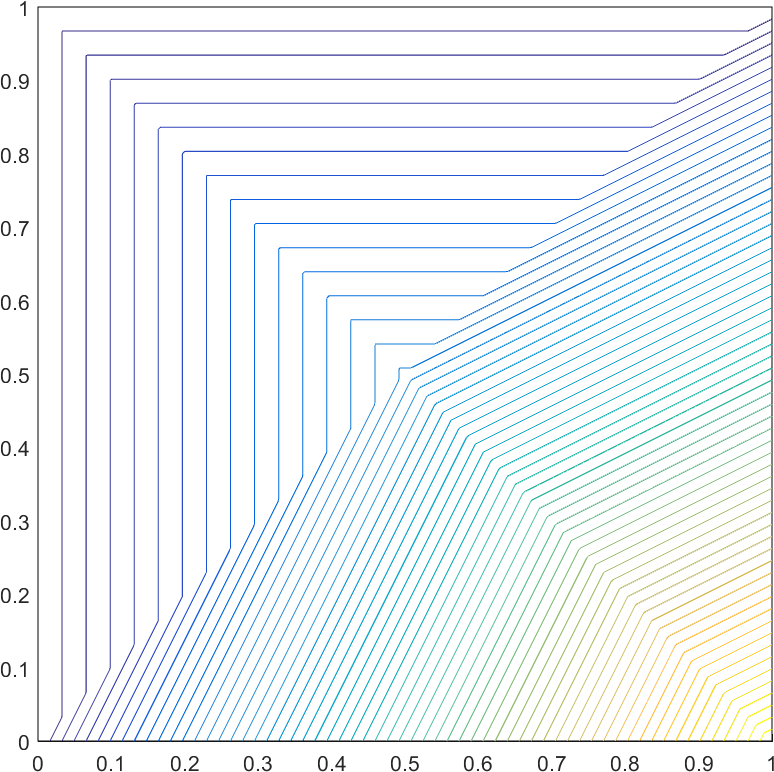
\includegraphics[width=\textwidth]{figures/sec_BF/square_PWLD1_contour_b2.png}
		\caption{}
	\end{subfigure}
\caption{Contour plots of the linear PWL basis functions on the unit square for the vertices located at: (a) (0,1), (b) (1,1), (c) (0,0), and (d) (1,0).}
\label{fig::2D_PWLD1_unit_square_basis_functions}
\end{figure}

\begin{figure}
\centering
	\begin{subfigure}[b]{0.39\textwidth}
		\centering
		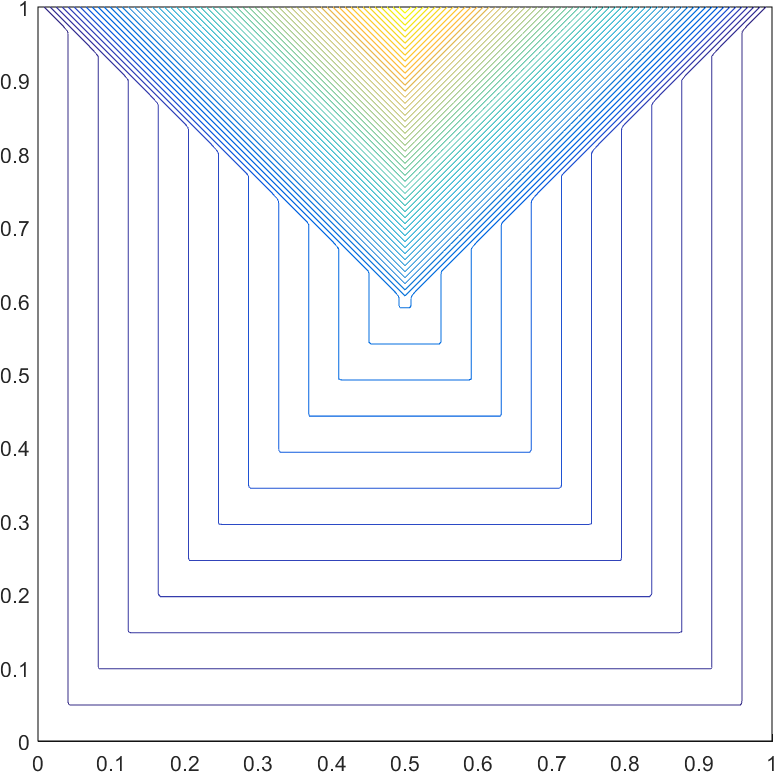
\includegraphics[width=\textwidth]{figures/sec_BF/deg_square_PWLD1_contour_b4.png}
		\caption{}
	\end{subfigure}
	\vfill
	\begin{subfigure}[b]{0.39\textwidth}
		\centering
		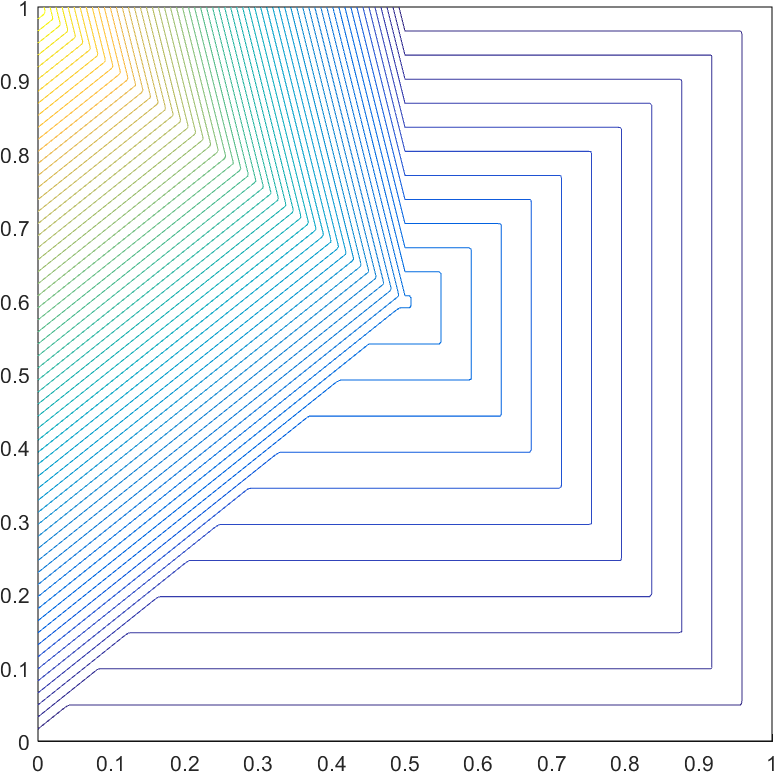
\includegraphics[width=\textwidth]{figures/sec_BF/deg_square_PWLD1_contour_b5.png}
		\caption{}
	\end{subfigure}
	\hspace{1.5cm}
	\begin{subfigure}[b]{0.39\textwidth}
		\centering
		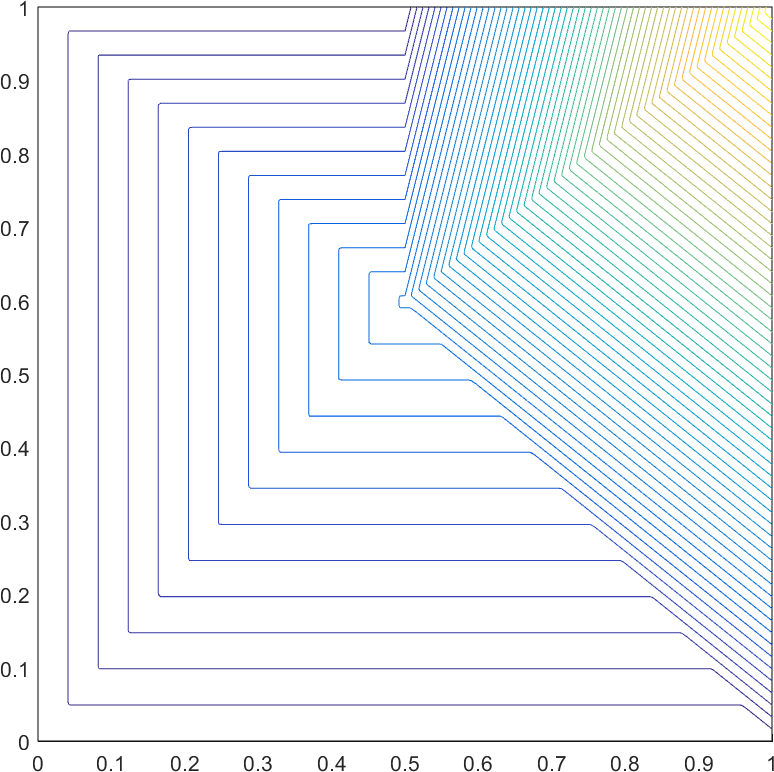
\includegraphics[width=\textwidth]{figures/sec_BF/deg_square_PWLD1_contour_b3.png}
		\caption{}
	\end{subfigure}
	\vfill
	\begin{subfigure}[b]{0.39\textwidth}
		\centering
		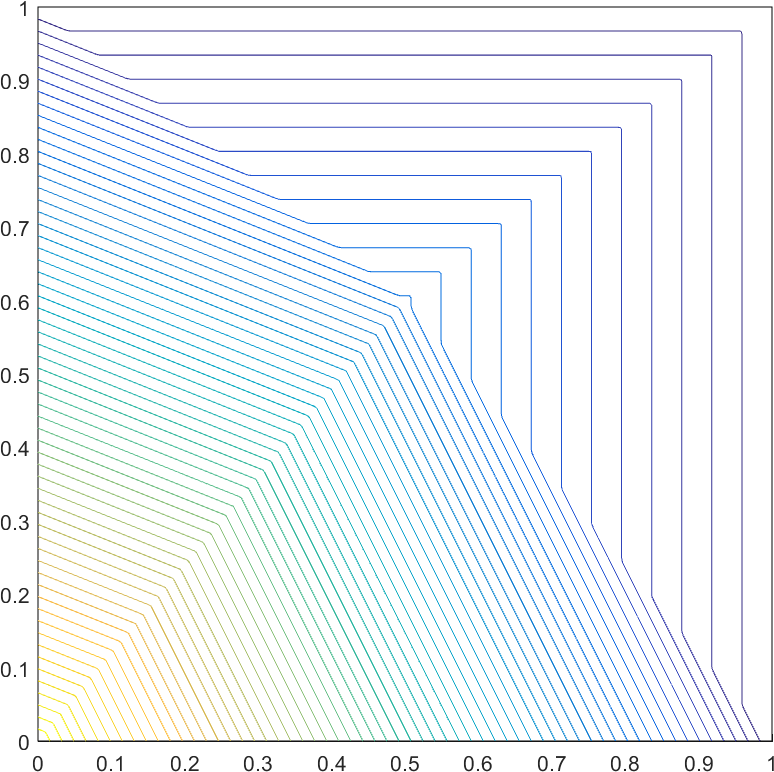
\includegraphics[width=\textwidth]{figures/sec_BF/deg_square_PWLD1_contour_b1.png}
		\caption{}
	\end{subfigure}
	\hspace{1.5cm}
	\begin{subfigure}[b]{0.39\textwidth}
		\centering
		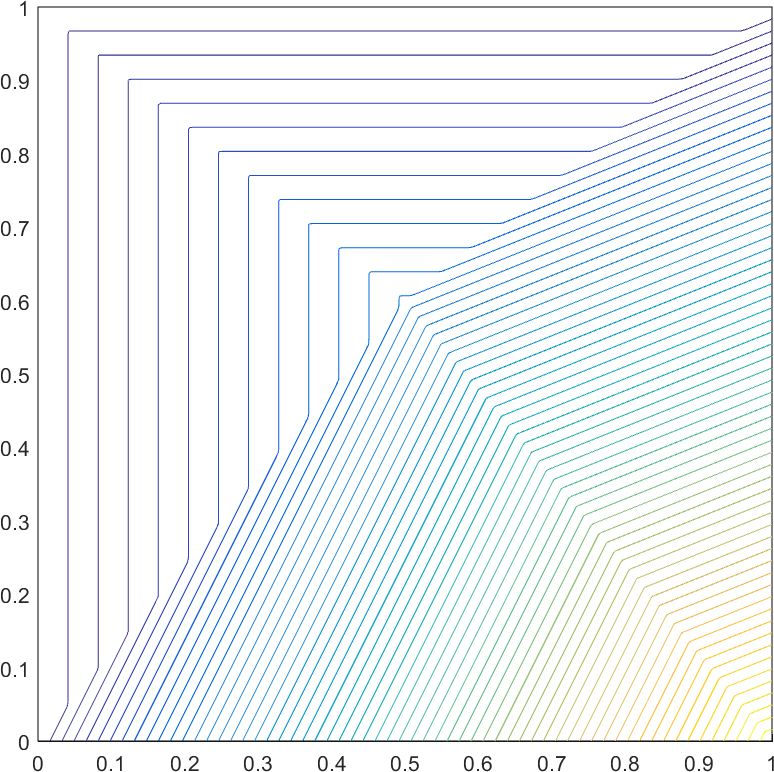
\includegraphics[width=\textwidth]{figures/sec_BF/deg_square_PWLD1_contour_b2.png}
		\caption{}
	\end{subfigure}
\caption{Contour plots of the linear PWL basis functions on the degenerate pentagon for the vertices located at: (a) (1/2,1), (b) (0,1), (c) (1,1), (d) (0,0), and (e) (1,0).}
\label{fig::2D_PWLD1_deg_square_basis_functions}
\end{figure}

\begin{figure}
\centering
	\begin{subfigure}[b]{0.39\textwidth}
		\centering
		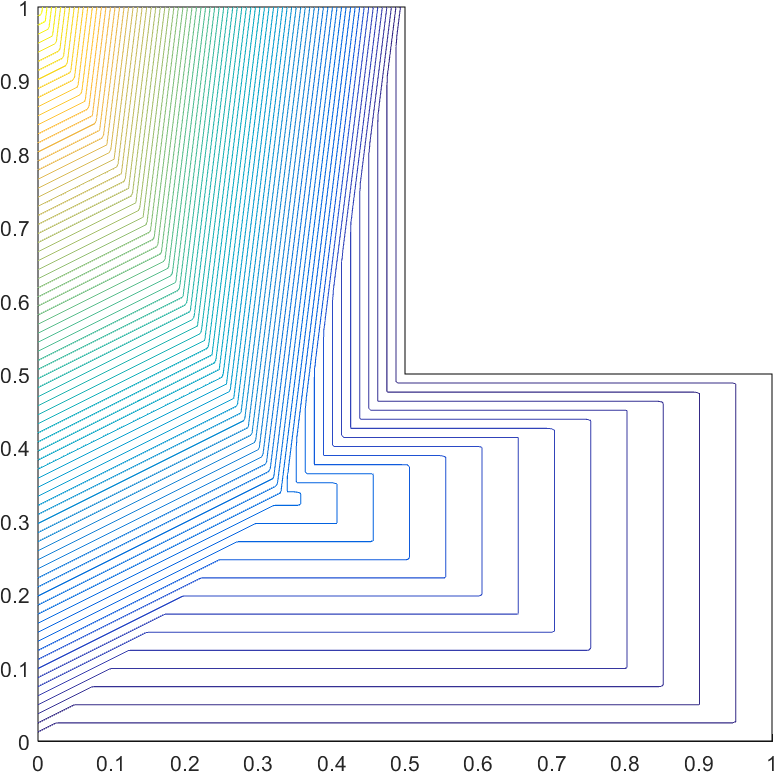
\includegraphics[width=\textwidth]{figures/sec_BF/L-domain_PWLD1_contour_b6.png}
		\caption{}
	\end{subfigure}
	\hspace{1.5cm}
	\begin{subfigure}[b]{0.39\textwidth}
		\centering
		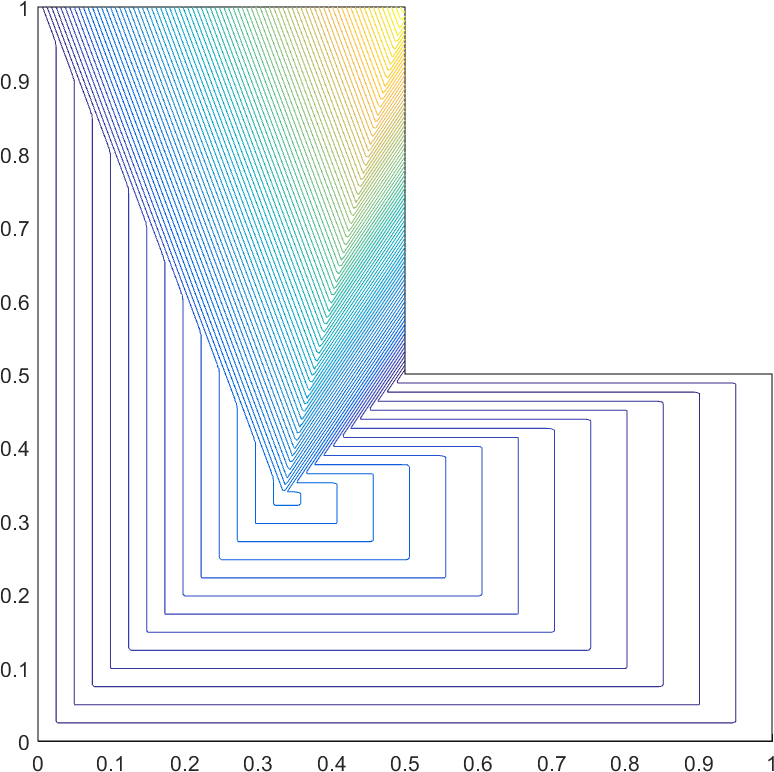
\includegraphics[width=\textwidth]{figures/sec_BF/L-domain_PWLD1_contour_b5.png}
		\caption{}
	\end{subfigure}
	\vfill
	\begin{subfigure}[b]{0.39\textwidth}
		\centering
		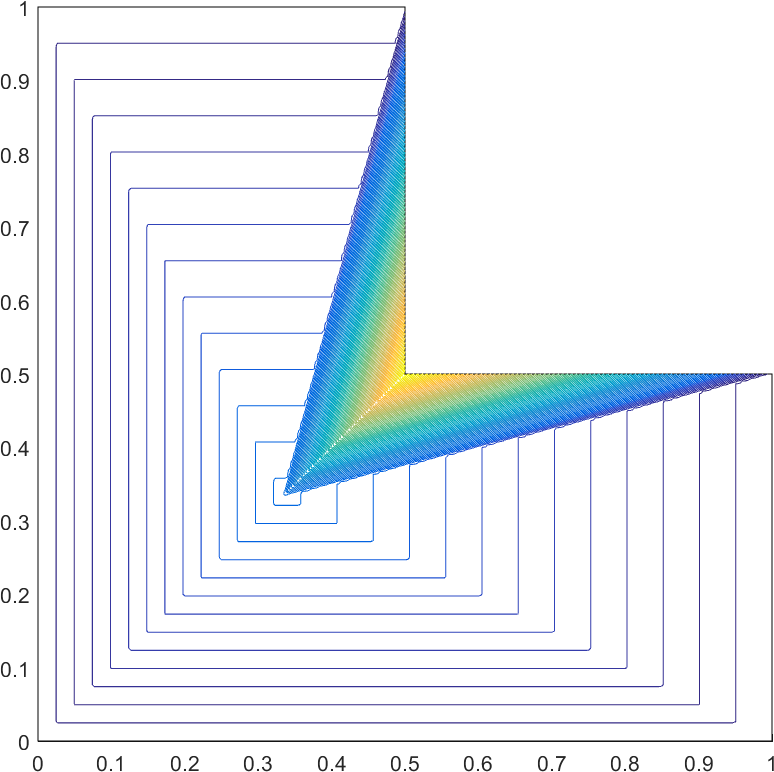
\includegraphics[width=\textwidth]{figures/sec_BF/L-domain_PWLD1_contour_b4.png}
		\caption{}
	\end{subfigure}
	\hspace{1.5cm}
	\begin{subfigure}[b]{0.39\textwidth}
		\centering
		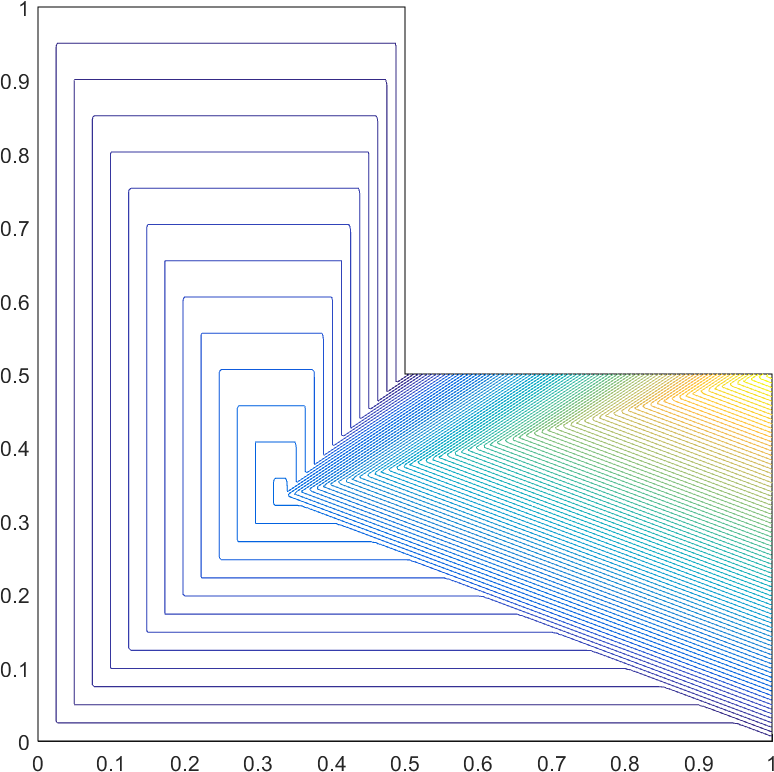
\includegraphics[width=\textwidth]{figures/sec_BF/L-domain_PWLD1_contour_b3.png}
		\caption{}
	\end{subfigure}
	\vfill
	\begin{subfigure}[b]{0.39\textwidth}
		\centering
		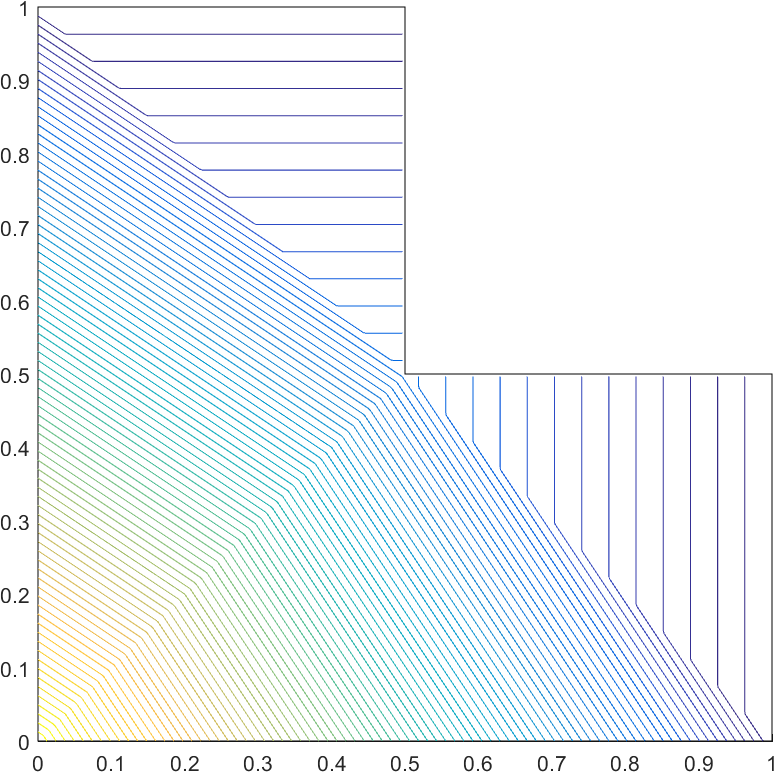
\includegraphics[width=\textwidth]{figures/sec_BF/L-domain_PWLD1_contour_b1.png}
		\caption{}
	\end{subfigure}
	\hspace{1.5cm}
	\begin{subfigure}[b]{0.39\textwidth}
		\centering
		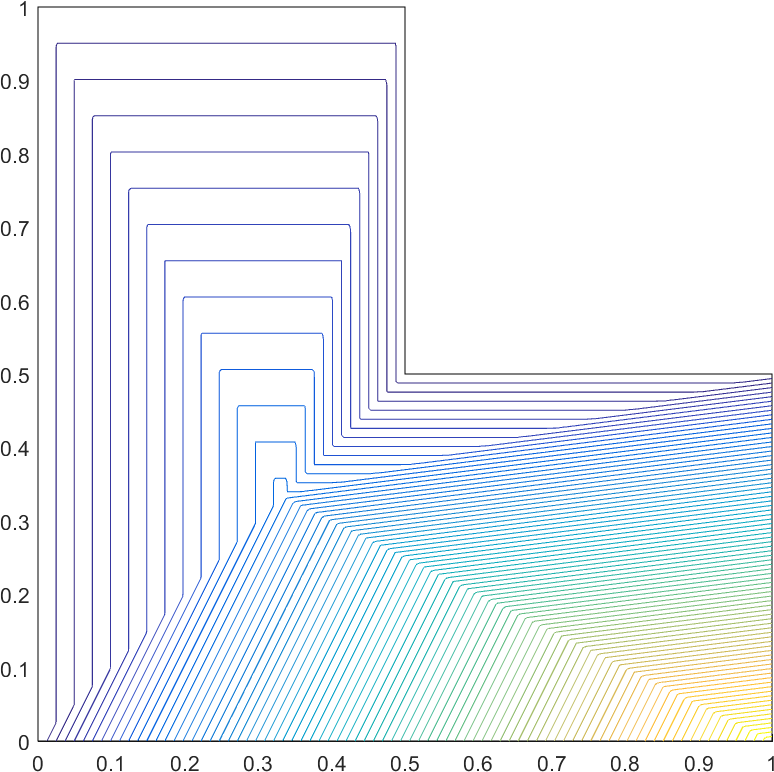
\includegraphics[width=\textwidth]{figures/sec_BF/L-domain_PWLD1_contour_b2.png}
		\caption{}
	\end{subfigure}
\caption{Contour plots of the linear PWL basis functions on the L-shaped domain for the vertices located at: (a) (0,1), (b) (1/2,1), (c) (1/2,1/2), (d) (1,1/2), (e) (0,0), and (f) (1,0).}
\label{fig::2D_PWLD1_Ldom_basis_functions}
\end{figure}





%%%%%%%%%%%%%%%%%%%%%%%%%%%%%%%%%%%%%%%%%%%%%%%%%%%
%%%   SubSection - Mean Value
\subsection{Mean Value Basis Functions}
\label{sec::BF_2DLinear_MV}

At this point, we now introduce the first new polygonal basis set for use with the transport equation: the {\em mean value coordinates} (MV) developed by Floater \cite{floater2003mean}. The original motivation behind the MV coordinates was to approximate harmonic maps on a polygon by a set of piecewise linear maps over a triangulation of the polygon for use in computer aided graphic design. Injectivity is preserved if the interpolatory function is {\em harmonic} over the piecewise linear maps. This can be shown by expressing a $C^2$ function $u$ over each sub-triangle, $\mathcal{T}$, of the triangulated polygon and have it satisfy the Laplace equation,

\begin{equation}
\label{eq::BF_MV_laplace}
\nabla^2 u = 0 ,
\end{equation}

\noindent where $u(\vec{r}_b) = u_0$ consists of a piecewise linear Dirichlet boundary condition ($\vec{r}_b \in \partial \mathcal{T}$) for each triangulation. Then, by use of the mean value theorem (where this coordinate system got its name), the mean value function at vertex $j$, $b_{j}^{MV}$, for a polygon $K$ with $N_K$ vertices can be given by

\begin{equation}
\label{eq::BF_MV_BF}
b_{j}^{MV} (\vec{x}) = \frac{w_j (\vec{x}) }{\sum\limits_{i=1}^{N_K} w_i (\vec{x})} ,
\end{equation}

\noindent where the mean value weight function for vertex $j$, $w_j$, has the following definition:

\begin{equation}
\label{eq::BF_MV_weights}
w_j (\vec{x})  = \frac{\tan(\alpha_{j-1} / 2) + \tan(\alpha_j / 2)}{|\vec{x}_j - \vec{x}|}.
\end{equation}

\noindent This weight simply consists of the addition of the two tangent functions (where the angles are given in Figure \ref{fig::BF_2D_ref_polygon}) that is then divided through by the distance between the vertex $j$ and the point of interest, $\vec{x}$. Through careful observation of Eq. (\ref{eq::BF_MV_weights}), we can see that these MV weights are undefined on certain portions of the polygon's boundary, $\partial K$, in a similar way to the Wachspress coordinates. However, the limits of the coordinates are bounded on the polygon's faces and vertices, and we rigorously show this in Appendix \ref{sec::appendix_BF}.

We now give the form of the mean value gradients. Since the mean value coordinates given by Eq. (\ref{eq::BF_MV_BF}) have the same form as the Wachspress coordinates, their gradients can be expressed in an identical manner. The gradients of the mean value coordinates can be expressed as

\begin{equation}
\label{eq::BF_mv_gradient}
\vec{\nabla} b_{j}^{MV}(\vec{x}) = b_{j}^{MV} (\vec{x}) \left( \vec{R}_j  (\vec{x})- \sum\displaylimits_{i}   b_{i}^{MV} (\vec{x}) \vec{R}_i (\vec{x}) \right) ,
\end{equation}

\noindent where the reduced gradient, $\vec{R}_j $, still has the same definition from Eq. (\ref{eq::BF_wach_reduced_grad}). If we define $t_j=\tan(\alpha_j/2)$ and $t_{j-1}=\tan(\alpha_{j-1}/2)$, then after extensive algebra, the mean value reduced gradients are

\begin{equation}
\label{eq::BF_mv_red_grad_form}
\vec{R}_j  = \left( \frac{t_{j-1}}{t_{j-1} + t_{j}} \right) \frac{\{  \vec{c}_{j-1} \}}{\sin (  \alpha_{j-1} )} +  \left( \frac{t_{j}}{t_{j-1} + t_{j}} \right) \frac{\{  \vec{c}_{j} \}}{\sin (  \alpha_{j} )}+ \frac{\vec{g}_j}{|\vec{x}_i - \vec{x}|},
\end{equation}

\noindent where

\begin{equation}
\label{eq::BF_mv_red_cval}
\vec{c}_j = \frac{\vec{g}_{j}}{|\vec{x}_j - \vec{x}|} - \frac{\vec{g}_{j+1}}{|\vec{x}_{j+1} - \vec{x}|},
\end{equation}

\noindent and

\begin{equation}
\label{eq::BF_mv_red_gval}
\vec{g}_j = \frac{\vec{x}_j - \vec{x}}{|\vec{x}_j - \vec{x}|},
\end{equation}

\noindent and 

\begin{equation}
\label{eq::BF_mv_red_flop}
\{  \vec{u} \} = \left( - u_2 , u_1  \right). 
\end{equation}

\noindent While this direct form for the MV coordinates is more complicated than the last two coordinates presented, it is still easily programmable. The interested reader can look in the appendix of \cite{floater2015generalized} for MATLAB code to compute these gradients.

We again provide example contour plots of the MV coordinates, and we use the same polygonal shapes that we showed for the PWL coordinates. Figure \ref{fig::2D_MV1_unit_square_basis_functions} gives the MV coordinates on the unit square. Like the Wachspress functions, the MV coordinates are smoothly varying within the domain of the polygon and possess continuous derivatives. Next in Figure \ref{fig::2D_MV1_deg_square_basis_functions}, we give the example contour plots for the degenerate pentagon which is formed by inserting a vertex into the unit square at $(1/2,1)$. Finally, Figure \ref{fig::2D_MV1_Ldom_basis_functions} gives the contour plots for the linear mean value coordinates on the L-shaped domain. We see that the linear mean value coordinates are applicable to interpolation on concave polygons.

\begin{figure}
\centering
	\begin{subfigure}[b]{0.39\textwidth}
		\centering
		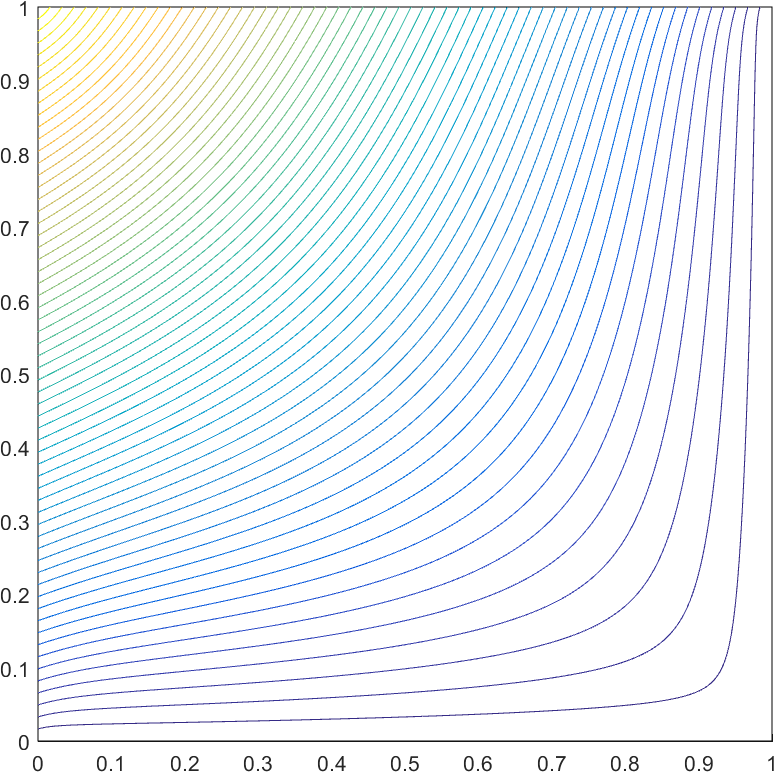
\includegraphics[width=\textwidth]{figures/sec_BF/square_MV1_contour_b4.png}
		\caption{}
	\end{subfigure}
	\hspace{1.5cm}
	\begin{subfigure}[b]{0.39\textwidth}
		\centering
		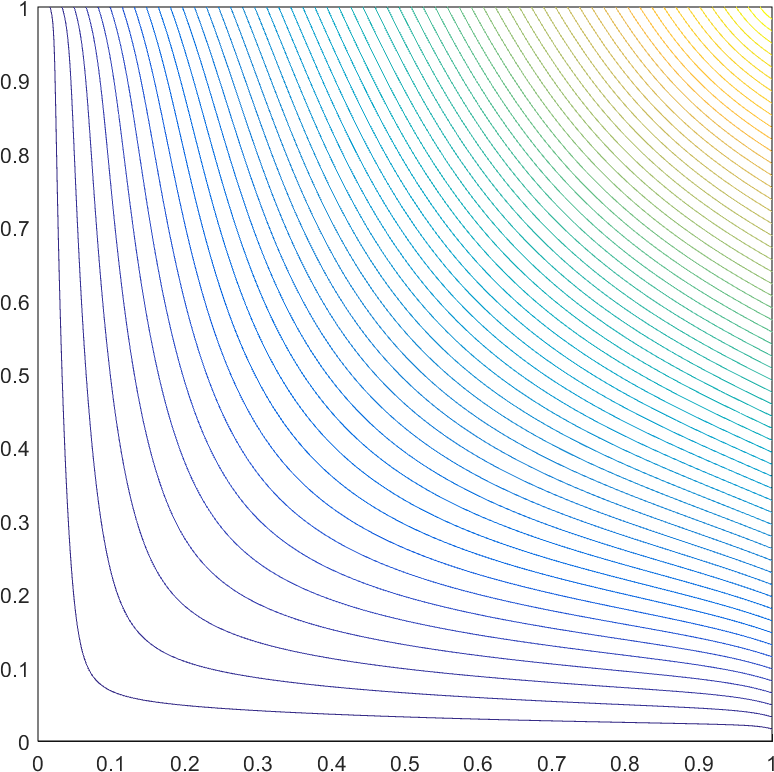
\includegraphics[width=\textwidth]{figures/sec_BF/square_MV1_contour_b3.png}
		\caption{}
	\end{subfigure}
	\vfill
	\begin{subfigure}[b]{0.39\textwidth}
		\centering
		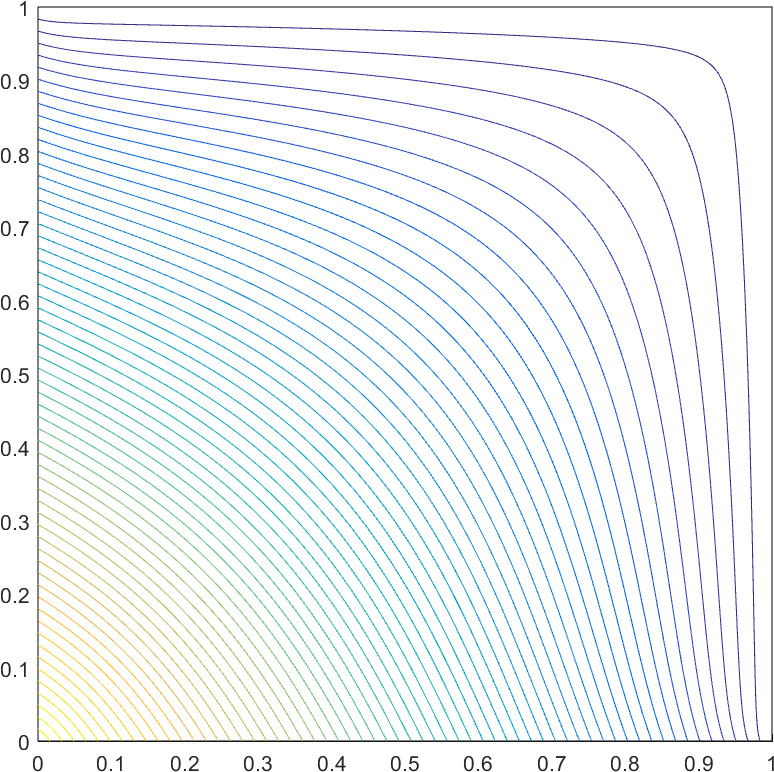
\includegraphics[width=\textwidth]{figures/sec_BF/square_MV1_contour_b1.png}
		\caption{}
	\end{subfigure}
	\hspace{1.5cm}
	\begin{subfigure}[b]{0.39\textwidth}
		\centering
		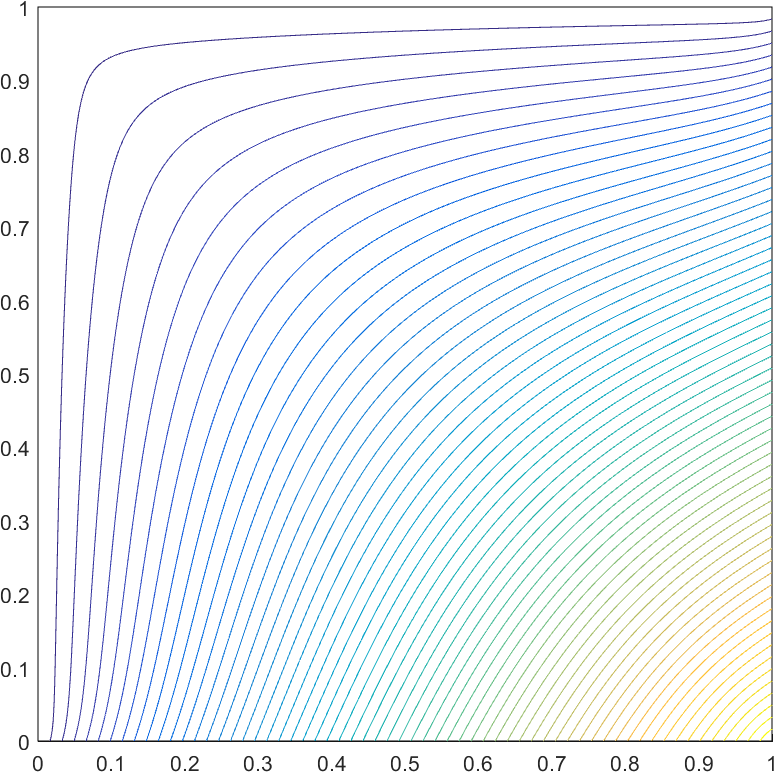
\includegraphics[width=\textwidth]{figures/sec_BF/square_MV1_contour_b2.png}
		\caption{}
	\end{subfigure}
\caption{Contour plots of the linear mean value basis functions on the unit square for the vertices located at: (a) (0,1), (b) (1,1), (c) (0,0), and (d) (1,0).}
\label{fig::2D_MV1_unit_square_basis_functions}
\end{figure}

\begin{figure}
\centering
	\begin{subfigure}[b]{0.39\textwidth}
		\centering
		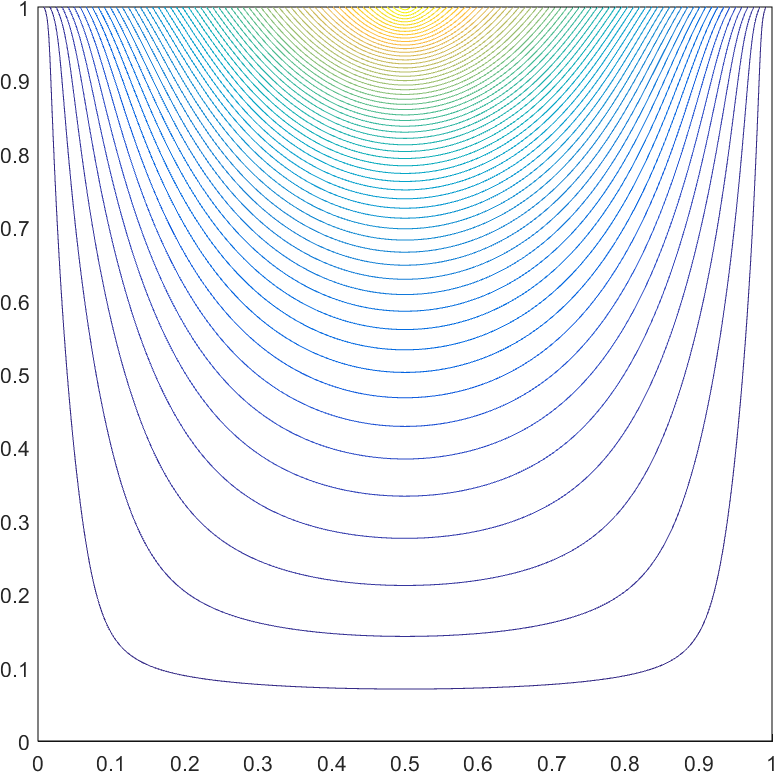
\includegraphics[width=\textwidth]{figures/sec_BF/deg_square_MV1_contour_b4.png}
		\caption{}
	\end{subfigure}
	\vfill
	\begin{subfigure}[b]{0.39\textwidth}
		\centering
		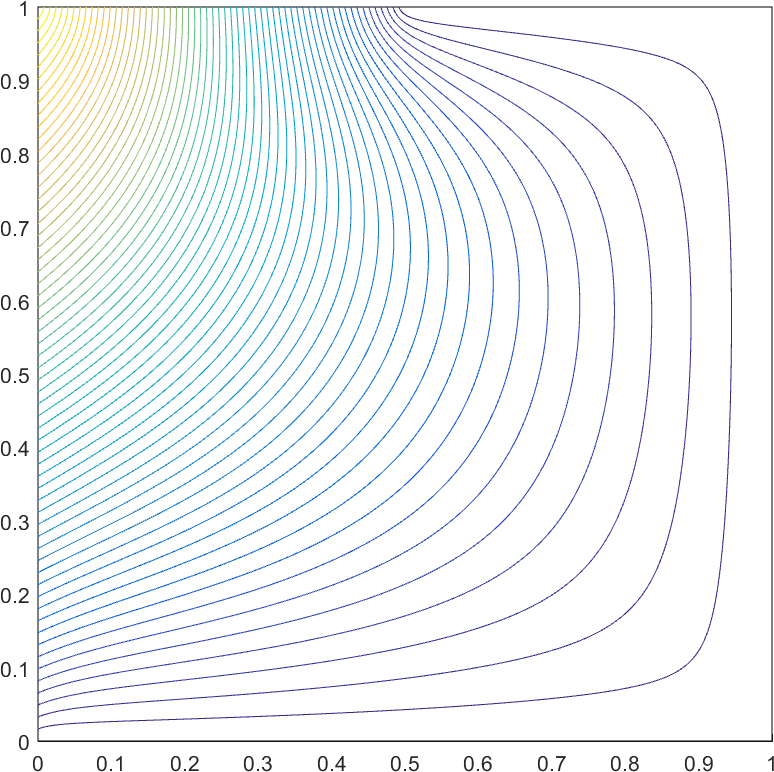
\includegraphics[width=\textwidth]{figures/sec_BF/deg_square_MV1_contour_b5.png}
		\caption{}
	\end{subfigure}
	\hspace{1.5cm}
	\begin{subfigure}[b]{0.39\textwidth}
		\centering
		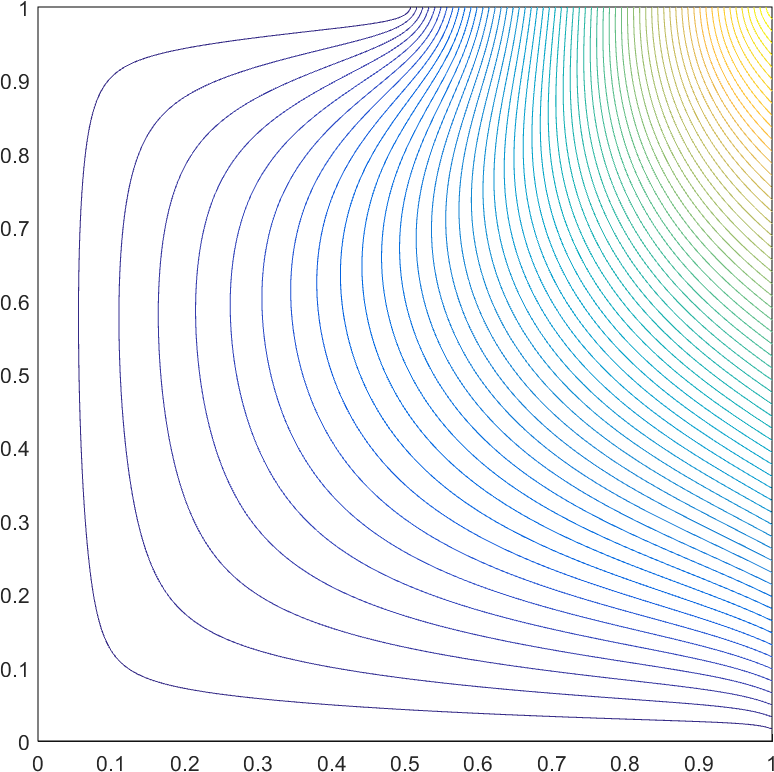
\includegraphics[width=\textwidth]{figures/sec_BF/deg_square_MV1_contour_b3.png}
		\caption{}
	\end{subfigure}
	\vfill
	\begin{subfigure}[b]{0.39\textwidth}
		\centering
		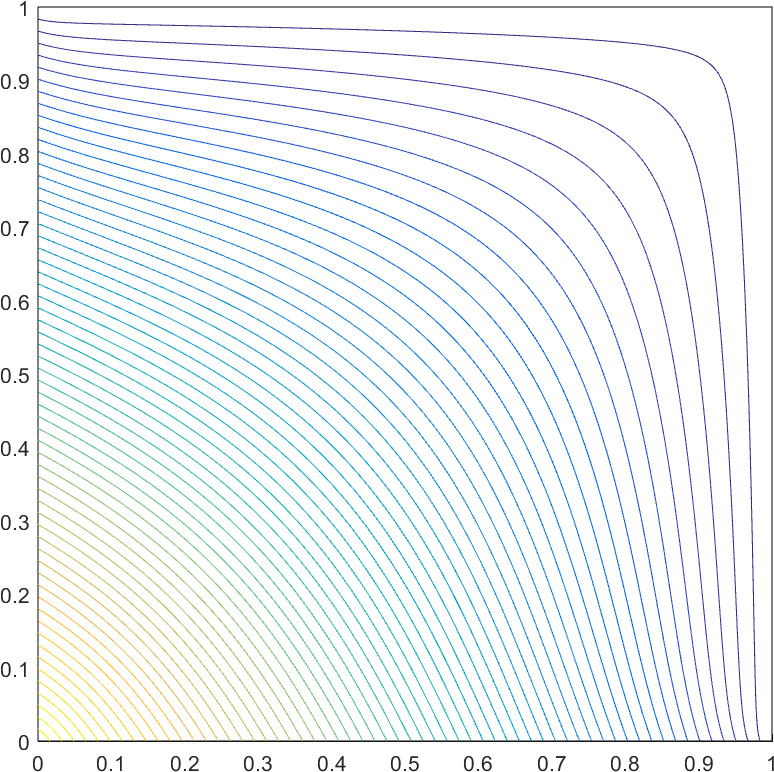
\includegraphics[width=\textwidth]{figures/sec_BF/deg_square_MV1_contour_b1.png}
		\caption{}
	\end{subfigure}
	\hspace{1.5cm}
	\begin{subfigure}[b]{0.39\textwidth}
		\centering
		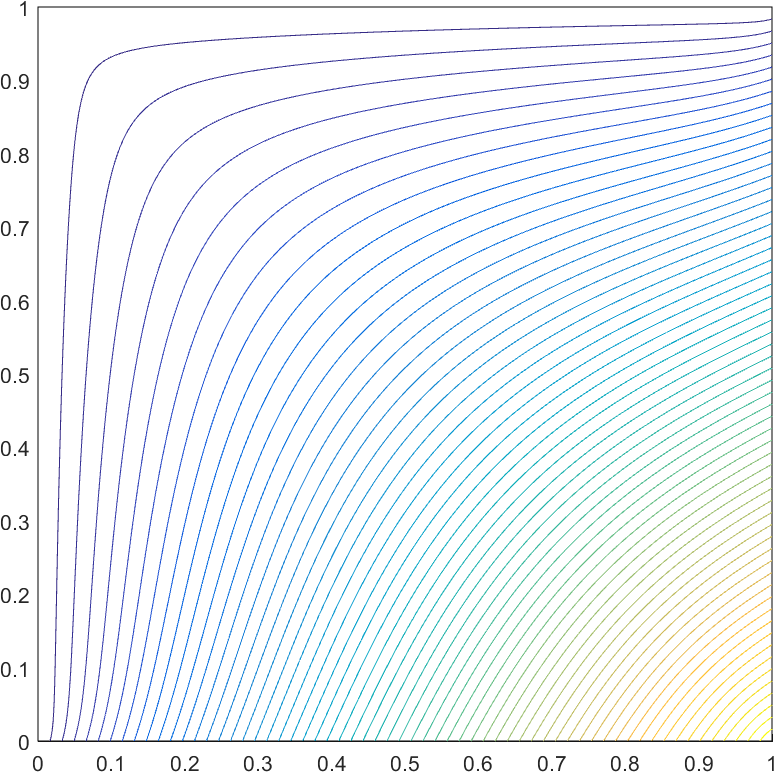
\includegraphics[width=\textwidth]{figures/sec_BF/deg_square_MV1_contour_b2.png}
		\caption{}
	\end{subfigure}
\caption{Contour plots of the linear mean value basis functions on the degenerate pentagon for the vertices located at: (a) (1/2,1), (b) (0,1), (c) (1,1), (d) (0,0), and (e) (1,0).}
\label{fig::2D_MV1_deg_square_basis_functions}
\end{figure}

\begin{figure}
\centering
	\begin{subfigure}[b]{0.39\textwidth}
		\centering
		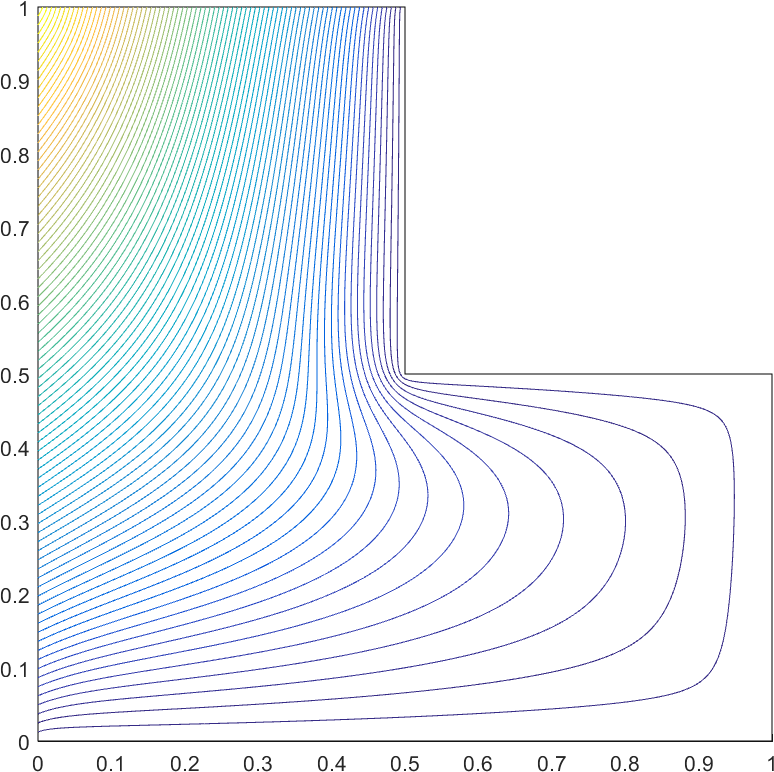
\includegraphics[width=\textwidth]{figures/sec_BF/L-domain_MV1_contour_b6.png}
		\caption{}
	\end{subfigure}
	\hspace{1.5cm}
	\begin{subfigure}[b]{0.39\textwidth}
		\centering
		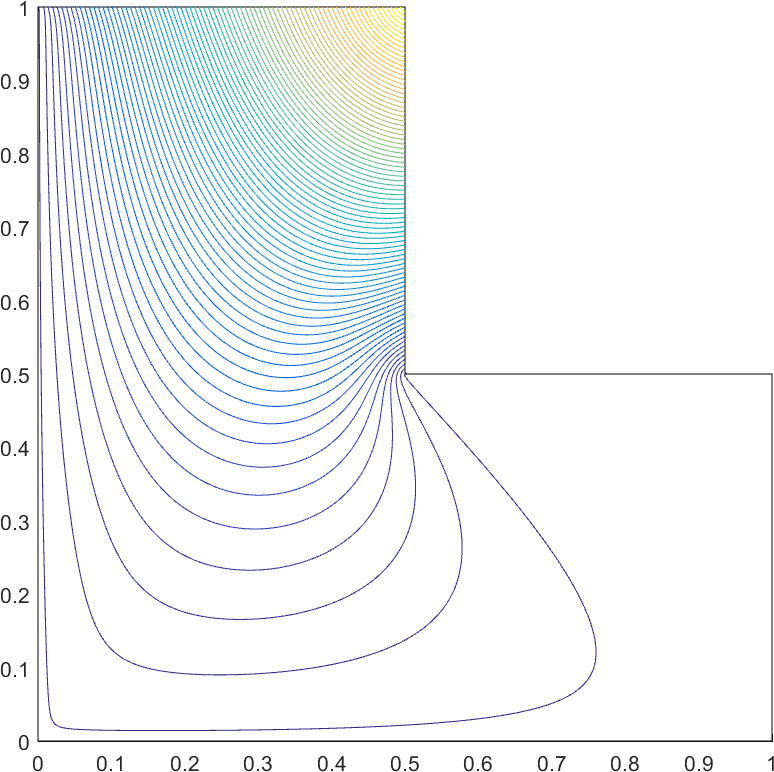
\includegraphics[width=\textwidth]{figures/sec_BF/L-domain_MV1_contour_b5.png}
		\caption{}
	\end{subfigure}
	\vfill
	\begin{subfigure}[b]{0.39\textwidth}
		\centering
		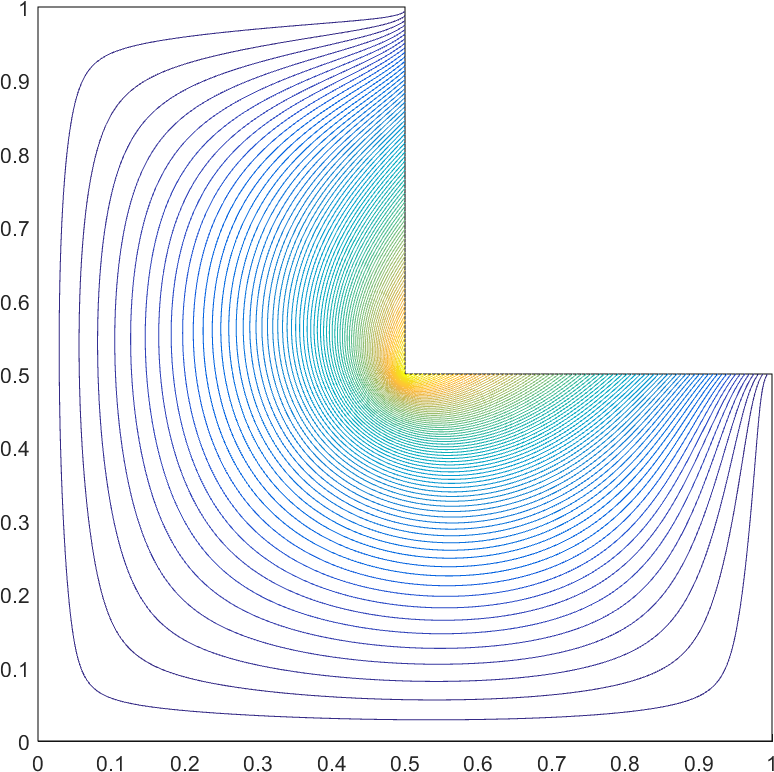
\includegraphics[width=\textwidth]{figures/sec_BF/L-domain_MV1_contour_b4.png}
		\caption{}
	\end{subfigure}
	\hspace{1.5cm}
	\begin{subfigure}[b]{0.39\textwidth}
		\centering
		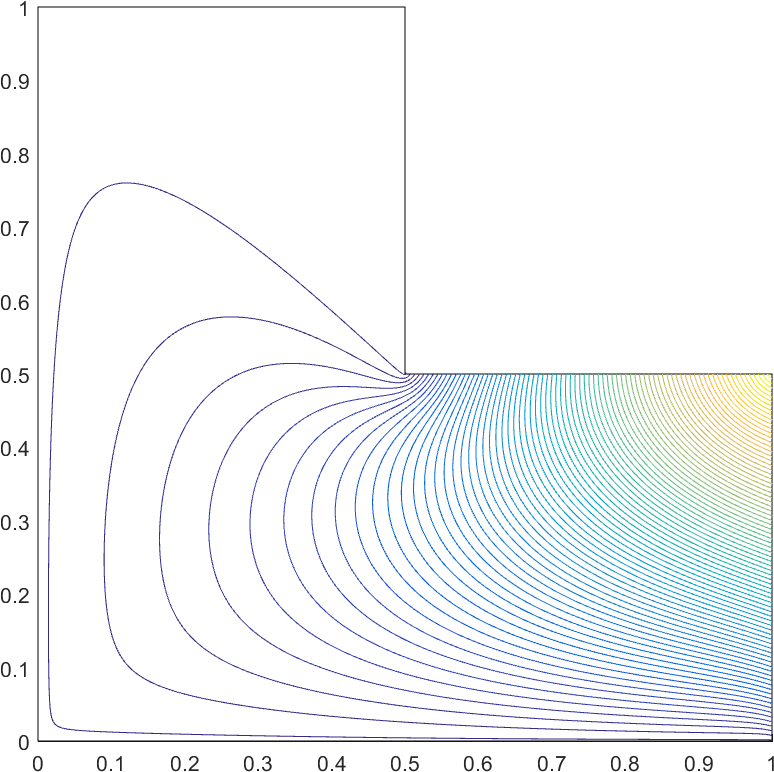
\includegraphics[width=\textwidth]{figures/sec_BF/L-domain_MV1_contour_b3.png}
		\caption{}
	\end{subfigure}
	\vfill
	\begin{subfigure}[b]{0.39\textwidth}
		\centering
		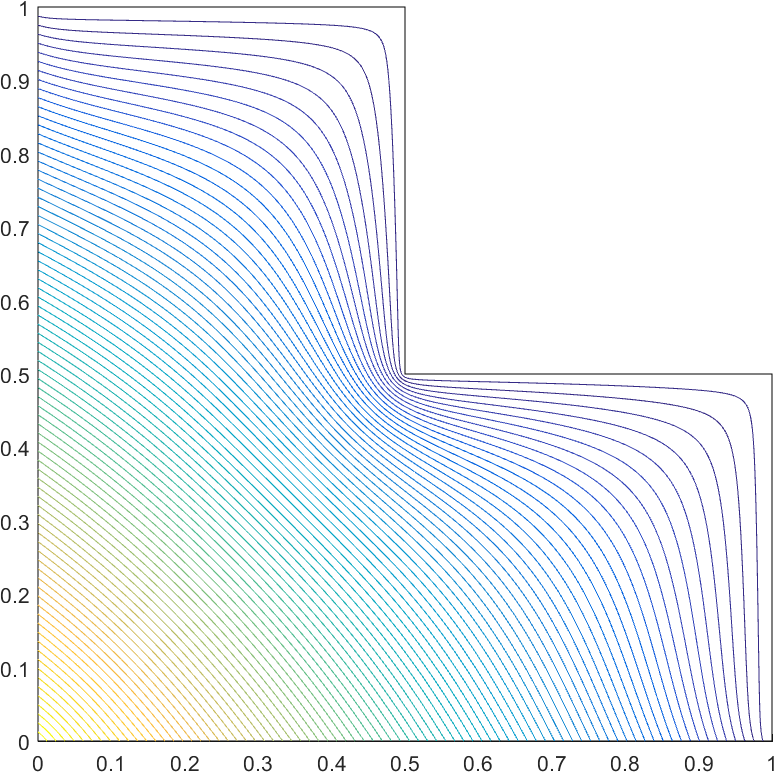
\includegraphics[width=\textwidth]{figures/sec_BF/L-domain_MV1_contour_b1.png}
		\caption{}
	\end{subfigure}
	\hspace{1.5cm}
	\begin{subfigure}[b]{0.39\textwidth}
		\centering
		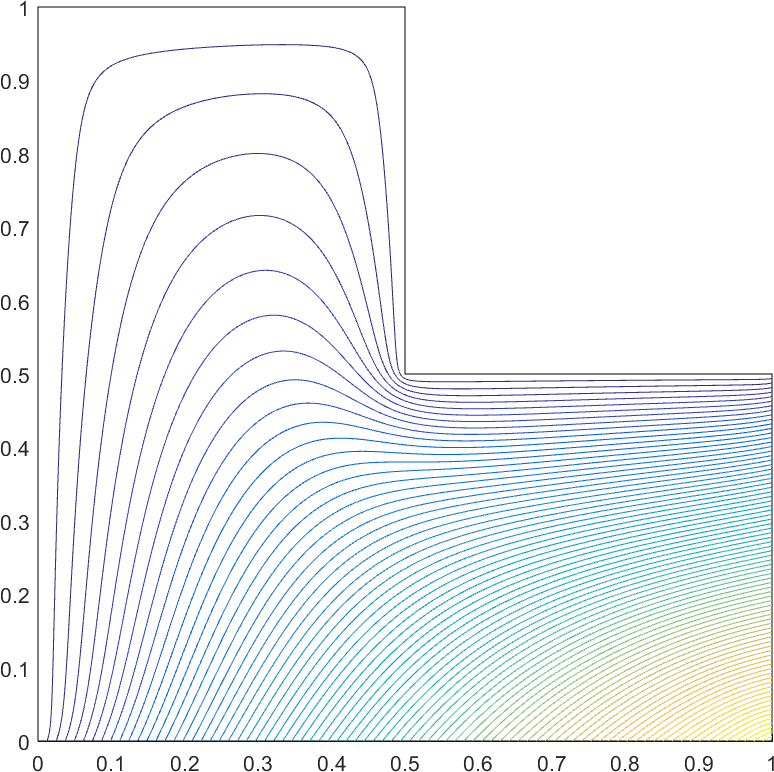
\includegraphics[width=\textwidth]{figures/sec_BF/L-domain_MV1_contour_b2.png}
		\caption{}
	\end{subfigure}
\caption{Contour plots of the linear mean value basis functions on the L-shaped domain for the vertices located at: (a) (0,1), (b) (1/2,1), (c) (1/2,1/2), (d) (1,1/2), (e) (0,0), and (f) (1,0).}
\label{fig::2D_MV1_Ldom_basis_functions}
\end{figure}





%%%%%%%%%%%%%%%%%%%%%%%%%%%%%%%%%%%%%%%%%%%%%%%%%%%
%%%   SubSection - Maximum Entropy
\subsection{Maximum Entropy Basis Functions}
\label{sec::BF_2DLinear_ME}

The final linearly-complete 2D basis functions that we will analyze in this work are generated by use of the {\em maximum entropy coordinates} (ME) \cite{sukumar2004construction,arroyo2006local,hormann2008maximum}. These coordinates have garnered much interest in different fields because their functional forms can be tailored based on the application. The principle of maximum entropy stems from the concept of {\em Shannon entropy} \cite{shannon1948mathematical}. If we define a functional for the Shannon entropy as $H$, then its maximum will lead to the least-biased statistical inference for some set of testable constraints \cite{jaynes1957information}. For the application of FEM analysis, these testable constraints correspond to those given in Eq. (\ref{eq::BF_linear_interp_req_vector}). For $N_K$ discrete probability functions (corresponding to the $N_K$ vertex functions on polygon $K$), the functional form for the Shannon entropy can be given by

\begin{equation}
\label{eq::BF_ME_H}
H(b, m) = - \sum\displaylimits_{j=1}^{N_K} b_j \log \left(  \frac{b_j}{m_j} \right) , 
\end{equation}

\noindent where $m_j$ is called the prior distribution. These prior distributions are a key component of Bayesian inference \cite{kullback1951information,jaynes1963information}. If ($b_j^{ME} (\vec{x})  ,j=1,...,N_K$) is the solution of the following constrained optimization problem

\begin{equation}
\label{eq::BF_ME_cont_opt_probl}
\max\displaylimits_{b(\vec{x})}  H(b, m,\vec{x}),
\end{equation}

\noindent then the maximum entropy coordinates can be given by

\begin{equation}
\label{eq::BF_ME_BF}
b_{j}^{ME} (\vec{x}) = \frac{w_j (\vec{x}) }{\sum\limits_{i=1}^{N_K} w_i (\vec{x})} .
\end{equation}

\noindent In Eq. (\ref{eq::BF_ME_BF}), the maximum entropy weight function for vertex $j$, $w_j$, has the following definition,

\begin{equation}
\label{eq::BF_ME_weights}
w_j (\vec{x})  = m_j(\vec{x}) \exp(-  \vec{\kappa} \cdot (\vec{x}_j - \vec{x})),
\end{equation}

\noindent where $\vec{\kappa}$ is a vector value of dimension $d$ that will be explained shortly. In the context of Eq. (\ref{eq::BF_ME_weights}), the prior distribution, $m_j$, can be viewed as a weight function associated with vertex $j$. This means that there is variability that one can employ for these weight functions. These weight functions can then be tailored depending on the application and the numerical scheme employed. For FEM applications, an appropriate functional form for the prior distribution is given by

\begin{equation}
\label{eq::BF_ME_prior_funcs}
 m_j(\vec{x}) = \frac{\pi_j (\vec{x}) }{\sum\limits_{k=1}^{N_K} \pi_k (\vec{x})},
\end{equation}

\noindent where

\begin{equation}
\label{eq::BF_ME_prior_products}
\pi_j (\vec{x}) = \prod\limits_{k \neq j-1, j}^{N_K} \rho_k (\vec{x}),
\end{equation}

\noindent and

\begin{equation}
\label{eq::BF_ME_face_funcs}
\rho_j (\vec{x}) = || \vec{x} - \vec{x}_j || + || \vec{x} - \vec{x}_{j+1} || - || \vec{x}_{j+1} - \vec{x}_j || .
\end{equation}

\noindent In Eqs. (\ref{eq::BF_ME_prior_products}) and (\ref{eq::BF_ME_face_funcs}), we have defined a new weight function, $\rho_j$, that corresponds to face $j$ between vertices $j$ and $j+1$. These face functions are zero along face $j$, but strictly positive elsewhere due to the triangle inequality. This means that the vertex function $\pi_j$ is also non-negative and vanishes on all faces that are not adjacent to vertex $j$. This is important so as to ensure that each of the ME vertex functions are strictly zero on all faces that are not connected to the vertex. However, this also means that once again, the ME coordinates cannot be directly evaluated on the polygon's boundary. We show that the limits of these functions are bounded on the polygon's faces and vertices in Appendix \ref{sec::appendix_BF}.

Now that we have provided sufficient details for the basis functions and their weight functions, we can explain how the $\vec{\kappa}$ vector in Eq. (\ref{eq::BF_ME_weights}) is computed. We can see that once $\vec{\kappa}$ is known, the ME functions can be directly calculated. To do this, we solve the constrained optimization problem of Eq. (\ref{eq::BF_ME_cont_opt_probl}) through the use of Lagrange multipliers with a Newton's method. If we define $\kappa_0$ as the Lagrange multiplier for the constant constraint, then the Lagrangian for the problem of Eq. (\ref{eq::BF_ME_cont_opt_probl}) is given by

\begin{equation}
\label{eq::BF_ME_lagrangian}
\begin{aligned}
\mathcal{L} (\vec{b}; \kappa_0, \vec{\kappa} ) = &- \sum_{j=1}^{N_K} b_j \log \left(  \frac{b_j}{m_j} \right) - \kappa_0 \left(  \sum_{j=1}^{N_K} b_j - 1 \right) \\
&- \vec{\kappa} \cdot \left(  \sum_{j=1}^{N_K} b_j \left( \vec{x}_j - \vec{x} \right) \right)
\end{aligned} ,
\end{equation}

\noindent where we repressed the spatial parameter $\vec{x}$ for brevity. If we take the first variation of $\mathcal{L}$ to zero ($\delta \mathcal{L} (\vec{b}; \kappa_0, \vec{\kappa} ) = 0$), then we obtain

\begin{equation}
\label{eq::BF_ME_lagrangian_zero}
\left[ -1 - \log \left(  \frac{b_j}{m_j} \right) - \kappa_0 - \vec{\kappa} \cdot \left( \vec{x}_j - \vec{x} \right)  \right] \delta b_j = 0 .
\end{equation}

\noindent Since $\delta b_j $ is arbitrary, everything within the bracket of Eq. (\ref{eq::BF_ME_lagrangian_zero}) must be equal to zero. If we use the substitution $\log W= 1 + \kappa_0$ and extensive algebra, then we can rewrite Eq. (\ref{eq::BF_ME_lagrangian_zero}) as

\begin{equation}
\label{eq::BF_ME_lagrangian_result}
b_j (\vec{x}) = \frac{m_j(\vec{x}) \exp(-  \vec{\kappa} \cdot (\vec{x}_j - \vec{x}))}{W} ,
\end{equation}

\noindent where $W = \sum_j w_j (\vec{x})$. We can immediately see that this satisfies the form for our maximum entropy coordinates given in Eq. (\ref{eq::BF_ME_BF}). This means that we are just left with describing the non-linear numerical procedure to compute $\vec{\kappa}$. The solution of Eq. (\ref{eq::BF_ME_lagrangian_result}) is equivalent to solving the following dual unconstrained optimization problem \cite{boyd2004convex}:

\begin{equation}
\label{eq::BF_ME_opt_prob_form}
\vec{\kappa}^* = \min F(\vec{\kappa}) , \qquad F(\vec{\kappa}) = \log W (\vec{\kappa})
\end{equation}

\noindent In Eq. (\ref{eq::BF_ME_opt_prob_form}),  $F(\vec{\kappa})$ is the non-linear function to be solved with Newton's method. We summarize all the steps needed for computation as follows:

\begin{enumerate}
\item Compute and store $(\vec{x}_j - \vec{x})$ and the prior functions $m_j (\vec{x})$;
\item Start with iteration counter at $k=0$ and initialize the Lagrange multiplier: $\vec{\kappa}^0 = \vec{0}$;
\item Compute the gradient of $F$, $\vec{g}_k = \vec{\nabla}_{\kappa} F (\vec{\kappa}^k)$, and its Hessian, $H_k = \vec{\nabla}_{\kappa} \vec{\nabla}_{\kappa}  F (\vec{\kappa}^k)$;
\item Determine the Newton search direction: $\Delta \vec{\kappa}_k = - H_k^{-1} g_k$;
\item Update the multiplier: $\vec{\kappa}^{k+1} =\vec{\kappa}^k + \alpha \Delta \vec{\kappa}^k$;
\item Check convergence by testing if $|| g_{k+1} || > \epsilon$.
\item Set $\vec{\kappa}^*$ = $\vec{\kappa}^{k+1}$ and compute $\vec{b} (\vec{x})$
\end{enumerate}

In these computational procedures, $\alpha$ is the damping parameter. If the error at iteration $k$, $|| \vec{g}_{k} || $ is greater than $10^{-4}$, then a line search algorithm is used \cite{burden2001numerical}. Otherwise, $\alpha$ can be set to unity as the error decreases. We note that a line search algorithm must be used for certain classes of polygonal shapes. For extremely-distorted concave polygons, this Newton iteration procedure can be unstable without it. Due to the quadratic convergence of Newton's method in the vicinity of the final solution, only 3-7 Newton iterations should be required to obtain accuracies of at least $10^{-10}$. 

We conclude our discussion of the maximum entropy coordinates by providing example plots over the same polygonal domains that we showed for the PWL and MV coordinates. First, we give the contour plots of the ME coordinates over the unit square in Figure \ref{fig::2D_MAXENT1_unit_square_basis_functions}. Similar to the Wachspress and MV coordinates, the maximum entropy coordinates are smoothly varying within the domain of the polygon and posess continuous derivatives (in contrast to the PWL coordinates). Next in Figure \ref{fig::2D_MAXENT1_deg_square_basis_functions}, we give the contour plots of the degenerate polygon. Finally, Figure \ref{fig::2D_MAXENT1_Ldom_basis_functions} gives the contour plots for the linear maximum entropy coordinates on the L-shaped domain. We can see that these coordinates can appropriately interpolate functions on concave polygons.

\begin{figure}
\centering
	\begin{subfigure}[b]{0.39\textwidth}
		\centering
		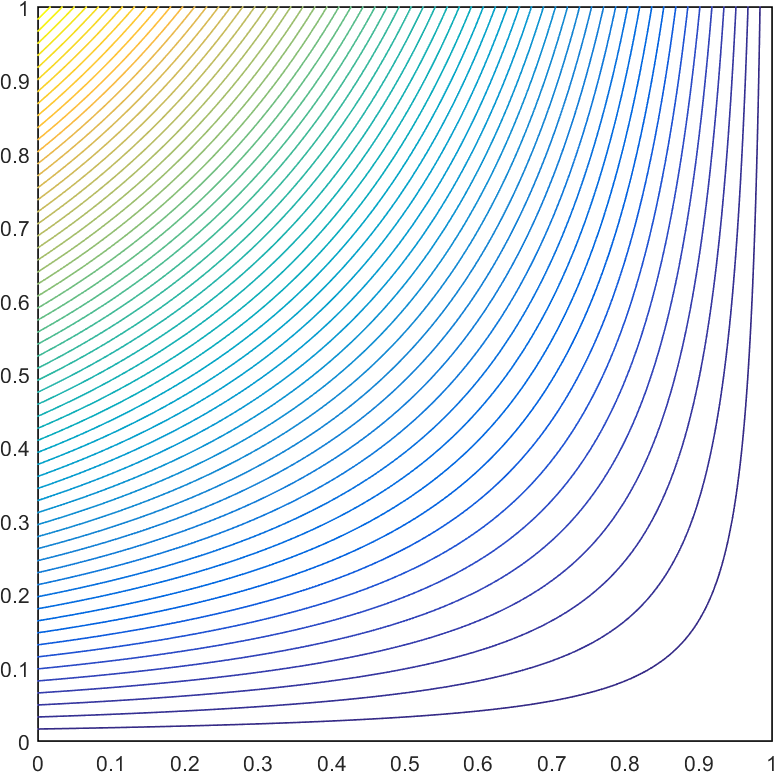
\includegraphics[width=\textwidth]{figures/sec_BF/square_MAXENT1_contour_b4.png}
		\caption{}
	\end{subfigure}
	\hspace{1.5cm}
	\begin{subfigure}[b]{0.39\textwidth}
		\centering
		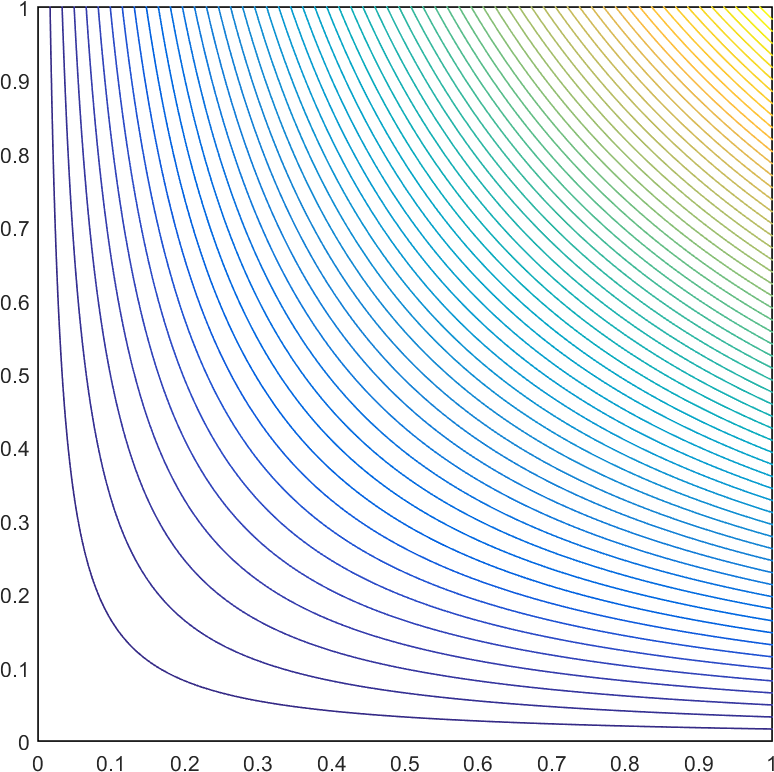
\includegraphics[width=\textwidth]{figures/sec_BF/square_MAXENT1_contour_b3.png}
		\caption{}
	\end{subfigure}
	\vfill
	\begin{subfigure}[b]{0.39\textwidth}
		\centering
		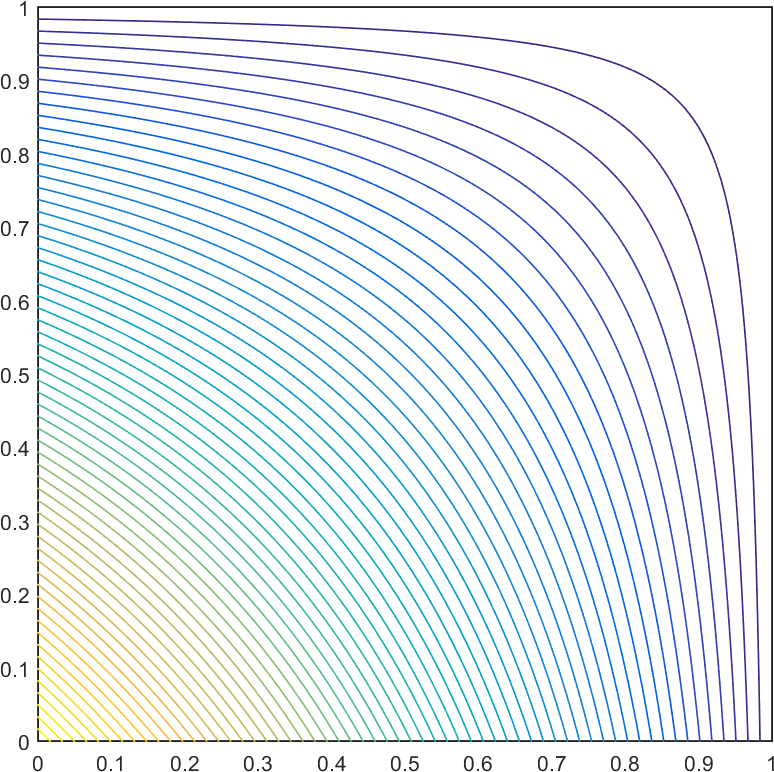
\includegraphics[width=\textwidth]{figures/sec_BF/square_MAXENT1_contour_b1.png}
		\caption{}
	\end{subfigure}
	\hspace{1.5cm}
	\begin{subfigure}[b]{0.39\textwidth}
		\centering
		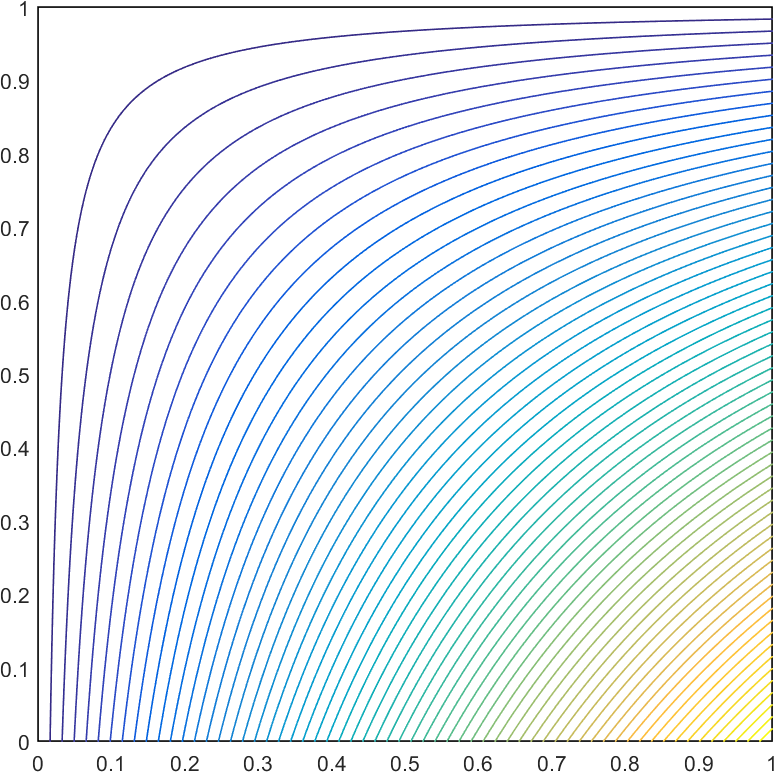
\includegraphics[width=\textwidth]{figures/sec_BF/square_MAXENT1_contour_b2.png}
		\caption{}
	\end{subfigure}
\caption{Contour plots of the linear maximum entropy basis functions on the unit square for the vertices located at: (a) (0,1), (b) (1,1), (c) (0,0), and (d) (1,0).}
\label{fig::2D_MAXENT1_unit_square_basis_functions}
\end{figure}

\begin{figure}
\centering
	\begin{subfigure}[b]{0.39\textwidth}
		\centering
		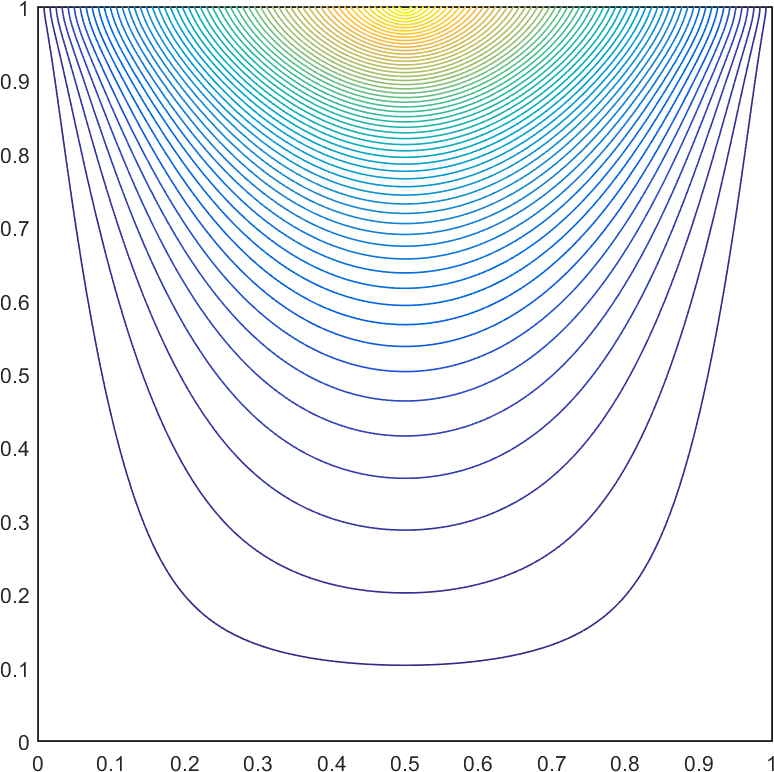
\includegraphics[width=\textwidth]{figures/sec_BF/deg_square_MAXENT1_contour_b4.png}
		\caption{}
	\end{subfigure}
	\vfill
	\begin{subfigure}[b]{0.39\textwidth}
		\centering
		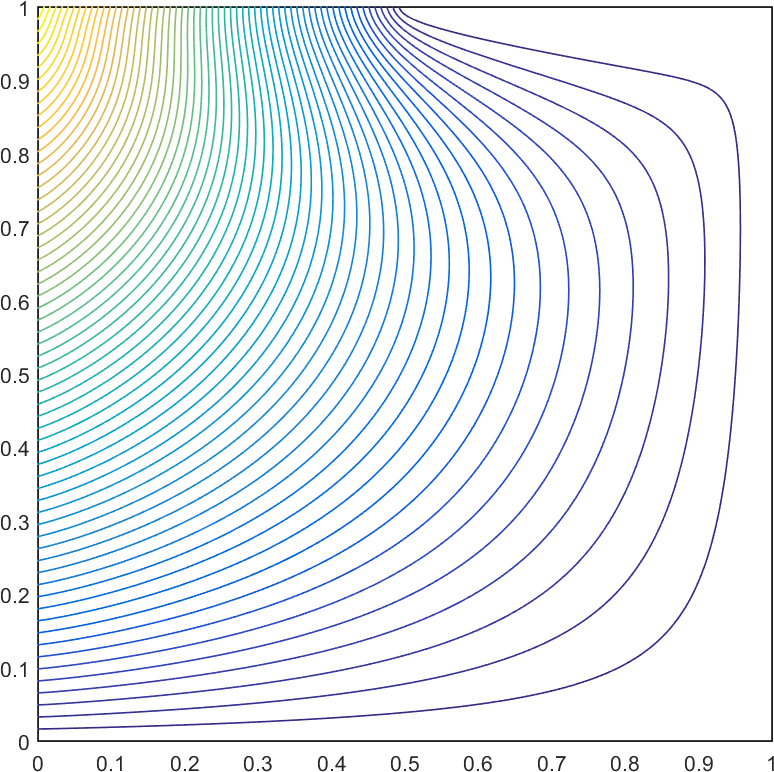
\includegraphics[width=\textwidth]{figures/sec_BF/deg_square_MAXENT1_contour_b5.png}
		\caption{}
	\end{subfigure}
	\hspace{1.5cm}
	\begin{subfigure}[b]{0.39\textwidth}
		\centering
		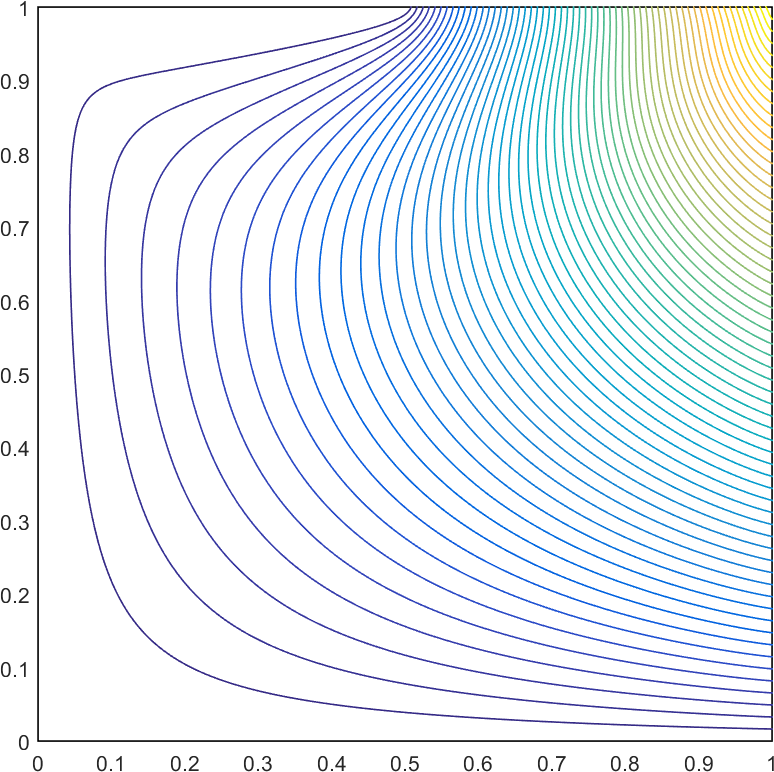
\includegraphics[width=\textwidth]{figures/sec_BF/deg_square_MAXENT1_contour_b3.png}
		\caption{}
	\end{subfigure}
	\vfill
	\begin{subfigure}[b]{0.39\textwidth}
		\centering
		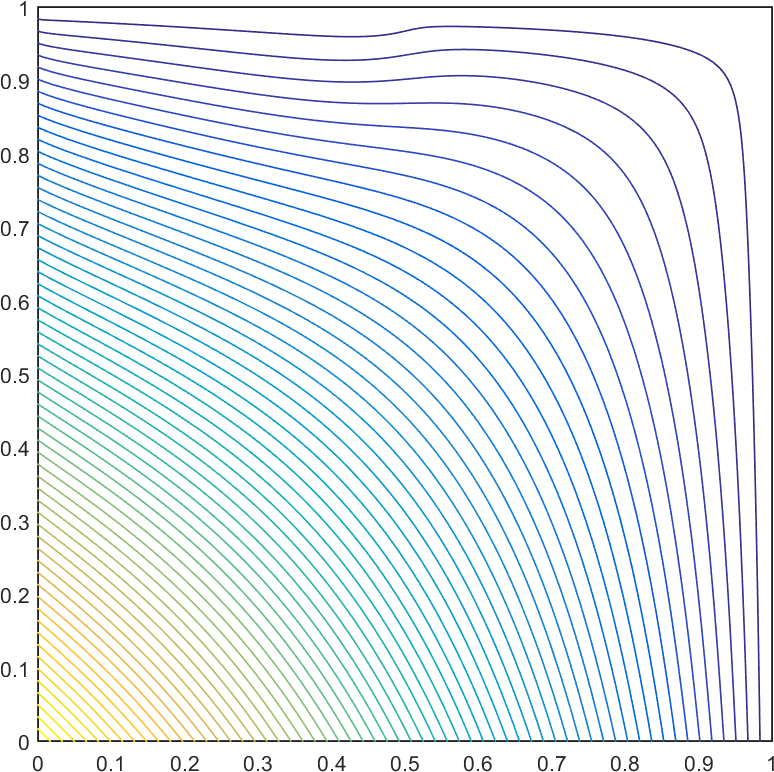
\includegraphics[width=\textwidth]{figures/sec_BF/deg_square_MAXENT1_contour_b1.png}
		\caption{}
	\end{subfigure}
	\hspace{1.5cm}
	\begin{subfigure}[b]{0.39\textwidth}
		\centering
		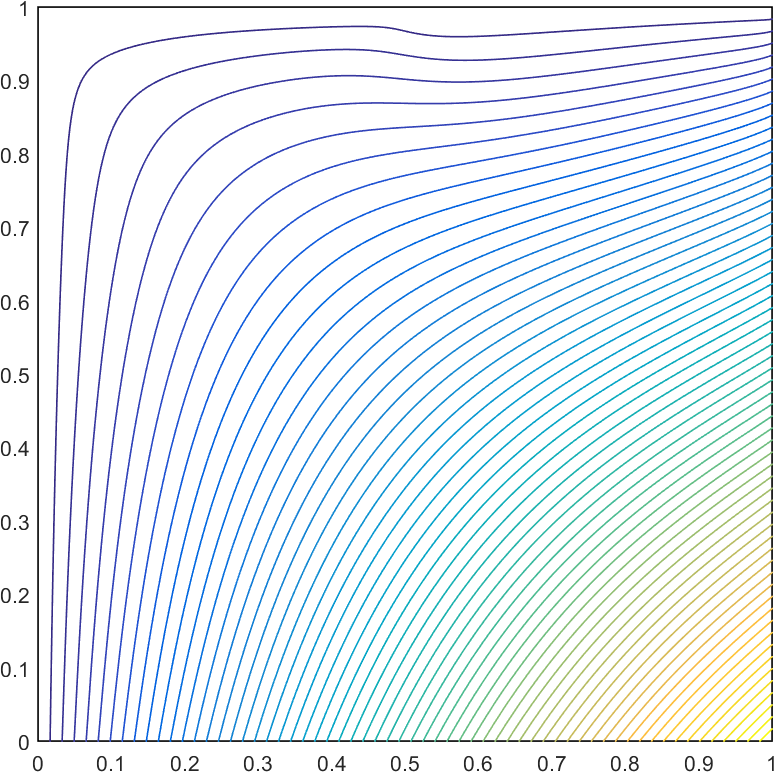
\includegraphics[width=\textwidth]{figures/sec_BF/deg_square_MAXENT1_contour_b2.png}
		\caption{}
	\end{subfigure}
\caption{Contour plots of the linear maximum entropy basis functions on the degenerate pentagon for the vertices located at: (a) (1/2,1), (b) (0,1), (c) (1,1), (d) (0,0), and (e) (1,0).}
\label{fig::2D_MAXENT1_deg_square_basis_functions}
\end{figure}

\begin{figure}
\centering
	\begin{subfigure}[b]{0.39\textwidth}
		\centering
		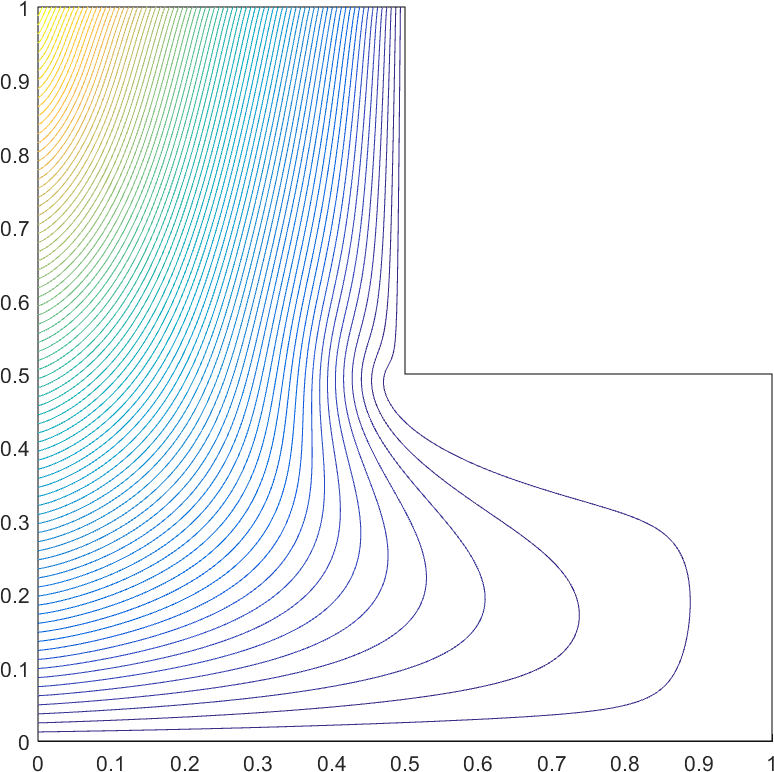
\includegraphics[width=\textwidth]{figures/sec_BF/L-domain_MAXENT1_contour_b6.png}
		\caption{}
	\end{subfigure}
	\hspace{1.5cm}
	\begin{subfigure}[b]{0.39\textwidth}
		\centering
		\includegraphics[width=\textwidth]{figures/sec_BF/L-domain_MAXENT1_contour_b5.png}
		\caption{}
	\end{subfigure}
	\vfill
	\begin{subfigure}[b]{0.39\textwidth}
		\centering
		\includegraphics[width=\textwidth]{figures/sec_BF/L-domain_MAXENT1_contour_b4.png}
		\caption{}
	\end{subfigure}
	\hspace{1.5cm}
	\begin{subfigure}[b]{0.39\textwidth}
		\centering
		\includegraphics[width=\textwidth]{figures/sec_BF/L-domain_MAXENT1_contour_b3.png}
		\caption{}
	\end{subfigure}
	\vfill
	\begin{subfigure}[b]{0.39\textwidth}
		\centering
		\includegraphics[width=\textwidth]{figures/sec_BF/L-domain_MAXENT1_contour_b1.png}
		\caption{}
	\end{subfigure}
	\hspace{1.5cm}
	\begin{subfigure}[b]{0.39\textwidth}
		\centering
		\includegraphics[width=\textwidth]{figures/sec_BF/L-domain_MAXENT1_contour_b2.png}
		\caption{}
	\end{subfigure}
\caption{Contour plots of the linear maximum entropy basis functions on the L-shaped domain for the vertices located at: (a) (0,1), (b) (1/2,1), (c) (1/2,1/2), (d) (1,1/2), (e) (0,0), and (f) (1,0).}
\label{fig::2D_MAXENT1_Ldom_basis_functions}
\end{figure}



%%%%%%%%%%%%%%%%%%%%%%%%%%%%%%%%%%%%%%%%%%%%%%%%%%%
%%%   SubSection - 2D linear summary
\subsection{Summary of 2D Linear Basis Functions on Polygons}
\label{sec::BF_2DLinear_Summary}

In Sections \ref{sec::BF_2DLinear_Wachspress}, \ref{sec::BF_2DLinear_PWL}, \ref{sec::BF_2DLinear_MV}, and \ref{sec::BF_2DLinear_ME}, we presented the linear Wachspress, PWL, mean value, and maximum entropy coordinates, respectively. We gave the functional forms for their values and gradients along with example contour plots for different polygonal elements. Table \ref{tab::BF_2Dlin_summary} provides a summary of the properties for the different coordinates. The Wachspress, PWL, and ME functions have natural extensions to 3D polyhedra, but the MV functions can only interpolate on polyhedra with triangular facets \cite{floater2005mean,wicke2007finite}. The PWL, MV, and ME coordinates can interpolate degenerate-convex and concave polygons while the Wachspress functions can only interpolate strictly-convex polygons. This means that the Wachspress coordinates are not suited for AMR calculations that form degenerate polygons. PWL is the only functional form that can analytically integrate the elementary matrices and directly evaluate its values and gradients on the boundary of the polygon. Finally, every point within the domain can be directly evaluated using the Wachspress, PWL, and MV coordinates. However, the ME coordinates use an iterative approach with Newton's method since their functional form constitutes a non-linear minimization problem.

We conclude this summary discussion on the different linearly-complete 2D polygonal coordinates by again presenting examples of their functional forms. Figure \ref{fig::2D_Linear_Summary_unit_square_basis_functions} provides the contour plots of the different coordinates located at vertex ($0,1$) on the unit square. It is easy to see that the Wachspress, MV, and ME coordinates are smoothly varying within the polygon's domain while the PWL coordinates only have $C^0$ continuity. Figure \ref{fig::2D_Summary_deg_square_basis_functions} provides the contour plots on the degenerate pentagon that is formed by inserting a vertex at $(1/2,1)$ into the unit square. This re-emphasizes that the Wachspress coordinates are only valid interpolatory functions on strongly-convex polygons. Finally, Figure \ref{fig::2DSummary_Ldom_basis_functions} provides the contour plots of the PWL, MV, and ME functions on the L-shaped domain at the $(0,1)$ and $(1/2,1/2)$ vertices. These coordinates can successfully interpolate on concave polygons.

\begin{table}
\centering
\caption[Summary of the 2D polygonal basis functions]{Summary of the properties of the 2D coordinate systems used on polygons. }
\begin{tabular}{|c|c|c|c|c|}
\hline
Basis Function & Dimension & Polygon Type & Integration & Evaluation \\
\hline \hline
Wachspress	&2D/3D&	Convex&	Numerical	&Direct\\ \hline
PWL&	1D/2D/3D&	Convex/Concave&	Analytical	&Direct\\ \hline
Mean Value&	2D&	Convex/Concave&	Numerical	&Direct\\ \hline
Max Entropy&	1D/2D/3D	&Convex/Concave&	Numerical&	Iterative\\ \hline
\end{tabular}
\label{tab::BF_2Dlin_summary}
\end{table}

\begin{figure}
\centering
{
	\begin{subfigure}[b]{0.39\textwidth}
		\centering
		\includegraphics[width=\textwidth]{figures/sec_BF/square_WACHSPRESS1_contour_b4.png}
		\caption{Wachspress}
	\end{subfigure}
	\hspace{1.5cm}
	\begin{subfigure}[b]{0.39\textwidth}
		\centering
		\includegraphics[width=\textwidth]{figures/sec_BF/square_PWLD1_contour_b4.png}
		\caption{PWL}
	\end{subfigure}
}
	\vspace{3mm}
{
	\begin{subfigure}[b]{0.39\textwidth}
		\centering
		\includegraphics[width=\textwidth]{figures/sec_BF/square_MV1_contour_b4.png}
		\caption{Mean Value}
	\end{subfigure}
	\hspace{1.5cm}
	\begin{subfigure}[b]{0.39\textwidth}
		\centering
		\includegraphics[width=\textwidth]{figures/sec_BF/square_MAXENT1_contour_b4.png}
		\caption{Maximum Entropy}
	\end{subfigure}
}
\caption[Contour plots of the linear basis functions on the unit square.]{Contour plots of the different linear basis function on the unit square located at vertex (0,1).}
\label{fig::2D_Linear_Summary_unit_square_basis_functions}
\end{figure}

\begin{figure}
\centering
{
	\begin{subfigure}[b]{0.39\textwidth}
		\centering
		\includegraphics[width=\textwidth]{figures/sec_BF/deg_square_WACHSPRESS1_contour_b5.png}
		\caption{Wachspress}
	\end{subfigure}
	\hspace{1.5cm}
	\begin{subfigure}[b]{0.39\textwidth}
		\centering
		\includegraphics[width=\textwidth]{figures/sec_BF/deg_square_PWLD1_contour_b5.png}
		\caption{PWL}
	\end{subfigure}
}
	\vspace{3mm}
{
	\begin{subfigure}[b]{0.39\textwidth}
		\centering
		\includegraphics[width=\textwidth]{figures/sec_BF/deg_square_MV1_contour_b5.png}
		\caption{Mean Value}
	\end{subfigure}
	\hspace{1.5cm}
	\begin{subfigure}[b]{0.39\textwidth}
		\centering
		\includegraphics[width=\textwidth]{figures/sec_BF/deg_square_MAXENT1_contour_b5.png}
		\caption{Maximum Entropy}
	\end{subfigure}
}
\caption[Contour plots of the linear basis functions on the degenerate pentagon.]{Contour plots of the different linear basis function on the degenerate pentagon located at vertex (0,1). It is clear that the Wachspress coordinates fail for the weakly convex case.}
\label{fig::2D_Summary_deg_square_basis_functions}
\end{figure}

\begin{figure}
\centering
{
	\begin{subfigure}[b]{0.375\textwidth}
		\centering
		\includegraphics[width=\textwidth]{figures/sec_BF/L-domain_PWLD1_contour_b6.png}
	\end{subfigure}
	\hspace{1.5cm}
	\begin{subfigure}[b]{0.375\textwidth}
		\centering
		\includegraphics[width=\textwidth]{figures/sec_BF/L-domain_PWLD1_contour_b4.png}
	\end{subfigure}
}
\vspace{3mm}
{
	\begin{subfigure}[b]{0.375\textwidth}
		\centering
		\includegraphics[width=\textwidth]{figures/sec_BF/L-domain_MV1_contour_b6.png}
	\end{subfigure}
	\hspace{1.5cm}
	\begin{subfigure}[b]{0.375\textwidth}
		\centering
		\includegraphics[width=\textwidth]{figures/sec_BF/L-domain_MV1_contour_b4.png}
	\end{subfigure}
}
\vspace{3mm}
{
	\begin{subfigure}[b]{0.375\textwidth}
		\centering
		\includegraphics[width=\textwidth]{figures/sec_BF/L-domain_MAXENT1_contour_b6.png}
	\end{subfigure}
	\hspace{1.5cm}
	\begin{subfigure}[b]{0.375\textwidth}
		\centering
		\includegraphics[width=\textwidth]{figures/sec_BF/L-domain_MAXENT1_contour_b4.png}
	\end{subfigure}
}
\vspace{2mm}
\caption[Contour plots of the linear basis functions on the L-shaped domain.]{Contour plots of the different linear basis functions on the L-shaped domain. The PWL (top), mean value (middle), and maximum entropy (bottom) functions are plotted at vertices $(0,1)$ (left) and $(1/2,1/2)$ (right).}
\label{fig::2DSummary_Ldom_basis_functions}
\end{figure}

%%%%%%%%%%%%%%%%%%%%%%%%%%%%%%%%%%%%%%%%%%%%%%%%%%%
%%%%%%%%%%%%%%%%%%%%%%%%%%%%%%%%%%%%%%%%%%%%%%%%%%%
%%%
%%%   Section - Quadratic Basis Functions
%%%
%%%%%%%%%%%%%%%%%%%%%%%%%%%%%%%%%%%%%%%%%%%%%%%%%%%
%%%%%%%%%%%%%%%%%%%%%%%%%%%%%%%%%%%%%%%%%%%%%%%%%%%
\section{Converting the Linear Polygonal Basis Functions to the Quadratic Serendipity Space of Functions}
\label{sec::BF_2DQuadratic}

We have given complete details on the linearly-complete generalized barycentric coordinates that we will investigate for this work. Now we describe how to convert any generalized barycentric coordinate into the quadratic serendipity space of functions to yield quadratic (not linear) precision based on the work of Rand et al. \cite{rand2014quadratic}. The maximum entropy coordinates were independently converted into the quadratic space \cite{gonzalez2010higher,sukumar2013quadratic}. These 2D serendipity coordinates can exactly interpolate the $\{ 1, x, y, x^2, xy, y^2 \}$ span of functions, which can be shown with the first three levels of Pascal's triangle:

\begin{equation}
\label{eq::BF_quad_pascal}
\begin{array}{ccccc}
 & & 1 & & \\
 & x & & y & \\
 x^2 &  &xy & & y^2 
\end{array} \, 
\end{equation}

\noindent Between the linear and quadratic precision of the generalized barycentric coordinates and the quadratic serendipity extension, a relation can be formed on the functional space of their precision. If we seek a functional space up to order $p$ precision, then for $k=0,...,p$, the interpolatory functions must exactly span the following monomial functions,

\begin{equation}
\label{eq::BF_quad_monomial}
f_{\sigma, \tau}^k (x, y) = x^{\sigma} y^{\tau} ,
\end{equation}

\noindent where $\sigma + \tau = k$. From the first three levels of Pascal's triangle given in Eq. (\ref{eq::BF_quad_pascal}), we see that $k=0$ gives the constant function $\{ 1 \}$, that $k=1$ gives the linear functions $\{ x,y \}$, and that $k=2$ gives the quadratic functions $\{ x^2,xy,y^2 \}$.

\begin{figure}[hbt]
\centering
\includegraphics[width=\textwidth]{figures/sec_BF/linear_to_quad_process.png}
\caption{Overview of the process to construct the quadratic serendipity basis functions on polygons. The filled dots correspond to basis functions that maintain the Lagrange property while empty dots do not.}
\label{fig::BF_2D_quad_process}
\end{figure}

Now, we give the full details on converting the linear generalized barycentric coordinates to the quadratic serendipity space of functions. Figure \ref{fig::BF_2D_quad_process} gives a visual depiction of this conversion process. For a polygon with $N_K$ vertices, we can summarize this procedure as the following:

\begin{enumerate}
\item For a point $\vec{x}$, compute the $N_K$ linear barycentric functions $\{ \lambda_i (\vec{x}) \}$ (Wachspress, PWL, mean value, or maximum entropy);
\item Take all non-repeating pairwise products of the linear functions to obtain $\frac{N_K(N_K+1)}{2}$ quadratic functions $\{ \mu_{ab} \}$;
\item Form the linear transformation matrix $\mathbb{A}$ through the use of monomial constraint equations;
\item Use the $\mathbb{A}$ matrix to reduce the $\{ \mu_{ab} \}$ function set to the $2 N_K$ serendipity basis set $\{ \xi_{ij} \}$.
\end{enumerate}

We begin by computing the ($i=1,...,N_K$) linear barycentric functions, $\{ \lambda_i (\vec{x}) \}$, and their gradients, $\{ \vec{\nabla} \lambda_i (\vec{x}) \}$, for a point $\vec{x}$. These linearly-complete barycentric functions can be converted immediately to barycentric-like functions with quadratic precision. Taking all non-repeating pairwise products of the linear functions yields a total of $N_Q=\frac{N_K(N_K+1)}{2}$ quadratic functions: $\mu_{ab} = \lambda_a \lambda_b$. Doing this generates functions that either live on the polygon's vertices, mid-face points, or midpoints of the polygon's diagonals between two vertices as seen in Figure \ref{fig::BF_2D_quad_process}. The $N_K$ vertex functions are denoted as $ab \in V$, the $N_K$ mid-face functions are denoted as $ab \in E$, and the $\frac{N_K(N_K-3)}{2}$ diameter functions are denoted as $ab \in D$. We also define the abbreviated notation of $\vec{x}_{ab} = \frac{\vec{x}_a + \vec{x}_b}{2}$, so that $\vec{x}_{aa}$ corresponds to a vertex function at $\vec{x}_a$. Using these various notations, we can write the precision properties of the $\mu_{ab}$ functions for the constant constraint,

\begin{equation}
\label{eq::BF_quad_interp_req_constant_alt}
\sum_{aa \in V}  \mu_{aa} (\vec{x}) + \sum_{ab \in E \cup D} 2 \mu_{ab} (\vec{x})  = 1 ,
\end{equation}

\noindent for the linear constraint,

\begin{equation}
\label{eq::BF_quad_interp_req_linear_alt}
\sum_{aa \in V}  \mu_{aa} (\vec{x}) \, \vec{x}_{aa} +  \sum_{ab \in E \cup D} 2  \mu_{ab} (\vec{x}) \, \vec{x}_{ab} = \vec{x} ,
\end{equation}

\noindent and for the quadratic constraint,

\begin{equation}
\label{eq::BF_quad_interp_req_quadratic_alt}
\sum_{aa \in V}  \mu_{aa} (\vec{x}) \, \left( \vec{x}_a \otimes \vec{x}_a \right) +  \sum_{ab \in E \cup D}   \mu_{ab} (\vec{x}) \, \left( \vec{x}_a \otimes \vec{x}_b + \vec{x}_b \otimes \vec{x}_a \right)   =  \vec{x} \otimes \vec{x} .
\end{equation}


\noindent In Eq. (\ref{eq::BF_quad_interp_req_quadratic_alt}), $\otimes$ is the dyadic tensor product. We can immediately see that quadratic precision is ensured. However, the set of these pairwise quadratic functions grows quadratically. This means that as $N_K$ grows large, the number of interpolatory functions grows as order $O(N_K^2)$, but still only maintains precision of the $\{ 1, x, y, x^2, xy, y^2 \}$ span of functions. Therefore, the computational work required to utilize these quadratic barycentric functions can become prohibitive for polygons with large vertex counts.

To minimize the number of interpolatory functions but still maintain the precision of the $\{ 1, x, y, x^2, xy, y^2 \}$ span of functions, we seek to convert the quadratic barycentric functions into the quadratic serendipity space of functions $\{ \xi_{ij} \}$. This quadratic serendipity space only contains the vertex and mid-face functions (total of $2 N_K$) and has been extensively studied for tensor-based elements in the past \cite{macneal1992eight,arnold2011serendipity}. This means that we seek to reduce the $\{ \mu_{ab} \}$ set of functions by removing the diagonal functions ($ab \in D$) while still maintaining quadratic precision. If we define $\xi_{ii}$ and $\xi_{i(i+1)}$ as the serendipity functions that live at vertex $i$ and the mid-face point between vertices $i$ and $i+1$, respectively, then we can write the serendipity precision properties for the constant constraint,

\begin{equation}
\label{eq::BF_ser_interp_req_constant}
\sum_{ii \in V}  \xi_{ii} (\vec{x}) + \sum_{i(i+1) \in E} 2 \xi_{i(i+1)} (\vec{x})  = 1 ,
\end{equation}

\noindent for the linear constraint,

\begin{equation}
\label{eq::BF_ser_interp_req_linear}
\sum_{ii \in V}  \xi_{ii} (\vec{x}) \, \vec{x}_{ii} +  \sum_{i(i+1) \in E} 2  \xi_{i(i+1)} (\vec{x}) \, \vec{x}_{i(i+1)} = \vec{x} ,
\end{equation}

\noindent and for the quadratic constraint,

\begin{equation}
\label{eq::BF_ser_interp_req_quadratic}
\sum_{ii \in V}  \xi_{ii} (\vec{x}) \, \left( \vec{x}_i \otimes \vec{x}_i \right) +  \sum_{i(i+1) \in E}   \xi_{i(i+1)} (\vec{x}) \, \left( \vec{x}_i \otimes \vec{x}_{i+1} + \vec{x}_{i+1} \otimes \vec{x}_i \right)   =  \vec{x} \otimes \vec{x} .
\end{equation}

To remove the diagonal functions, we formalize this procedure by recasting it as a linear algebra problem. We seek a matrix $\mathbb{A}$ such that the linear transformation, 

\begin{equation}
\label{eq::BF_quad_to_ser_mapping}
\left\{ \xi \right\} = \mathbb{A} \left\{ \mu \right\} ,
\end{equation}

\noindent will satisfy the precision properties of Eqs. (\ref{eq::BF_ser_interp_req_constant} - \ref{eq::BF_ser_interp_req_quadratic}). It is easy to see that $\mathbb{A}$ has dimension ($2 N_K \times N_Q$). We wish for this matrix to have constant entries for any point within the polygon's interior so that it does not have to be recalculated for each interpolatory point of interest. To ease the notation, we will assign specific basis orderings for the quadratic and quadratic serendipity functions. The serendipity basis is ordered such that all vertex functions ($ii \in V$) in a counter-clockwise ordering are first, followed by a counter-clockwise ordering of the mid-face nodes ($ij \in E$) starting with the node between vertices 1 and 2. This ordering can be succinctly stated by

\begin{equation}
\label{eq::BF_ser_ordering}
\left\{ \xi_{ij} \right\} = \Big\{ \left[  \xi_{11}, \xi_{22}, ... , \xi_{N_K N_K} \right] , \left[ \xi_{12}, \xi_{23}, ..., \xi_{(N_K-1)N_K}, \xi_{N_K(N_K+1)} \right] \Big\} .
\end{equation}

\noindent The quadratic basis begins identically to the serendipity basis by first listing the vertex and mid-face functions. Then the diagonal functions are indexed in lexicographical order. This gives the following ordering for the quadratic functions

\begin{equation}
\label{eq::BF_quad_ordering}
\begin{aligned}
\left\{ \mu_{ab} \right\} = \Big\{ \left[  \mu_{11}, \mu_{22}, ... , \mu_{N_K N_K} \right] , &\left[ \mu_{12}, \mu_{23}, ..., \mu_{(N_K-1)N_K}, \mu_{N_K(N_K+1)} \right] ,\\ 
&\left[ \mu_{13}, ..., \text{(lexicographical)} ,..., \mu_{(N_K-2)N_K} \right] \Big\} 
\end{aligned} .
\end{equation}

\noindent With these basis orderings, we can now denote the entries of $\mathbb{A}$ (given by $c_{ab}^{ij}$) as the following:

\begin{equation}
\label{eq::BF_quad_to_ser_matrix_constraints}
\mathbb{A} = 
\left[
\begin{array}{ccccc}
c_{11}^{11} & \ldots & c_{ab}^{11} & \ldots & c_{(n-2)n}^{11} \\
\ldots&\ddots&\vdots&\ddots&\vdots \\
c_{11}^{ij} & \ldots & c_{ab}^{ij} & \ldots & c_{(n-2)n}^{ij} \\
\ldots&\ddots&\vdots&\ddots&\vdots \\
c_{11}^{n(n+1)} & \ldots & c_{ab}^{n(n+1)} & \ldots & c_{(n-2)n}^{n(n+1)} 
\end{array}
\right] .
\end{equation}

A sufficient set of constraints for the entries in $\mathbb{A}$ to ensure the precision properties of Eqs. (\ref{eq::BF_ser_interp_req_constant} - \ref{eq::BF_ser_interp_req_quadratic}) can be written for the constant constraint,

\begin{equation}
\label{eq::BF_Amat_cons_constraints}
\begin{aligned}
\sum_{ii \in V} c_{aa}^{ii} + \sum_{i(i+1) \in E} 2 c_{aa}^{i(i+1)} = 1, &\qquad \forall aa \in V \\
\sum_{ii \in V} c_{ab}^{ii} + \sum_{i(i+1) \in E} 2 c_{ab}^{i(i+1)} = 2, &\qquad \forall ab \in E \cup D
\end{aligned}
\end{equation}

\noindent for the linear constraint,

\begin{equation}
\label{eq::BF_Amat_lin_constraints}
\begin{aligned}
\sum_{ii \in V} c_{aa}^{ii} \vec{x}_{ii} + \sum_{i(i+1) \in E} 2 c_{aa}^{i(i+1)} \vec{x}_{i(i+1)} = \vec{x}_{aa}, &\qquad \forall aa \in V \\
\sum_{ii \in V} c_{ab}^{ii} \vec{x}_{ii} + \sum_{i(i+1) \in E} 2 c_{ab}^{i(i+1)} \vec{x}_{i(i+1)} = 2 \vec{x}_{ab}, &\qquad \forall ab \in E \cup D
\end{aligned}
\end{equation}

\noindent for the $a\in V$ vertex quadratic constraints

\begin{equation}
\label{eq::BF_Amat_quad_vert_constraints}
\sum_{ii \in V} c_{aa}^{ii} \vec{x}_{ii} \otimes \vec{x}_{ii} + \sum_{i(i+1) \in E}  c_{aa}^{i(i+1)} \left( \vec{x}_i \otimes \vec{x}_{i+1} + \vec{x}_{i+1} \otimes \vec{x}_i \right) = \vec{x}_{aa} \otimes \vec{x}_{aa}, 
\end{equation}

\noindent and for the $ab \in E \cup D$ mid-face and diagonal quadratic constraints,

\begin{equation}
\label{eq::BF_Amat_quad_facediag_constraints}
\sum_{ii \in V} c_{ab}^{ii} \vec{x}_{ii} \otimes \vec{x}_{ii} + \sum_{i(i+1) \in E}  c_{ab}^{i(i+1)} \left( \vec{x}_i \otimes \vec{x}_{i+1} + \vec{x}_{i+1} \otimes \vec{x}_i \right) = \left( \vec{x}_a \otimes \vec{x}_{b} + \vec{x}_{b} \otimes \vec{x}_a \right).
\end{equation}

\noindent For $N_K > 3$, there are more coefficients than the six constraint equations. This means that there is flexibility in the construction of the solution to the constraint equations. Therefore, we choose a simple structure for $\mathbb{A}$ that consists of the following,


\begin{equation}
\label{eq::BF_quad_Amat_simple}
\mathbb{A} = \left[ \mathbb{I} \, | \, \mathbb{A}' \right],
\end{equation}

\noindent where $\mathbb{I}$ is the ($2 N_K \text{x} 2 N_K$) identity matrix, and $\mathbb{A}'$ is a full ($2 N_K \text{x}  \frac{N_K(N_K-3)}{2}$) matrix. This means that the vertex and face midpoint serendipity functions, $\xi_{ij}$, are formed by taking their corresponding quadratic function, $\mu_{ij}$, and adding some linear combination of the interior functions. Therefore, we only need to determine the $\frac{N_K(N_K-3)}{2}$ columns of the $\mathbb{A}'$ matrix to complete this linear transformation. 

In their work, Rand et al. proposed a methodology where only six coefficients are chosen to be non-zero and can be directly calculated through geometric expressions. However, their approach is only valid for strictly-convex polygons. This will not work for our analysis since we wish to also analyze degenerate polygons that will arise in our AMR calculations. Therefore, we will use a least squares method to calculate each of the columns of $\mathbb{A}'$. We note that the coefficients calculated with this least squares method and that of Rand will be identical only for orthogonal quadrilaterals. If we isolate the column $(ab)$ from $\mathbb{A}'$, then we can form the following system of equations, 

\begin{equation}
\label{eq::BF_quad_MP_form}
\mathbb{B} \vec{c}_{ab} = \vec{q}_{ab}, 
\end{equation}

\noindent where $\mathbb{B}$ is a matrix of dimension $(6 \text{x} 2 N_K)$, $\vec{c}_{ab}$ is vector of length $2 N_K$, and $\vec{q}_{ab}$ is a vector of length 6. The entries of $\mathbb{B}$ correspond to coefficients given in the left-hand-side terms of Eqs. (\ref{eq::BF_Amat_cons_constraints}), (\ref{eq::BF_Amat_lin_constraints}), and (\ref{eq::BF_Amat_quad_facediag_constraints}). The values of $\vec{q}_{ab}$ are given by the right-hand-side constants of these same equations. To invert $\mathbb{B}$, we use the Moore-Penrose pseudoinverse (denoted as $\mathbb{B}^*$) \cite{penrose1955generalized}. For an under-determined system of equations, the pseudoinverse is given by,

\begin{equation}
\label{eq::BF_quad_MP_inverse}
\mathbb{B}^* = \mathbb{B}^T (\mathbb{B} \mathbb{B}^T)^{-1}.
\end{equation}

\noindent Once all of the coefficients for the $\mathbb{A}'$ matrix are known, each of the quadratic serendipity functions can be computed by

\begin{equation}
\label{eq::BF_quad_xi_reduced}
\begin{aligned}
\xi_{ij} &=  \mu_{i,j} + \sum_{ab \in D} c_{ab}^{ij} \mu_{ab} \\
&=  \lambda_i \lambda_j + \sum_{ab \in D} c_{ab}^{ij}\lambda_a \lambda_b
\end{aligned} .
\end{equation}

The gradients of the serendipity basis are simple to compute with the chain rule of Calculus. If we take the gradient of Eq. (\ref{eq::BF_quad_xi_reduced}) and use appropriate derivative rules, then the gradients of the different serendipity functions can be given by

\begin{equation}
\label{eq::BF_ser_gradient}
\vec{\nabla} \xi_{ij} = \lambda_j \vec{\nabla} \lambda_i + \lambda_i \vec{\nabla} \lambda_j + \sum_{ab \in D} c_{ab}^{ij} \left(  \lambda_b \vec{\nabla} \lambda_a + \lambda_a \vec{\nabla} \lambda_b \right) .
\end{equation}

\noindent This means that all of the serendipity basis function gradients can be computed from the appropriate values and gradients of the linear barycentric basis functions using the linear transformation of the $\mathbb{A}$ matrix.

We now present some example contour plots for the conversion of the linear barycentric coordinates into the quadratic serendipity space. Figures \ref{fig::2D_Quadratic_Summary_unit_square_basis_functions_BF4} and \ref{fig::2D_Quadratic_Summary_unit_square_basis_functions_BF8} provide the contour plots of the different quadratic serendipity functions located at the upper-left vertex and left side-node, respectively. Then, Figure \ref{fig::2DQuadSer_degsquare_basis_functions} provides some of the contour plots of the PWL, MV, and ME basis functions on the degenerate square that is formed by inserting a vertex at ($1/2,1$) onto the unit square.

\begin{figure}
\centering
	\begin{subfigure}[b]{0.39\textwidth}
		\centering
		\includegraphics[width=\textwidth]{figures/sec_BF/square_WACHSPRESS2_contour_b4.png}
		\caption{Wachspress}
	\end{subfigure}
	\hspace{1.5cm}
	\begin{subfigure}[b]{0.39\textwidth}
		\centering
		\includegraphics[width=\textwidth]{figures/sec_BF/square_PWLD2_contour_b4.png}
		\caption{PWL}
	\end{subfigure}
	\vfill
	\begin{subfigure}[b]{0.39\textwidth}
		\centering
		\includegraphics[width=\textwidth]{figures/sec_BF/square_MV2_contour_b4.png}
		\caption{Mean Value}
	\end{subfigure}
	\hspace{1.5cm}
	\begin{subfigure}[b]{0.39\textwidth}
		\centering
		\includegraphics[width=\textwidth]{figures/sec_BF/square_MAXENT2_contour_b4.png}
		\caption{Maximum Entropy}
	\end{subfigure}
\caption[Contour plots of the quadratic basis functions on the unit square.]{Contour plots of the different quadratic serendipity basis function on the unit square located at vertex (0,1).}
\label{fig::2D_Quadratic_Summary_unit_square_basis_functions_BF4}
\end{figure}

\begin{figure}
\centering
	\begin{subfigure}[b]{0.39\textwidth}
		\centering
		\includegraphics[width=\textwidth]{figures/sec_BF/square_WACHSPRESS2_contour_b8.png}
		\caption{Wachspress}
	\end{subfigure}
	\hspace{1.5cm}
	\begin{subfigure}[b]{0.39\textwidth}
		\centering
		\includegraphics[width=\textwidth]{figures/sec_BF/square_PWLD2_contour_b8.png}
		\caption{PWL}
	\end{subfigure}
	\vfill
	\begin{subfigure}[b]{0.39\textwidth}
		\centering
		\includegraphics[width=\textwidth]{figures/sec_BF/square_MV2_contour_b8.png}
		\caption{Mean Value}
	\end{subfigure}
	\hspace{1.5cm}
	\begin{subfigure}[b]{0.39\textwidth}
		\centering
		\includegraphics[width=\textwidth]{figures/sec_BF/square_MAXENT2_contour_b8.png}
		\caption{Maximum Entropy}
	\end{subfigure}
\caption[Contour plots of the quadratic basis functions on the unit square.]{Contour plots of the different quadratic serendipity basis function on the unit square at a mid-face node located at (0,1/2).}
\label{fig::2D_Quadratic_Summary_unit_square_basis_functions_BF8}
\end{figure}


\begin{figure}
\centering
{
	\begin{subfigure}[b]{0.375\textwidth}
		\centering
		\includegraphics[width=\textwidth]{figures/sec_BF/deg_square_PWLD2_contour_b5.png}
	\end{subfigure}
	\hspace{1.5cm}
	\begin{subfigure}[b]{0.375\textwidth}
		\centering
		\includegraphics[width=\textwidth]{figures/sec_BF/deg_square_PWLD2_contour_b9.png}
	\end{subfigure}
}
\vspace{3mm}
{
	\begin{subfigure}[b]{0.375\textwidth}
		\centering
		\includegraphics[width=\textwidth]{figures/sec_BF/deg_square_MV2_contour_b5.png}
	\end{subfigure}
	\hspace{1.5cm}
	\begin{subfigure}[b]{0.375\textwidth}
		\centering
		\includegraphics[width=\textwidth]{figures/sec_BF/deg_square_MV2_contour_b9.png}
	\end{subfigure}
}
\vspace{3mm}
{
	\begin{subfigure}[b]{0.375\textwidth}
		\centering
		\includegraphics[width=\textwidth]{figures/sec_BF/deg_square_MAXENT2_contour_b5.png}
	\end{subfigure}
	\hspace{1.5cm}
	\begin{subfigure}[b]{0.375\textwidth}
		\centering
		\includegraphics[width=\textwidth]{figures/sec_BF/deg_square_MAXENT2_contour_b9.png}
	\end{subfigure}
}
\vspace{2mm}
\caption[Contour plots of the quadratic basis functions on the degenerate square.]{Contour plots of the different quadratic serendipity basis functions on the degenerate square. The PWL (top), mean value (middle), and maximum entropy (bottom) functions are plotted at vertices $(0,1)$ (left) and $(1/2,1)$ (right)}
\label{fig::2DQuadSer_degsquare_basis_functions}
\end{figure}


%%%%%%%%%%%%%%%%%%%%%%%%%%%%%%%%%%%%%%%%%%%%%%%%%%%
%%%   Section - Integrating 2D Polygons
\section{Integrating the Arbitrary 2D Polygonal Elements}
\label{sec::BF_2DIntegration}

Sections \ref{sec::BF_2DLinear} and \ref{sec::BF_2DQuadratic} detail how the basis functions and their gradients can be computed at different points on a 2D polygonal element. These basis functions and gradients can then be used to calculate the integrals of the elementary matrices for a given element $K$ as described in Section \ref{sec::Sn_Spatial}. Because the elementary matrix integrals using the Wachspress, mean value, and maximum entropy coordinates cannot be performed analytically, we need to define a numerical quadrature scheme. The spatial quadrature sets need to be amenable to arbitrary polygons and also integrate polynomials exactly (the different polynomial orders of the basis functions). Efficient quadrature schemes exist for both triangles and quadrilaterals \cite{silvester1970symmetric,dunavant1985high,wandzurat2003symmetric,lyness1994survey,cools1987construction}. These include symmetric rules on triangles and cubature and tensor-product rules on triangles and quadrilaterals, respectively. However, polygons have an infinite number of topological shapes and explicit quadrature rules cannot be defined. Because of this, the development of efficient quadrature rules for arbitrary polytopes is an ongoing field of research \cite{nooijen1990symmetric,dasgupta2003integration,mousavi2010generalized}.

At this time, we are only interested in the accuracy and not the efficiency of the integration of the elementary matrices. Therefore, we simply choose to use a simple triangulation-based scheme. The global polygonal element $K$ with $N_K$ vertices is sub-divided into $N_K$ separate triangles. Each of these triangles is formed from two adjacent vertices and the polygon's centroid, $\vec{c}$. For convex and degenerate (not concave) polygons, the centroid can be the average of the vertex coordinates, which is simply given by,

\begin{equation}
\label{eq::BF_2DInt_centroid}
\vec{c} = \frac{1}{N_K} \sum_{i=1}^{N_K} \vec{x}_i .
\end{equation}

\begin{figure}
\centering
\includegraphics[width=0.75\textwidth]{figures/sec_BF/triangle_mapping_Rev1.png}
\caption{Mapping a point on the reference triangle onto a sub-triangle of an arbitrary polygon.}
\label{fig::BF_2D_tri_mapping}
\end{figure}

\noindent Then for each sub-triangle, a quadrature rule with $N_q$ nodes is employed (we do not vary the number of nodes between sub-triangles). This quadrature rule is specified in the reference space of $\{ r, s\}$ on the unit triangle with vertices of (0,0), (1,0), and (0,1). We have chosen a symmetric reference quadrature set that is well documented in the literature \cite{dunavant1985high}. We denote this reference quadrature rule by $\Big\{ \hat{x}_q, \hat{w}_q \Big\}_{q=1}^{N_q}$, where the symbol $\hat{}$ denotes any quantity that lives in the reference space. We note that the sum of the reference weights equals the reference triangle area of 1/2. This reference quadrature is mapped into the global space of the sub-triangle by an affine transformation. The mapping of a point from the reference space, $\hat{{\bf p}}$, to its corresponding point in global space, ${\bf p}$, is done with,

\begin{equation}
\label{eq::BF_2DInt_ref_to_glob}
{\bf p} = {\bf x}_0 + J \hat{{\bf p}} ,
\end{equation}

\noindent where ${\bf x}_0$ is the global position of one of the sub-triangle vertices and $J$ is the Jacobian matrix of the transformation. This mapping is presented graphically in Figure \ref{fig::BF_2D_tri_mapping}. If the global positions of the sub-triangle vertices are given by $\vec{x}_0$, $\vec{x}_1$, and $\vec{x}_2$, then the Jacobian is given by the following, 

\begin{equation}
\label{eq::BF_2DInt_jacobian}
 J = \left[
 \begin{array}{cc}
 x_1 - x_0 & x_2 - x_0 \\
 y_1 - y_0  & y_2 - y_0
 \end{array}
 \right] \, .
\end{equation}

\noindent The Jacobian matrix can also be used to map the gradients between the reference and global spaces. The gradient of the reference space can be computed in terms of the global space by,

\begin{equation}
\label{eq::BF_2DInt_grad_ref}
\nabla_{\hat{x}} = J^{T} \nabla_{x}  ,
\end{equation}

\noindent and the gradient of the global space can be computed in terms of the reference space by,

\begin{equation}
\label{eq::BF_2DInt_grad_glob}
\nabla_{x} = J^{-T} \nabla_{\hat{x}}  
\end{equation}

With the positions of the nodes mapped to the global space, that just leaves the weights. The value of the global weight $q$ on sub-triangle $i$ within polygon $K$ (given by $w_{i,q}^K$) is mapped from the corresponding reference weight, $\hat{w}_q$, by

\begin{equation}
\label{eq::BF_2DInt_ref_to_glob_wt}
w_{i,q}^K =   \hat{w}_q | J_i | .
\end{equation}

\noindent In Eq. (\ref{eq::BF_2DInt_ref_to_glob_wt}), $| J_i |$ is the determinant of the Jacobian matrix corresponding to the transformation of sub-triangle $i$, and it is equal to 2 times the area of the sub-triangle $i$. This means that the determinant acts to normalize the weights so that their sum is equal to the sub-triangle's area. Therefore, summing all the weights of all of the sub-triangles will equal the total area of the polygon $K$.

To this point, we have provided the means to generate the quadrature nodes and weights within the global space of a polygon $K$. Next, the values and gradients of the basis functions at these quadrature nodes can be calculated by the procedures outlined in Sections \ref{sec::BF_2DLinear} and \ref{sec::BF_2DQuadratic}. Then, the function $f$ can be integrated over the polygon $K$ by the double sum,

\begin{equation}
\label{eq::BF_2DIntegration_cellK}
\int\displaylimits_{K} f = \sum_{i=1}^{N_K} \sum_{q=1}^{N_q} w_{i,q}^K f (\vec{x}_{i,q}) ,
\end{equation}

\noindent where $w_{i,q}^K$ and $\vec{x}_{i,q}$ correspond to the quadrature weights and global positions for node $q$ within sub-triangle $i$, respectively. In this case, the function $f$ can either be some scalar quantity or an elementary matrix. Thus, the elementary matrices needed for the DGFEM formulation of the transport equation can be computed in a logical manner for any arbitrary polygon. In a similar manner, the integral of $f$ over the entire mesh, $\mathbb{T}_h$, is simply the sum of integrals over all elements. This integration of $f$ over the entire domain is simply given by

\begin{equation}
\label{eq::BF_2DIntegration_domain}
\int\displaylimits_{\mathbb{T}_h} f = \sum_{K \in \mathbb{T}_h} \left( \sum_{i=1}^{N_K} \sum_{q=1}^{N_q} w_{i,q}^K f (\vec{x}_{i,q}) \right) ,
\end{equation}

\noindent which is clearly just an element-wise sum of Eq. (\ref{eq::BF_2DIntegration_cellK}).

We conclude this section by providing some visual examples of quadrature sets for polygonal elements. Figure \ref{fig::BF_2DIntegration_RefTri} gives quadrature sets on the reference triangle for orders 1-6 \cite{dunavant1985high}. We can see that our reference quadrature is symmetric about any of the three vertices, though we note that true isoparametric symmetry is only obtained with equilateral triangles. Then Figures \ref{fig::BF_2DIntegration_Pentagon} and \ref{fig::BF_2DIntegration_Hexagon} provide examples of the mapping of the reference quadrature into the global space for a regular pentagon and hexagon, respectively. 

\begin{figure}
\centering
{
	\begin{subfigure}[b]{0.475\textwidth}
		\centering
		\label{subfig::2DInt_RefTri_Q1}
		\includegraphics[width=0.75\textwidth]{figures/sec_BF/RefTriQuad_Q1.eps}
		\caption{Order 1}
	\end{subfigure}
	\hfill
	\begin{subfigure}[b]{0.475\textwidth}
		\centering
		\label{subfig::2DInt_RefTri_Q2}
		\includegraphics[width=0.75\textwidth]{figures/sec_BF/RefTriQuad_Q2.eps}
		\caption{Order 2}
	\end{subfigure}
}
\vspace{3mm}
{
	\begin{subfigure}[b]{0.475\textwidth}
		\centering
		\label{subfig::2DInt_RefTri_Q3}
		\includegraphics[width=0.75\textwidth]{figures/sec_BF/RefTriQuad_Q3.eps}
		\caption{Order 3}
	\end{subfigure}
	\hfill
	\begin{subfigure}[b]{0.475\textwidth}
		\centering
		\label{subfig::2DInt_RefTri_Q4}
		\includegraphics[width=0.75\textwidth]{figures/sec_BF/RefTriQuad_Q4.eps}
		\caption{Order 4}
	\end{subfigure}
}
\vspace{3mm}
{
	\begin{subfigure}[b]{0.475\textwidth}
		\centering
		\label{subfig::2DInt_RefTri_Q5}
		\includegraphics[width=0.75\textwidth]{figures/sec_BF/RefTriQuad_Q5.eps}
		\caption{Order 5}
	\end{subfigure}
	\hfill
	\begin{subfigure}[b]{0.475\textwidth}
		\centering
		\label{subfig::2DInt_RefTri_Q6}
		\includegraphics[width=0.75\textwidth]{figures/sec_BF/RefTriQuad_Q6.eps}
		\caption{Order 6}
	\end{subfigure}
}
\caption{Quadrature sets on the reference triangle of varying order.}
\label{fig::BF_2DIntegration_RefTri}
\end{figure}

\begin{figure}
\centering
{
	\begin{subfigure}[b]{0.475\textwidth}
		\centering
		\label{subfig::2DInt_V5_Q1}
		\includegraphics[width=\textwidth]{figures/sec_BF/V5_Q1.eps}
		\caption{Order 1}
	\end{subfigure}
	\hfill
	\begin{subfigure}[b]{0.475\textwidth}
		\centering
		\label{subfig::2DInt_V5_Q2}
		\includegraphics[width=\textwidth]{figures/sec_BF/V5_Q2.eps}
		\caption{Order 2}
	\end{subfigure}
}
\vspace{3mm}
{
	\begin{subfigure}[b]{0.475\textwidth}
		\centering
		\label{subfig::2DInt_V5_Q3}
		\includegraphics[width=\textwidth]{figures/sec_BF/V5_Q3.eps}
		\caption{Order 3}
	\end{subfigure}
	\hfill
	\begin{subfigure}[b]{0.475\textwidth}
		\centering
		\label{subfig::2DInt_V5_Q4}
		\includegraphics[width=\textwidth]{figures/sec_BF/V5_Q4.eps}
		\caption{Order 4}
	\end{subfigure}
}
\caption{Examples of spatial quadrature sets of varying order on a regular pentagon.}
\label{fig::BF_2DIntegration_Pentagon}
\end{figure}

\begin{figure}
\centering
{
	\begin{subfigure}[b]{0.475\textwidth}
		\centering
		\label{subfig::2DInt_V6_Q1}
		\includegraphics[width=\textwidth]{figures/sec_BF/V6_Q1.eps}
		\caption{Order 1}
	\end{subfigure}
	\hfill
	\begin{subfigure}[b]{0.475\textwidth}
		\centering
		\label{subfig::2DInt_V6_Q2}
		\includegraphics[width=\textwidth]{figures/sec_BF/V6_Q2.eps}
		\caption{Order 2}
	\end{subfigure}
}
\vspace{3mm}
{
	\begin{subfigure}[b]{0.475\textwidth}
		\centering
		\label{subfig::2DInt_V6_Q3}
		\includegraphics[width=\textwidth]{figures/sec_BF/V6_Q3.eps}
		\caption{Order 3}
	\end{subfigure}
	\hfill
	\begin{subfigure}[b]{0.475\textwidth}
		\centering
		\label{subfig::2DInt_V6_Q4}
		\includegraphics[width=\textwidth]{figures/sec_BF/V6_Q4.eps}
		\caption{Order 4}
	\end{subfigure}
}
\caption{Examples of spatial quadrature sets of varying order on a regular hexagon.}
\label{fig::BF_2DIntegration_Hexagon}
\end{figure}

%%%%%%%%%%%%%%%%%%%%%%%%%%%%%%%%%%%%%%%%%%%%%%%%%%%
%%%   Section - 3D
\section{Linear Basis Functions on 3D Polyhedra}
\label{sec::BF_3DLinear}


We have defined linearly-complete and quadratically-complete 2D polygonal basis functions for use in FEM analysis of the DGFEM transport equation. Now, we present an efficient coordinate system for arbitrary 3D polyhedra that is linearly-complete. At the time of this work and to the best of our knowledge, no analogous methodology to convert linear coordinates on 3D polyhedra to their serendipity basis exists. Therefore, we will utilize only a single linearly-complete 3D coordinate system for some of the analysis to be performed in Chapter \ref{sec::DSA}, but we include it here for completeness with the 2D coordinates.

For this work, we will utilize the 3D version of the Piecewise Linear (PWL) coordinates that is suitable for x-y-z geometries \cite{bailey2008phd}. From Table \ref{tab::BF_2Dlin_summary}, we can see some of the properties of the different 2D polygonal coordinates. The PWL functions are the only coordinates with a 3D analogue that allow for direct, analytical integration of the elementary matrices. This means that no spatial quadrature sets are required, though an analogous procedure to Section \ref{sec::BF_2DIntegration} could be employed using sub-tetrahedra instead of sub-triangles. In Appendix \ref{sec::appendix_BF}, we detail how these 3D PWL coordinates can be analytically integrated using the reference tetrahedron and affine mapping. The 3D PWL coordinates also allow for extremely-distorted concave polyhedra, though we will not analyze those in this work.

The 3D PWL coordinates have an analogous form to their 2D version from Eq. (\ref{eq::PWL_2D}). In fact, the 2D PWL coordinates are identical to their 3D version along a polyhedral face (the 3D face centroid acts like the 2D cell centroid). If we define $N_K$ as the number of vertices for cell $K$ and $N_f$ as the number of vertices composing face $f$, then the cell and face centroids for a strongly-convex polyhedra can be given by

\begin{equation}
\label{eq::PWL_3D_cell_center}
	\vec{r}_{c} = \frac{1}{N_K} \sum\displaylimits_{i=1}^{N_K} \vec{x}_i ,
\end{equation}

\noindent and

\begin{equation}
\label{eq::PWL_3D_face_center}
	\vec{r}_{f} = \frac{1}{N_f} \sum\displaylimits_{i=1}^{N_f} \vec{x}_i ,
\end{equation}

\noindent respectively. We see that these centroids have the simple definition of the average positions of the cell and face vertices. Using these centroid definitions, the functional form for the 3D PWL coordinates is given by:

\begin{equation}
\label{eq::PWL_3D}
	b_j (x,y,z)  = t_j  (x,y,z) + \sum_{f=1}^{F_j} \beta_f^j  t_f (x,y,z) + \alpha_j^K t_c  (x,y,z) .
\end{equation}

\noindent In Eq. (\ref{eq::PWL_3D}), $t_j$ is the standard 3D linear function with unity at vertex $j$ that linearly decreases to zero at the cell center, the face center for each face that includes vertex $j$, and each vertex that shares an edge with vertex $j$. $t_c$ is the 3D cell ``tent" function located at $\vec{r}_c$ which is unity at the cell center and linearly decreases to zero at each cell vertex and face center. $t_f$ is the face "tent" function for face $f$ located at $\vec{r}_{f}$ which is unity at the face center and linearly decreases to zero at each vertex on that face and the cell center. $\beta_{f,j}$ is the weight parameter for face $f$ touching cell vertex $j$, and $F_j$ is the number of faces touching vertex $j$. Like the previous work defining the PWLD method \cite{bailey2008phd}, we also choose to assume the cell and face weighting parameters are

\begin{equation}
\alpha_{K,j} = \frac{1}{N_K},
\label{eq::PWL_center_weight_val}
\end{equation}

\noindent and

\begin{equation}
\qquad \beta_{f,j} = \frac{1}{N_f},
\label{eq::PWL_face_weight_val}
\end{equation}

\noindent respectively, which leads to constant values of $\alpha$ and $\beta$ for each cell and face, respectively. This assumption of the cell weight functions remains from the 2D PWL form. 



%%%%%%%%%%%%%%%%%%%%%%%%%%%%%%%%%%%%%%%%%%%%%%%%%%%
%%%   Section - Results
\section{Numerical Results}
\label{sec::BF_Results}

Now that we have presented several linear polygonal finite element basis sets along with the methodology to convert them to quadratic serendipity-like basis, we present several numerical problems to demonstrate our methodology. First, we demonstrate that all of the 2D linear and quadratic serendipity basis functions can capture the correct transport solution in the thick diffusion limit in Section \ref{sec::DSA_Results_TDL}. Then, we demonstrate that the presented linear basis functions can capture an exactly-linear transport solution in Section \ref{sec::BF_Results_Linear}. We follow that by demonstrating that the quadratic serendipity basis functions can capture an exactly-quadratic transport solution in Section \ref{sec::BF_Results_Quadratic}. Next, we present some convergence properties of the basis sets using the method of manufactured solutions (MMS) in Section \ref{sec::BF_Results_MMS}. Then in Section \ref{sec::BF_Results_PA}, we demonstrate how the solution regularity can limit the convergence of our numerical transport solutions to the $H^{1/2}$ and $H^{3/2}$ Hilbert spaces. We conclude with a searchlight problem and observe how the basis sets react with adaptive mesh refinement (AMR) to mitigate numerical dispersion through a vacuum in Section \ref{sec::BF_Results_SL}.

%%%%%%%%%%%%%%%%%%%%%%%%%%%%%%%%%%%%%%%%%%%%%%%%%%%
%%%%%%%%%%%%%%%%%%%%%%%%%%%%%%%%%%%%%%%%%%%%%%%%%%%
%%%   SubSection - Thick Diffusive Limit
\subsection{Transport Solutions in the Thick Diffusive Limit}
\label{sec::DSA_Results_TDL}

We present our first numerical example by demonstrating that the various 2D polygonal finite element basis functions provided in Chapter \ref{sec::BF} satisfy the thick diffusion limit. We investigate the transport problem with isotropic scattering and an isotropic distributed source given by the following:

\begin{equation}
\label{eq::BF_Results_TDL_trans_eq}
\vec{\Omega} \cdot \vec{\nabla} \Psi + \sigma_t \Psi =   \frac{\sigma_s}{4 \pi} \Phi +  \frac{Q_0}{4 \pi}.
\end{equation}

\noindent As the transport problem becomes more optically thick, the total mean free paths of the neutrons increases. In the thick diffusion limit, the domain mean free path approaches infinity. If we fix the physical dimensions of the problem to some finite value, then we can scale the cross sections and the source term to reflect the properties of the thick diffusion limit. In the thick diffusion limit the total and scattering cross sections tend to infinity while the absorption cross section and the source term tend to zero. If we introduce a scaling parameter, $\epsilon$, then we can write the scaled terms as,

\begin{equation}
\label{eq::BF_Results_TDL_scaling}
\begin{aligned}
	\sigma_t &\rightarrow \frac{\sigma_t}{\epsilon} \\
	\sigma_a &\rightarrow \epsilon \sigma_t\\
	\sigma_s &\rightarrow \left( \frac{1}{\epsilon} - \epsilon   \right) \sigma_t \\
	\frac{Q_0}{4 \pi} &\rightarrow \epsilon \frac{Q_0}{4 \pi}
\end{aligned} \, .
\end{equation}

\noindent Inserting these scaled cross sections and source term into Eq. (\ref{eq::BF_Results_TDL_trans_eq}) leads to the following scaled transport equation:

\begin{equation}
\label{eq::BF_Results_TDL_scaled_trans_eq}
\vec{\Omega} \cdot \vec{\nabla} \Psi + \frac{\sigma_t}{\epsilon} \Psi = \sigma_t \left( \frac{1}{\epsilon} - \epsilon   \right)  \frac{\Phi}{4 \pi} + \epsilon \frac{Q_0}{4 \pi} .
\end{equation}

\noindent We can also use the scaled terms of Eq. (\ref{eq::BF_Results_TDL_scaling}) to give the corresponding scaled diffusion equation. If we take the 0th and 1st moments of Eq. (\ref{eq::BF_Results_TDL_scaled_trans_eq}) and assume that the P1 terms obey Fick's Law, then the scaled diffusion equation is

\begin{equation}
\label{eq::BF_Results_TDL_scaled_diff_eq}
\epsilon \vec{\nabla} \cdot \frac{1}{3 \sigma_t}  \vec{\nabla} \Phi + \epsilon \sigma_t \Phi =  \epsilon Q_0.
\end{equation}

\noindent One can immediately see that Eq. (\ref{eq::BF_Results_TDL_scaled_diff_eq}) does not truly scale because there is an $\epsilon$ for each term. This is the desired behavior we want to see from the diffusion equation because, as $\epsilon \rightarrow 0$, the transport equation will converge to its diffusive limit and satisfy a diffusion equation.

For the sake of analysis, we seek to simplify Eqs. (\ref{eq::BF_Results_TDL_scaled_trans_eq}) and (\ref{eq::BF_Results_TDL_scaled_diff_eq}) by normalization. We choose to set $\sigma_t$ and $Q_0$ to unity which gives the final transport and diffusion equations as  

\begin{equation}
\label{eq::BF_Results_TDL_normalized_trans_eq}
\vec{\Omega} \cdot \vec{\nabla} \Psi + \frac{1}{\epsilon} \Psi =  \left( \frac{1}{\epsilon} - \epsilon   \right)  \frac{\Phi}{4 \pi} +  \frac{\epsilon}{4 \pi} ,
\end{equation}

\noindent and

\begin{equation}
\label{eq::BF_Results_TDL_normalized_diff_eq}
\frac{\epsilon}{3} {\nabla}^2 \Phi + \epsilon  \Phi =  \epsilon ,
\end{equation}

\noindent respectively.

From previous work \cite{adams2001dfem}, it is already known that linear interpolants with properties corresponding to barycentric coordinates satisfy the thick diffusion limit. However, it needs to be demonstrated that the quadratic serendipity extensions will also satisfy the limit. We will demonstrate this both qualitatively and quantitatively. The transport and diffusion equations to be solved are Eqs. (\ref{eq::BF_Results_TDL_normalized_trans_eq}) and (\ref{eq::BF_Results_TDL_normalized_diff_eq}), respectively. Vacuum boundary conditions are applied for the transport equations and homogeneous dirichlet conditions are applied for the diffusion equations. With this choice of boundary conditions, the transport and diffusion solutions will converge only as $\epsilon$ gets small. Specifically, they converge at a rate of $O(\epsilon)$ with an $L_2$-norm. The diffusion equation is discretized using the same DGFEM functional space as the transport equations, and we leave these details until Section \ref{sec::DSA_SIP}. 

We first provide an example of the diffusion solution in Figure \ref{fig::BF_Results_DL_DiffSol} on a polygonal grid for both the linear and quadratic mean value basis functions. Next, Figures \ref{fig::BF_Results_DL_Wachspress}, \ref{fig::BF_Results_DL_PWLD}, \ref{fig::BF_Results_DL_MV}, and \ref{fig::BF_Results_DL_MAXENT} provide the transport solutions with varying $\epsilon$ values using the Wachspress, PWL, mean value, and maximum entropy coordinates, respectively. We see that as we reduce $\epsilon$ from $10^{-1}$ to $10^{-5}$, our transport solutions converge to our diffusion solutions. Finally, we show the convergence rates of the discretized transport, $\Phi_T$, and diffusion, $\Phi_D$, solutions under the $L_2$-norm. As $\epsilon$ decreases, the $L_2$-norm of the difference between the transport and diffusion solutions, $|| \Phi_T - \Phi_D||_{L_2}$, should decrease as $O(\epsilon)$. We demonstrate this as true in Figures \ref{fig::BF_Results_DL_Conv_Cart} and \ref{fig::BF_Results_DL_Conv_Poly} for a Cartesian and polygonal mesh, respectively. For both meshes, all of the linear and quadratic basis functions show convergence rates of $O(\epsilon)$.

\begin{figure}
\centering
{
	\begin{subfigure}[b]{0.75\textwidth}
		\centering
		\label{subfig::DL_diff_mv_k1}
		\includegraphics[width=\textwidth]{figures/sec_BF/Sq_poly_MV_k=1.png}
		%\caption{}
	\end{subfigure}
}
	\vspace{10mm}
{
	\begin{subfigure}[b]{0.75\textwidth}
		\centering
		\label{subfig::DL_diff_mv_k2}
		\includegraphics[width=\textwidth]{figures/sec_BF/Sq_poly_MV_k=2.png}
		%\caption{}
	\end{subfigure}
}
\vspace{2mm}
\caption{Diffusion solution representing the thick diffusion limit problem with linear (top) and quadratic (bottom) mean value basis functions.}
\label{fig::BF_Results_DL_DiffSol}
\end{figure}

\begin{figure}
\centering
{
	\begin{subfigure}[b]{0.465\textwidth}
		\centering
		\label{subfig::DL_trans_w1_e1}
		\includegraphics[width=\textwidth]{figures/sec_BF/Sq_poly_WACHSPRESS_k=1_ep=1e-1.png}
		\caption{Linear, $\epsilon = 10^{-1}$}
	\end{subfigure}
	\hfill
	\begin{subfigure}[b]{0.465\textwidth}
		\centering
		\label{subfig::DL_trans_w2_e1}
		\includegraphics[width=\textwidth]{figures/sec_BF/Sq_poly_WACHSPRESS_k=2_ep=1e-1.png}
		\caption{Quadratic, $\epsilon = 10^{-1}$}
	\end{subfigure}
}
{
	\vspace{3mm}
	\begin{subfigure}[b]{0.465\textwidth}
		\centering
		\label{subfig::DL_trans_w1_e3}
		\includegraphics[width=\textwidth]{figures/sec_BF/Sq_poly_WACHSPRESS_k=1_ep=1e-3.png}
		\caption{Linear, $\epsilon = 10^{-3}$}
	\end{subfigure}
	\hfill
	\begin{subfigure}[b]{0.465\textwidth}
		\centering
		\label{subfig::DL_trans_w2_e3}
		\includegraphics[width=\textwidth]{figures/sec_BF/Sq_poly_WACHSPRESS_k=2_ep=1e-3.png}
		\caption{Quadratic, $\epsilon = 10^{-3}$}
	\end{subfigure}
}
{
	\vspace{3mm}
	\begin{subfigure}[b]{0.465\textwidth}
		\centering
		\label{subfig::DL_trans_w1_e5}
		\includegraphics[width=\textwidth]{figures/sec_BF/Sq_poly_WACHSPRESS_k=1_ep=1e-5.png}
		\caption{Linear, $\epsilon = 10^{-5}$}
	\end{subfigure}
	\hfill
	\begin{subfigure}[b]{0.465\textwidth}
		\centering
		\label{subfig::DL_trans_w2_e5}
		\includegraphics[width=\textwidth]{figures/sec_BF/Sq_poly_WACHSPRESS_k=2_ep=1e-5.png}
		\caption{Quadratic, $\epsilon = 10^{-5}$}
	\end{subfigure}
}
\caption{Transport solutions of the thick diffusion limit problem using the Wachspress basis functions for varying values of the scaling parameter, $\epsilon$.}
\label{fig::BF_Results_DL_Wachspress}
\end{figure}

\begin{figure}
\centering
{
	\begin{subfigure}[b]{0.465\textwidth}
		\centering
		\label{subfig::DL_trans_pwl1_e1}
		\includegraphics[width=\textwidth]{figures/sec_BF/Sq_poly_PWLD_k=1_ep=1e-1.png}
		\caption{Linear, $\epsilon = 10^{-1}$}
	\end{subfigure}
	\hfill
	\begin{subfigure}[b]{0.465\textwidth}
		\centering
		\label{subfig::DL_trans_pwl2_e1}
		\includegraphics[width=\textwidth]{figures/sec_BF/Sq_poly_PWLD_k=2_ep=1e-1.png}
		\caption{Quadratic, $\epsilon = 10^{-1}$}
	\end{subfigure}
}
{
	\vspace{3mm}
	\begin{subfigure}[b]{0.465\textwidth}
		\centering
		\label{subfig::DL_trans_pwl1_e3}
		\includegraphics[width=\textwidth]{figures/sec_BF/Sq_poly_PWLD_k=1_ep=1e-3.png}
		\caption{Linear, $\epsilon = 10^{-3}$}
	\end{subfigure}
	\hfill
	\begin{subfigure}[b]{0.465\textwidth}
		\centering
		\label{subfig::DL_trans_pwl2_e3}
		\includegraphics[width=\textwidth]{figures/sec_BF/Sq_poly_PWLD_k=2_ep=1e-3.png}
		\caption{Quadratic, $\epsilon = 10^{-3}$}
	\end{subfigure}
}
{
	\vspace{3mm}
	\begin{subfigure}[b]{0.465\textwidth}
		\centering
		\label{subfig::DL_trans_pwl1_e5}
		\includegraphics[width=\textwidth]{figures/sec_BF/Sq_poly_PWLD_k=1_ep=1e-5.png}
		\caption{Linear, $\epsilon = 10^{-5}$}
	\end{subfigure}
	\hfill
	\begin{subfigure}[b]{0.465\textwidth}
		\centering
		\label{subfig::DL_trans_pwl2_e5}
		\includegraphics[width=\textwidth]{figures/sec_BF/Sq_poly_PWLD_k=2_ep=1e-5.png}
		\caption{Quadratic, $\epsilon = 10^{-5}$}
	\end{subfigure}
}
\caption{Transport solutions of the thick diffusion limit problem using the PWL basis functions for varying values of the scaling parameter, $\epsilon$.}
\label{fig::BF_Results_DL_PWLD}
\end{figure}

\begin{figure}
\centering
{
	\begin{subfigure}[b]{0.465\textwidth}
		\centering
		\label{subfig::DL_trans_mv1_e1}
		\includegraphics[width=\textwidth]{figures/sec_BF/Sq_poly_MV_k=1_ep=1e-1.png}
		\caption{Linear, $\epsilon = 10^{-1}$}
	\end{subfigure}
	\hfill
	\begin{subfigure}[b]{0.465\textwidth}
		\centering
		\label{subfig::DL_trans_mv2_e1}
		\includegraphics[width=\textwidth]{figures/sec_BF/Sq_poly_MV_k=2_ep=1e-1.png}
		\caption{Quadratic, $\epsilon = 10^{-1}$}
	\end{subfigure}
}
{
	\vspace{3mm}
	\begin{subfigure}[b]{0.465\textwidth}
		\centering
		\label{subfig::DL_trans_mv1_e3}
		\includegraphics[width=\textwidth]{figures/sec_BF/Sq_poly_MV_k=1_ep=1e-3.png}
		\caption{Linear, $\epsilon = 10^{-3}$}
	\end{subfigure}
	\hfill
	\begin{subfigure}[b]{0.465\textwidth}
		\centering
		\label{subfig::DL_trans_mv2_e3}
		\includegraphics[width=\textwidth]{figures/sec_BF/Sq_poly_MV_k=2_ep=1e-3.png}
		\caption{Quadratic, $\epsilon = 10^{-3}$}
	\end{subfigure}
}
{
	\vspace{3mm}
	\begin{subfigure}[b]{0.465\textwidth}
		\centering
		\label{subfig::DL_trans_mv1_e5}
		\includegraphics[width=\textwidth]{figures/sec_BF/Sq_poly_MV_k=1_ep=1e-5.png}
		\caption{Linear, $\epsilon = 10^{-5}$}
	\end{subfigure}
	\hfill
	\begin{subfigure}[b]{0.465\textwidth}
		\centering
		\label{subfig::DL_trans_mv2_e5}
		\includegraphics[width=\textwidth]{figures/sec_BF/Sq_poly_MV_k=2_ep=1e-5.png}
		\caption{Quadratic, $\epsilon = 10^{-5}$}
	\end{subfigure}
}
\caption{Transport solutions of the thick diffusion limit problem using the mean value basis functions for varying values of the scaling parameter, $\epsilon$.}
\label{fig::BF_Results_DL_MV}
\end{figure}

\begin{figure}
\centering
{
	\begin{subfigure}[b]{0.465\textwidth}
		\centering
		\label{subfig::DL_trans_me1_e1}
		\includegraphics[width=\textwidth]{figures/sec_BF/Sq_poly_MAXENT_k=1_ep=1e-1.png}
		\caption{Linear, $\epsilon = 10^{-1}$}
	\end{subfigure}
	\hfill
	\begin{subfigure}[b]{0.465\textwidth}
		\centering
		\label{subfig::DL_trans_me2_e1}
		\includegraphics[width=\textwidth]{figures/sec_BF/Sq_poly_MAXENT_k=2_ep=1e-1.png}
		\caption{Quadratic, $\epsilon = 10^{-1}$}
	\end{subfigure}
}
{
	\vspace{3mm}
	\begin{subfigure}[b]{0.465\textwidth}
		\centering
		\label{subfig::DL_trans_me1_e3}
		\includegraphics[width=\textwidth]{figures/sec_BF/Sq_poly_MAXENT_k=1_ep=1e-3.png}
		\caption{Linear, $\epsilon = 10^{-3}$}
	\end{subfigure}
	\hfill
	\begin{subfigure}[b]{0.465\textwidth}
		\centering
		\label{subfig::DL_trans_me2_e3}
		\includegraphics[width=\textwidth]{figures/sec_BF/Sq_poly_MAXENT_k=2_ep=1e-3.png}
		\caption{Quadratic, $\epsilon = 10^{-3}$}
	\end{subfigure}
}
{
	\vspace{3mm}
	\begin{subfigure}[b]{0.465\textwidth}
		\centering
		\label{subfig::DL_trans_me1_e5}
		\includegraphics[width=\textwidth]{figures/sec_BF/Sq_poly_MAXENT_k=1_ep=1e-5.png}
		\caption{Linear, $\epsilon = 10^{-5}$}
	\end{subfigure}
	\hfill
	\begin{subfigure}[b]{0.465\textwidth}
		\centering
		\label{subfig::DL_trans_me2_e5}
		\includegraphics[width=\textwidth]{figures/sec_BF/Sq_poly_MAXENT_k=2_ep=1e-5.png}
		\caption{Quadratic, $\epsilon = 10^{-5}$}
	\end{subfigure}
}
\caption{Transport solutions of the thick diffusion limit problem using the maximum entropy basis functions for varying values of the scaling parameter, $\epsilon$.}
\label{fig::BF_Results_DL_MAXENT}
\end{figure}

\begin{figure}
\centering
\includegraphics[width=0.775\textwidth]{figures/sec_BF/DLConvergenceError_Cartesian.eps}
\caption{Convergence rates for the diffusion limit problem on a Cartesian mesh.}
\label{fig::BF_Results_DL_Conv_Cart}
\end{figure}

\begin{figure}
\centering
\includegraphics[width=0.775\textwidth]{figures/sec_BF/DLConvergenceError_SqPoly.eps}
\caption{Convergence rates for the diffusion limit problem on a polygonal mesh.}
\label{fig::BF_Results_DL_Conv_Poly}
\end{figure}

%%%%%%%%%%%%%%%%%%%%%%%%%%%%%%%%%%%%%%%%%%%%%%%%%%%
%%%   SubSection - Linear Solutions = METHOD OF EXACT SOLUTIONS
\subsection{Two-Dimensional Exactly-Linear Transport Solutions}
\label{sec::BF_Results_Linear}

Our next numerical example demonstrates that the linear and quadratic polygonal finite element basis functions capture an exactly-linear solution space. We will show this by the method of exact solutions (MES). Since the coordinate interpolation of the basis functions for the linear basis functions requires exact linear interpolation (Eq. (\ref{eq::BF_linear_interp_affine})), then an exactly-linear solution space can be captured, even on highly distorted polygonal meshes. This also applies to the quadratic serendipity space since it is formed by the product-wise pairings of the linear basis functions. We build our exact solution by investigating the 2D, 1 energy group transport problem with no scattering and an angle-dependent distributed source,

\begin{equation}
\label{eq::BF_Results_Linear_angflux}
\mu \frac{\partial \Psi}{\partial x} + \eta \frac{\partial \Psi}{\partial y} + \sigma_t \Psi = Q(x,y, \mu, \eta), 
\end{equation}

\noindent where the streaming term was separated into the corresponding two-dimensional terms. We chose to drop the scattering term for this example so that the error arising from iteratively converging our solution would have no impact.

We then define an angular flux solution that is linear in both space and angle along with the corresponding 0th moment scalar flux ($\Phi_{0,0} \rightarrow \Phi$) solution:

\begin{equation}
\label{eq::BF_Results_Linear_fluxsols}
\begin{aligned}
\Psi (x,y,\mu,\eta) &= ax + by + c \mu + d\eta + e\\
\Phi (x,y) &= 2 \pi \left( ax + by  + e \right)
\end{aligned} .
\end{equation}

\noindent One can immediately notice that our 0th moment solution is not dependent on angle. We arrive at this solution by enforcing our 2D angular quadrature set to have the following properties:

\begin{equation}
\label{eq::BF_Results_Linear_quadrules}
\sum_{q} w_q = 2 \pi \qquad \text{and} \qquad \sum_{q} w_q  \left[
	\begin{array}{c}
		\mu_q \\
		\eta_q
	\end{array} \right] = \left[
	\begin{array}{c}
		0 \\
		0
	\end{array} \right] .
\end{equation}

\noindent The sum of the quadrature weights is handled by simply re-normalizing those that are generated in Section \ref{sec::Sn_Angle} to $2 \pi$.

Our boundary conditions for all inflow boundaries are then uniquely determined by the angular flux solution of Eq. (\ref{eq::BF_Results_Linear_fluxsols}). Inserting the angular flux solution of Eq. (\ref{eq::BF_Results_Linear_fluxsols}) into Eq. (\ref{eq::BF_Results_Linear_angflux}), we obtain the distributed source that will produce our exactly-linear solution space:

\begin{equation}
\label{eq::BF_Results_Linear_src}
Q(x,y,\mu,\eta) = a \mu + b \eta + \sigma_t \left(  c \mu + d \eta \right) + \sigma_t \left( ax +by + e   \right).
\end{equation}

\noindent It is noted that the angular dependence of the source can be removed (which can ease the code development burden) if one sets

\begin{equation}
\label{eq::BF_Results_Linear_removeterms}
\begin{aligned}
	a &= - c \, \sigma_t, \\
	b &= - d \, \sigma_t.
\end{aligned}
\end{equation}

For this example, we test the various 2D polygonal finite element basis functions on six different mesh types. These mesh types include triangular, quadrilateral, and polygonal meshes:

\begin{enumerate}
	\item Orthogonal Cartesian mesh formed by the intersection of 11 equally-spaced vertices in both the $x$ and $y$ dimensions. This forms a 10x10 array of quadrilateral mesh cells.
	\item Ordered-triangular mesh formed by the bisection of the previous orthogonal Cartesian mesh (forming 200 triangles all of the same size/shape).
	\item Quadrilateral Shestakov grid formed by the randomization of vertices based on a skewness parameter \cite{shestakov1988solution,shestakov1990test}. With a certain range of this skewness parameter, highly distorted meshes can be generated.
	\item Sinusoidal polygonal grid that is generated by the transformation of a uniform orthogonal grid based on a sinusoid functional. The transformed vertices are then converted into a polygonal grid by computing a bounded Voronoi diagram.
	\item Kershaw's quadrilateral z-mesh \cite{kershaw1981differencing}. This mesh is formed by taking an orthogonal quadrilateral grid and displacing certain interior vertices only in the $y$ dimension.
	\item A polygonal variant of the quadrilateral z-mesh. The polygonal grid is formed in a similar manner to the sinusoidal polygonal mesh with a Voronoi diagram.
\end{enumerate}

\noindent We also wish that both the angular flux solution as well as the 0th moment solution are strictly positive everywhere. Therefore, we set the function parameters in Eq. (\ref{eq::BF_Results_Linear_fluxsols}) to $\sigma_t = a = c = d = e = 1.0$ and $b = 1.5$. We gave the solution the $40 \%$ tilt in space ($a \neq b$) so that it would not align with the triangular mesh. Using an S8 LS quadrature set, we ran all combinations of the polygonal basis functions and the mesh types. The linear solutions for the Wachspress, PWL, mean value, and linear maximum entropy are presented in Figures \ref{fig::BF_Results_Linear_wach_sol}, \ref{fig::BF_Results_Linear_pwld_sol}, \ref{fig::BF_Results_Linear_mv_sol}, \ref{fig::BF_Results_Linear_me1_sol}, respectively. We can see that for all the polygonal basis functions, an exactly-linear solution is captured as shown by the unbroken nature of the contour lines. This even holds on the highly distorted quadrilateral Shestakov mesh.

%%%%%%%%%%%%%%%%%
% Begin Linear Solution figures
\begin{figure}
\centering
	\begin{subfigure}[b]{0.45\textwidth}
		\centering
		\label{subfig::cart_wach_lin_sol}
		\includegraphics[width=\textwidth]{figures/sec_BF/cart_WACHSPRESS_k1.eps}
		\caption{}
	\end{subfigure}
	\hfill
	\begin{subfigure}[b]{0.45\textwidth}
		\centering
		\label{subfig::tri_wach_lin_sol}
		\includegraphics[width=\textwidth]{figures/sec_BF/tri_WACHSPRESS_k1.eps}
		\caption{}
	\end{subfigure}
	\vfill
	\begin{subfigure}[b]{0.45\textwidth}
		\centering
		\label{subfig::shes_quad_wach_lin_sol}
		\includegraphics[width=\textwidth]{figures/sec_BF/shes_quad_WACHSPRESS_k1.eps}
		\caption{}
	\end{subfigure}
	\hfill
	\begin{subfigure}[b]{0.45\textwidth}
		\centering
		\label{subfig::smooth_poly_wach_lin_sol}
		\includegraphics[width=\textwidth]{figures/sec_BF/smooth_poly_WACHSPRESS_k1.eps}
		\caption{}
	\end{subfigure}
	\vfill
	\begin{subfigure}[b]{0.45\textwidth}
		\centering
		\label{subfig::z_quad_wach_lin_sol}
		\includegraphics[width=\textwidth]{figures/sec_BF/z_quad_WACHSPRESS_k1.eps}
		\caption{}
	\end{subfigure}
	\hfill
	\begin{subfigure}[b]{0.45\textwidth}
		\centering
		\label{subfig::z_poly_wach_lin_sol}
		\includegraphics[width=\textwidth]{figures/sec_BF/z_poly_WACHSPRESS_k1.eps}
		\caption{}
	\end{subfigure}
\caption{Contour plots of the exactly-linear solution with the Wachspress basis functions on (a) cartesian mesh, (b) ordered-triangular mesh, (c) quadrilateral Shestakov mesh, (d) sinusoidal polygonal mesh, (e) quadrilateral z-mesh, and (f) polygonal z-mesh.}
\label{fig::BF_Results_Linear_wach_sol}
\end{figure}

\begin{figure}
\centering
	\begin{subfigure}[b]{0.45\textwidth}
		\centering
		\label{subfig::cart_pwld_lin_sol}
		\includegraphics[width=\textwidth]{figures/sec_BF/cart_PWLD_k1.eps}
		\caption{}
	\end{subfigure}
	\hfill
	\begin{subfigure}[b]{0.45\textwidth}
		\centering
		\label{subfig::tri_pwld_lin_sol}
		\includegraphics[width=\textwidth]{figures/sec_BF/tri_PWLD_k1.eps}
		\caption{}
	\end{subfigure}
	\vfill
	\begin{subfigure}[b]{0.45\textwidth}
		\centering
		\label{subfig::shes_quad_pwld_lin_sol}
		\includegraphics[width=\textwidth]{figures/sec_BF/shes_quad_PWLD_k1.eps}
		\caption{}
	\end{subfigure}
	\hfill
	\begin{subfigure}[b]{0.45\textwidth}
		\centering
		\label{subfig::smooth_poly_pwld_lin_sol}
		\includegraphics[width=\textwidth]{figures/sec_BF/smooth_poly_PWLD_k1.eps}
		\caption{}
	\end{subfigure}
	\vfill
	\begin{subfigure}[b]{0.45\textwidth}
		\centering
		\label{subfig::z_quad_pwld_lin_sol}
		\includegraphics[width=\textwidth]{figures/sec_BF/z_quad_PWLD_k1.eps}
		\caption{}
	\end{subfigure}
	\hfill
	\begin{subfigure}[b]{0.45\textwidth}
		\centering
		\label{subfig::z_poly_pwld_lin_sol}
		\includegraphics[width=\textwidth]{figures/sec_BF/z_poly_PWLD_k1.eps}
		\caption{}
	\end{subfigure}
\caption{Contour plots of the exactly-linear solution with the PWL basis functions on (a) cartesian mesh, (b) ordered-triangular mesh, (c) quadrilateral Shestakov mesh, (d) sinusoidal polygonal mesh, (e) quadrilateral z-mesh, and (f) polygonal z-mesh.}
\label{fig::BF_Results_Linear_pwld_sol}
\end{figure}

\begin{figure}
\centering
	\begin{subfigure}[b]{0.45\textwidth}
		\centering
		\label{subfig::cart_mv_lin_sol}
		\includegraphics[width=\textwidth]{figures/sec_BF/cart_MV_k1.eps}
		\caption{}
	\end{subfigure}
	\hfill
	\begin{subfigure}[b]{0.45\textwidth}
		\centering
		\label{subfig::tri_mv_lin_sol}
		\includegraphics[width=\textwidth]{figures/sec_BF/tri_MV_k1.eps}
		\caption{}
	\end{subfigure}
	\vfill
	\begin{subfigure}[b]{0.45\textwidth}
		\centering
		\label{subfig::shes_quad_mv_lin_sol}
		\includegraphics[width=\textwidth]{figures/sec_BF/shes_quad_MV_k1.eps}
		\caption{}
	\end{subfigure}
	\hfill
	\begin{subfigure}[b]{0.45\textwidth}
		\centering
		\label{subfig::smooth_poly_mv_lin_sol}
		\includegraphics[width=\textwidth]{figures/sec_BF/smooth_poly_MV_k1.eps}
		\caption{}
	\end{subfigure}
	\vfill
	\begin{subfigure}[b]{0.45\textwidth}
		\centering
		\label{subfig::z_quad_mv_lin_sol}
		\includegraphics[width=\textwidth]{figures/sec_BF/z_quad_MV_k1.eps}
		\caption{}
	\end{subfigure}
	\hfill
	\begin{subfigure}[b]{0.45\textwidth}
		\centering
		\label{subfig::z_poly_mv_lin_sol}
		\includegraphics[width=\textwidth]{figures/sec_BF/z_poly_MV_k1.eps}
		\caption{}
	\end{subfigure}
\caption{Contour plots of the exactly-linear solution with the mean value basis functions on (a) cartesian mesh, (b) ordered-triangular mesh, (c) quadrilateral Shestakov mesh, (d) sinusoidal polygonal mesh, (e) quadrilateral z-mesh, and (f) polygonal z-mesh.}
\label{fig::BF_Results_Linear_mv_sol}
\end{figure}

\begin{figure}
\centering
	\begin{subfigure}[b]{0.45\textwidth}
		\centering
		\label{subfig::cart_me_k1_lin_sol}
		\includegraphics[width=\textwidth]{figures/sec_BF/cart_MAXENT_k1.eps}
		\caption{}
	\end{subfigure}
	\hfill
	\begin{subfigure}[b]{0.45\textwidth}
		\centering
		\label{subfig::tri_me_k1_lin_sol}
		\includegraphics[width=\textwidth]{figures/sec_BF/tri_MAXENT_k1.eps}
		\caption{}
	\end{subfigure}
	\vfill
	\begin{subfigure}[b]{0.45\textwidth}
		\centering
		\label{subfig::shes_quad_me_k1_lin_sol}
		\includegraphics[width=\textwidth]{figures/sec_BF/shes_quad_MAXENT_k1.eps}
		\caption{}
	\end{subfigure}
	\hfill
	\begin{subfigure}[b]{0.45\textwidth}
		\centering
		\label{subfig::smooth_poly_me_k1_lin_sol}
		\includegraphics[width=\textwidth]{figures/sec_BF/smooth_poly_MAXENT_k1.eps}
		\caption{}
	\end{subfigure}
	\vfill
	\begin{subfigure}[b]{0.45\textwidth}
		\centering
		\label{subfig::z_quad_me_k1_lin_sol}
		\includegraphics[width=\textwidth]{figures/sec_BF/z_quad_MAXENT_k1.eps}
		\caption{}
	\end{subfigure}
	\hfill
	\begin{subfigure}[b]{0.45\textwidth}
		\centering
		\label{subfig::z_poly_me_k1_lin_sol}
		\includegraphics[width=\textwidth]{figures/sec_BF/z_poly_MAXENT_k1.eps}
		\caption{}
	\end{subfigure}
\caption{Contour plots of the exactly-linear solution with the linear maximum entropy basis functions on (a) cartesian mesh, (b) ordered-triangular mesh, (c) quadrilateral Shestakov mesh, (d) sinusoidal polygonal mesh, (e) quadrilateral z-mesh, and (f) polygonal z-mesh.}
\label{fig::BF_Results_Linear_me1_sol}
\end{figure}


% end false
%%%%%%%%%%%%%%%%%%%%%%%%%%%%%%%%%%%%%%%%%%%%%%%%%%%
%%%   SubSection - Quadratic Solutions = METHOD OF EXACT SOLUTIONS
\subsection{Two-Dimensional Exactly-Quadratic Transport Solutions}
\label{sec::BF_Results_Quadratic}

In Section \ref{sec::BF_2DQuadratic}, we stated that the quadratic serendipity basis can only interpolate the $\{ 1, x, y, x^2, xy, y^2 \}$ span of functions. Unlike the $\mathbb{Q}9$ elements, the quadratic serendipity basis cannot interpolate the $\{ x^2y, x y^2 x^2 y^2 \}$ span of functions. In this example we show the limit of the interpolatory properties of the quadratic serendipity space by again using MES. We will test two exact solution spaces. The first spans the functions that are captured by the quadratic serendipity space, and the second spans the additional functions captured by the $\mathbb{Q}9$ elements (but is not captured by the quadratic serendipity space).

The first problem interpolates the $\{ 1, x, y, x^2, xy, y^2 \}$ span of functions, which we denote with the following general and exactly-quadratic solution, $\{\Psi_q, \Phi_q\}$:

\begin{equation}
\label{eq::BF_Results_Quadratic_fluxsols}
\begin{aligned}
\Psi_q (x,y,\mu,\eta) &= a + bx + c y+ d xy + e x^2 + fy^2 \\
\Phi_q (x,y) &= 2 \pi \left(  a + bx + c y+ d xy + e x^2 + fy^2 \right)
\end{aligned} .
\end{equation}

\noindent Inserting the angular flux solution of Eq. (\ref{eq::BF_Results_Quadratic_fluxsols}) into the previously-defined Eq. (\ref{eq::BF_Results_Linear_angflux}) yields the following right-hand-side distributed source,

\begin{equation}
\label{eq::BF_Results_Quadratic_rhs}
\begin{aligned}
Q_q (x,y,\mu,\eta) &=  \left( b+d y+2 e x \right) \mu + \left( c+d x+2 f y \right) \eta \\
&+ \sigma_t \left( a + bx + c y+ d xy + e x^2 + fy^2 \right)
\end{aligned} .
\end{equation}

\noindent We clearly see that any combination of positive or negative (non-zero) values for the coefficients $a-f$ will span the quadratic serendipity space. The second problem contains terms up to $x^2 y^2$. This higher-order functional form has a solution, $\{ \Psi_{x2y2}, \Phi_{x2y2}\}$, given by the following

\begin{equation}
\label{eq::BF_Results_x2y2_fluxsols}
\begin{aligned}
\Psi_{x2y2} (x,y,\mu,\eta) &= x \left(L_x - x \right) y \left(L_y - y \right) \\
\Phi_{x2y2} (x,y) &= 2 \pi x \left(L_x - x \right) y \left(L_y - y \right) 
\end{aligned} ,
\end{equation}

\noindent where $L_x$ and $L_y$ are the dimensions of the domain in $x$ and $y$. Again, inserting this solution into Eq. (\ref{eq::BF_Results_Quadratic_fluxsols}) yields the following right-hand-side distributed source,

\begin{equation}
\label{eq::BF_Results_x2y2_rhs}
\begin{aligned}
Q_{x2y2} (x,y,\mu,\eta) &=  \left[ y\left( L_x-x \right)\left( L_y-y \right) - xy\left( L_y-y \right) \right] \mu \\
&+ \left[ x\left( L_x-x \right) \left( L_y-y \right) - xy\left( L_x-x \right) \right] \eta \\
&+ \sigma_t x \left(L_x - x \right) y \left(L_y - y \right)
\end{aligned} .
\end{equation}

For both problems, $L_x$ and $L_y$ are set to 1.0 to form the unit square. For the exactly-quadratic solutions, $\{\Psi_q, \Phi_q\}$, we set the function parameters in Eqs. (\ref{eq::BF_Results_Quadratic_fluxsols}) and (\ref{eq::BF_Results_Quadratic_rhs}) all to be 1.0: $\sigma_t=a=b=c=d=e=f=1.0$. The meshes used for both problems are the same used for the exactly-linear problem. We give an example of the numerical solutions for the exactly-quadratic solution in Figure \ref{fig::BF_Results_quad_sol} using the quadratic serendipity maximum entropy coordinates for all the different meshes. Next, we give the spatial distributions of the error for the exactly-quadratic problem in Figures \ref{fig::BF_Results_quad_err_Wach2}, \ref{fig::BF_Results_quad_err_PWL2}, \ref{fig::BF_Results_quad_err_MV2}, and \ref{fig::BF_Results_quad_err_ME2} for the Wachspress, PWL, MV, and ME basis functions, respectively. The magnitudes of these spatial distributions are around $10^{-14}-10^{-15}$ showing that the quadratic serendipity basis functions can capture exactly-quadratic solutions to machine precision. We next present results for the quadratic solution that includes the $x^2 y^2$ term. From the theory for the quadratic serendipity functional space, we should not be able to capture solutions of higher order than $x^2$ and $y^2$. Figure \ref{fig::BF_Results_x2y2_sol_ME2} gives an example of this solution using the quadratic serendipity maximum entropy coordinates for all the different meshes. Table \ref{tab::BF_x2y2_err} then gives the $L_2$-norm of the MMS error for the different basis functions and mesh types. We clearly see errors on the order of $O(10^{-6})$ to $O(10^{-4})$ which means that we do not capture the functional space as predicted.

\begin{figure}
\centering
{
	\begin{subfigure}[b]{0.465\textwidth}
		\centering
		\label{subfig::cart_me_k2_lin_sol}
		\includegraphics[width=\textwidth]{figures/sec_BF/quad_sol_cart.png}
		\caption{Cartesian}
	\end{subfigure}
	\hfill
	\begin{subfigure}[b]{0.465\textwidth}
		\centering
		\label{subfig::tri_me_k2_lin_sol}
		\includegraphics[width=\textwidth]{figures/sec_BF/quad_sol_tri.png}
		\caption{Triangular}
	\end{subfigure}
}
{
	\vspace{3mm}
	\begin{subfigure}[b]{0.465\textwidth}
		\centering
		\label{subfig::shes_quad_me_k2_lin_sol}
		\includegraphics[width=\textwidth]{figures/sec_BF/quad_sol_shesquad.png}
		\caption{Shestakov Quadrilaterals}
	\end{subfigure}
	\hfill
	\begin{subfigure}[b]{0.465\textwidth}
		\centering
		\label{subfig::smooth_poly_me_k2_lin_sol}
		\includegraphics[width=\textwidth]{figures/sec_BF/quad_sol_sinepoly.png}
		\caption{Sinusoid Polygons}
	\end{subfigure}
}
{
	\vspace{3mm}
	\begin{subfigure}[b]{0.465\textwidth}
		\centering
		\label{subfig::z_quad_me_k2_lin_sol}
		\includegraphics[width=\textwidth]{figures/sec_BF/quad_sol_zquad.png}
		\caption{Z-Quadrilaterals}
	\end{subfigure}
	\hfill
	\begin{subfigure}[b]{0.465\textwidth}
		\centering
		\label{subfig::z_poly_me_k2_lin_sol}
		\includegraphics[width=\textwidth]{figures/sec_BF/quad_sol_zpoly.png}
		\caption{Z-Polygons}
	\end{subfigure}
}
\caption{Plots of the exactly-quadratic solution with the quadratic serendipity maximum entropy basis functions.}
\label{fig::BF_Results_quad_sol}
\end{figure}

\begin{figure}
\centering
{
	\begin{subfigure}[b]{0.465\textwidth}
		\centering
		\label{subfig::cart_me_k2_lin_sol}
		\includegraphics[width=\textwidth]{figures/sec_BF/quad_err_cart_Wach2.png}
		\caption{Cartesian}
	\end{subfigure}
	\hfill
	\begin{subfigure}[b]{0.465\textwidth}
		\centering
		\label{subfig::tri_me_k2_lin_sol}
		\includegraphics[width=\textwidth]{figures/sec_BF/quad_err_tri_Wach2.png}
		\caption{Triangular}
	\end{subfigure}
}
{
	\vspace{3mm}
	\begin{subfigure}[b]{0.465\textwidth}
		\centering
		\label{subfig::shes_quad_me_k2_lin_sol}
		\includegraphics[width=\textwidth]{figures/sec_BF/quad_err_shesquad_Wach2.png}
		\caption{Shestakov Quadrilaterals}
	\end{subfigure}
	\hfill
	\begin{subfigure}[b]{0.465\textwidth}
		\centering
		\label{subfig::smooth_poly_me_k2_lin_sol}
		\includegraphics[width=\textwidth]{figures/sec_BF/quad_err_sinepoly_Wach2.png}
		\caption{Sinusoid Polygons}
	\end{subfigure}
}
{
	\vspace{3mm}
	\begin{subfigure}[b]{0.465\textwidth}
		\centering
		\label{subfig::z_quad_me_k2_lin_sol}
		\includegraphics[width=\textwidth]{figures/sec_BF/quad_err_zquad_Wach2.png}
		\caption{Z-Quadrilaterals}
	\end{subfigure}
	\hfill
	\begin{subfigure}[b]{0.465\textwidth}
		\centering
		\label{subfig::z_poly_me_k2_lin_sol}
		\includegraphics[width=\textwidth]{figures/sec_BF/quad_err_zpoly_Wach2.png}
		\caption{Z-Polygons}
	\end{subfigure}
}
\caption{Plots of the error of the exactly-quadratic solution with the quadratic serendipity Wachspress basis functions.}
\label{fig::BF_Results_quad_err_Wach2}
\end{figure}

\begin{figure}
\centering
{
	\begin{subfigure}[b]{0.465\textwidth}
		\centering
		\label{subfig::cart_me_k2_lin_sol}
		\includegraphics[width=\textwidth]{figures/sec_BF/quad_err_cart_PWL2.png}
		\caption{Cartesian}
	\end{subfigure}
	\hfill
	\begin{subfigure}[b]{0.465\textwidth}
		\centering
		\label{subfig::tri_me_k2_lin_sol}
		\includegraphics[width=\textwidth]{figures/sec_BF/quad_err_tri_PWL2.png}
		\caption{Triangular}
	\end{subfigure}
}
{
	\vspace{3mm}
	\begin{subfigure}[b]{0.465\textwidth}
		\centering
		\label{subfig::shes_quad_me_k2_lin_sol}
		\includegraphics[width=\textwidth]{figures/sec_BF/quad_err_shesquad_PWL2.png}
		\caption{Shestakov Quadrilaterals}
	\end{subfigure}
	\hfill
	\begin{subfigure}[b]{0.465\textwidth}
		\centering
		\label{subfig::smooth_poly_me_k2_lin_sol}
		\includegraphics[width=\textwidth]{figures/sec_BF/quad_err_sinepoly_PWL2.png}
		\caption{Sinusoid Polygons}
	\end{subfigure}
}
{
	\vspace{3mm}
	\begin{subfigure}[b]{0.465\textwidth}
		\centering
		\label{subfig::z_quad_me_k2_lin_sol}
		\includegraphics[width=\textwidth]{figures/sec_BF/quad_err_zquad_PWL2.png}
		\caption{Z-Quadrilaterals}
	\end{subfigure}
	\hfill
	\begin{subfigure}[b]{0.465\textwidth}
		\centering
		\label{subfig::z_poly_me_k2_lin_sol}
		\includegraphics[width=\textwidth]{figures/sec_BF/quad_err_zpoly_PWL2.png}
		\caption{Z-Polygons}
	\end{subfigure}
}
\caption{Plots of the error of the exactly-quadratic solution with the quadratic serendipity PWL basis functions.}
\label{fig::BF_Results_quad_err_PWL2}
\end{figure}

\begin{figure}
\centering
{
	\begin{subfigure}[b]{0.465\textwidth}
		\centering
		\label{subfig::cart_me_k2_lin_sol}
		\includegraphics[width=\textwidth]{figures/sec_BF/quad_err_cart_MV2.png}
		\caption{Cartesian}
	\end{subfigure}
	\hfill
	\begin{subfigure}[b]{0.465\textwidth}
		\centering
		\label{subfig::tri_me_k2_lin_sol}
		\includegraphics[width=\textwidth]{figures/sec_BF/quad_err_tri_MV2.png}
		\caption{Triangular}
	\end{subfigure}
}
{
	\vspace{3mm}
	\begin{subfigure}[b]{0.465\textwidth}
		\centering
		\label{subfig::shes_quad_me_k2_lin_sol}
		\includegraphics[width=\textwidth]{figures/sec_BF/quad_err_shesquad_MV2.png}
		\caption{Shestakov Quadrilaterals}
	\end{subfigure}
	\hfill
	\begin{subfigure}[b]{0.465\textwidth}
		\centering
		\label{subfig::smooth_poly_me_k2_lin_sol}
		\includegraphics[width=\textwidth]{figures/sec_BF/quad_err_sinepoly_MV2.png}
		\caption{Sinusoid Polygons}
	\end{subfigure}
}
{
	\vspace{3mm}
	\begin{subfigure}[b]{0.465\textwidth}
		\centering
		\label{subfig::z_quad_me_k2_lin_sol}
		\includegraphics[width=\textwidth]{figures/sec_BF/quad_err_zquad_MV2.png}
		\caption{Z-Quadrilaterals}
	\end{subfigure}
	\hfill
	\begin{subfigure}[b]{0.465\textwidth}
		\centering
		\label{subfig::z_poly_me_k2_lin_sol}
		\includegraphics[width=\textwidth]{figures/sec_BF/quad_err_zpoly_MV2.png}
		\caption{Z-Polygons}
	\end{subfigure}
}
\caption{Plots of the error of the exactly-quadratic solution with the quadratic serendipity mean value basis functions.}
\label{fig::BF_Results_quad_err_MV2}
\end{figure}

\begin{figure}
\centering
{
	\begin{subfigure}[b]{0.465\textwidth}
		\centering
		\label{subfig::cart_me_k2_lin_sol}
		\includegraphics[width=\textwidth]{figures/sec_BF/quad_err_cart_ME2.png}
		\caption{Cartesian}
	\end{subfigure}
	\hfill
	\begin{subfigure}[b]{0.465\textwidth}
		\centering
		\label{subfig::tri_me_k2_lin_sol}
		\includegraphics[width=\textwidth]{figures/sec_BF/quad_err_tri_ME2.png}
		\caption{Triangular}
	\end{subfigure}
}
{
	\vspace{3mm}
	\begin{subfigure}[b]{0.465\textwidth}
		\centering
		\label{subfig::shes_quad_me_k2_lin_sol}
		\includegraphics[width=\textwidth]{figures/sec_BF/quad_err_shesquad_ME2.png}
		\caption{Shestakov Quadrilaterals}
	\end{subfigure}
	\hfill
	\begin{subfigure}[b]{0.465\textwidth}
		\centering
		\label{subfig::smooth_poly_me_k2_lin_sol}
		\includegraphics[width=\textwidth]{figures/sec_BF/quad_err_sinepoly_ME2.png}
		\caption{Sinusoid Polygons}
	\end{subfigure}
}
{
	\vspace{3mm}
	\begin{subfigure}[b]{0.465\textwidth}
		\centering
		\label{subfig::z_quad_me_k2_lin_sol}
		\includegraphics[width=\textwidth]{figures/sec_BF/quad_err_zquad_ME2.png}
		\caption{Z-Quadrilaterals}
	\end{subfigure}
	\hfill
	\begin{subfigure}[b]{0.465\textwidth}
		\centering
		\label{subfig::z_poly_me_k2_lin_sol}
		\includegraphics[width=\textwidth]{figures/sec_BF/quad_err_zpoly_ME2.png}
		\caption{Z-Polygons}
	\end{subfigure}
}
\caption{Plots of the error of the exactly-quadratic solution with the quadratic serendipity maximum entropy basis functions.}
\label{fig::BF_Results_quad_err_ME2}
\end{figure}

\begin{figure}
\centering
{
	\begin{subfigure}[b]{0.465\textwidth}
		\centering
		\label{subfig::x2y2_cart_me_k2_lin_sol}
		\includegraphics[width=\textwidth]{figures/sec_BF/x2y2Sol_Cart_ME2.png}
		\caption{Cartesian}
	\end{subfigure}
	\hfill
	\begin{subfigure}[b]{0.465\textwidth}
		\centering
		\label{subfig::x2y2_tri_me_k2_lin_sol}
		\includegraphics[width=\textwidth]{figures/sec_BF/x2y2Sol_Tri_ME2.png}
		\caption{Triangular}
	\end{subfigure}
}
{
	\vspace{3mm}
	\begin{subfigure}[b]{0.465\textwidth}
		\centering
		\label{subfig::x2y2_shes_quad_me_k2_lin_sol}
		\includegraphics[width=\textwidth]{figures/sec_BF/x2y2Sol_ShesQuad_ME2.png}
		\caption{Shestakov Quadrilaterals}
	\end{subfigure}
	\hfill
	\begin{subfigure}[b]{0.465\textwidth}
		\centering
		\label{subfig::x2y2_smooth_poly_me_k2_lin_sol}
		\includegraphics[width=\textwidth]{figures/sec_BF/x2y2Sol_SinePoly_ME2.png}
		\caption{Sinusoid Polygons}
	\end{subfigure}
}
{
	\vspace{3mm}
	\begin{subfigure}[b]{0.465\textwidth}
		\centering
		\label{subfig::x2y2_z_quad_me_k2_lin_sol}
		\includegraphics[width=\textwidth]{figures/sec_BF/x2y2Sol_ZQuad_ME2.png}
		\caption{Z-Quadrilaterals}
	\end{subfigure}
	\hfill
	\begin{subfigure}[b]{0.465\textwidth}
		\centering
		\label{subfig::x2y2_z_poly_me_k2_lin_sol}
		\includegraphics[width=\textwidth]{figures/sec_BF/x2y2Sol_ZPoly_ME2.png}
		\caption{Z-Polygons}
	\end{subfigure}
}
\caption{Quadratic solutions containing the $x^2y^2$ term for different meshes with the quadratic maximum entropy basis functions.}
\label{fig::BF_Results_x2y2_sol_ME2}
\end{figure}

\begin{table}
\caption{$L_2$-norm of the error in the quadratic solution containing the $x^2y^2$ term for the different quadratic serendipity basis functions on different mesh types.}
\begin{center}
\def\arraystretch{1.6}
\begin{tabular}{|c|c|c|c|c|}
\hline
& \multicolumn{4}{c}{Basis Functions}\vline\\
\hline
Mesh Type & Wachspress & PWL& Mean Value& Max. Entropy \\
\hline
Cartesian&3.5e-06&2.72e-05&8.29e-06&3.86e-05\\
Triangular&5.13e-05&5.13e-05&5.13e-05&5.13e-05\\
Shes. Quad&3.97e-04&3.37e-04&2.81e-04&3.91e-04\\
Sine Poly&3.75e-05&1.22e-04&7.62e-05&1.39e-04\\
Z-Poly&2.93e-05&3.07e-05&2.6e-05&3.46e-05\\
Z-Quad&2.98e-05&8.73e-05&5.08e-05&1.17e-04\\
\hline
\end{tabular}
\end{center}
\label{tab::BF_x2y2_err}
\end{table}



%%%%%%%%%%%%%%%%%%%%%%%%%%%%%%%%%%%%%%%%%%%%%%%%%%%
%%%   SubSection - MMS
\subsection{Convergence Rate Analysis by the Method of Manufactured Solutions}
\label{sec::BF_Results_MMS}

The next numerical example we investigate involves calculating the convergence rate of the solution error via the method of manufactured solutions (MMS). Like MES, MMS enforces a given solution by use of a derived functional form for the driving source of the problem ($Q_{ext}$). However, unlike MES, we enforce a spatial solution that cannot be captured by the interpolation of the finite element space. 

For this example, we choose the following solution and problem parameters and characteristics:

\begin{enumerate}
	\item Constant total cross section so that parameterized material properties are not necessary;
	\item No scattering to avoid solution discontinuities from the $S_N$ discretization;
	\item No solution dependence in angle to avoid introducing angular discretization error;
	\item Analytical solutions that are $C^{\infty}$ continuous in space for both the angular flux and 0th order flux moment;;
	\item The angular flux solution is zero on the boundary for all incident directions - this is identical to vacuum boundaries which can ease code development.
\end{enumerate}

\noindent To satisfy these characteristics, we choose to analyze two different solution spaces. The first is a smoothly varying sinusoid solution with no extreme local maxima. The second solution is a product of the quadratic function from Eq. (\ref{eq::BF_Results_x2y2_fluxsols}) and a gaussian which yields a significant local maximum. 

The sinusoid flux solutions, \{$\Psi_s$, $\Phi_s$\}, have the following parameterized form,

\begin{equation}
\label{eq::BF_Results_MMS_sinefluxsols}
\begin{aligned}
\Psi_s (x,y) = &\sin(\nu  \frac{\pi x}{L_x}) \sin(\nu  \frac{\pi y}{L_y}), \\ 
\Phi_s (x,y) = 2 \pi &\sin(\nu  \frac{\pi x}{L_x}) \sin(\nu  \frac{\pi y}{L_y}),
\end{aligned} 
\end{equation}

\noindent where $\nu$ is a frequency parameter. We restrict this paremeter to positive integers ($\nu = 1,2,3,...$) to maintain characteristic 5 of the solution and problem space. The gaussian solution space, \{$\Psi_g$, $\Phi_g$\}, that has its local maximum centered at ($x_0,y_0$) has the parameterized form,

\begin{equation}
\label{eq::BF_Results_MMS_gaussfluxsols}
\begin{aligned}
\Psi_g (x,y) = &C_M x (L_x - x) y (L_y - y) \exp(-\frac{(x-x_0)^2 + (y-y_0)^2}{\gamma}), \\ 
\Phi_g (x,y) = 2 \pi &C_M x (L_x - x) y (L_y - y) \exp(-\frac{(x-x_0)^2 + (y-y_0)^2}{\gamma}),
\end{aligned} 
\end{equation}

\noindent where the constants in the equations are:

\begin{equation}
\label{eq::BF_Results_MMS_gaussconsts}
C_M = \frac{100}{L_x^2 L_y^2} \qquad \gamma = \frac{L_x L_y}{100} .
\end{equation}

For this example, we choose the dimensionality of our problem to be $[0,1]^2$ which makes $L_x=L_y=1$ for both the sinusoid and gaussian solutions. For the sinusoid solution, we select the frequency parameter, $\nu$, to be 3 and for the gaussian solution we set the local maximum: $x_0=y_0 = 0.75$. With these parameters, the sinusoid solution will have local minima and maxima of $-2 \pi$ and $2 \pi$, respectively, and the gaussian solution will have a global maximum of $\frac{225}{32} \pi \approx 22.1$.

For these two examples, we will use a different meshing strategy between them. The convergence rate analysis for the sinusoid problem will be performed on three different mesh types: 1) Cartesian meshes, 2) ordered-triangular meshes, and 3) polygonal meshes. The Cartesian and triangular meshes are the same as those used for the exactly-linear and exactly-quadratic problems. The polygonal meshes are the same as those used for the diffusion limit problem. We give an example of how the mesh will be refined for these different types in Figure \ref{fig::BF_Results_MMS_Sine_Meshes}. For the gaussian problem, we will utilize AMR to form our polygonal meshes. The numbers of polygons and their generation history will depend on the basis functions used and the mesh irregularity that is imposed.

The convergence rates of the sinusoid solution are given in Figures \ref{fig::BF_Results_MMS_Sine_cart}, \ref{fig::BF_Results_MMS_Sine_tri}, and \ref{fig::BF_Results_MMS_Sine_poly} for the Cartesian, triangular, and polygonal meshes, respectively. The total cross section was set to 1.0 and $S_8$ level-symmetric quadrature was used. First, we provide some examples of the sinusoid solutions. Figures \ref{fig::BF_Results_MMS_Sine_PWL1_Sol} and \ref{fig::BF_Results_MMS_Sine_PWL2_Sol} give the contour plots for the sinusoid solutions using the linear and quadratic PWL basis functions, respectively. The meshes used are identical (in the same order) as those given in Figure \ref{fig::BF_Results_MMS_Sine_Meshes}. Next, we plot the $L_2$-norm of the error against the number of spatial degrees of freedom in the problem. From the theoretical analysis of Section \ref{sec::Sn_Spatial_Convergence}, we expected and obtained slope values of the convergence rate of -1 and -3/2 for the linear and quadratic basis functions, respectively. 

Because we are using AMR for the gaussian problem, we will only analyze the PWL, MV, and ME basis functions since the Wachspress functions cannot handle degenerate polygons. For both the linear and quadratic AMR runsets, the refinement criterion, $\alpha$, was set to 0.1. For each linear and quadratic basis function, we performed mesh refinement where the maximum irregularity was set to either 1, 2, or 3. Figure \ref{fig::BF_Results_MMS_Gauss2D_cart}, \ref{fig::BF_Results_MMS_Gauss2D_tri}, and \ref{fig::BF_Results_MMS_Gauss2D_poly} give the convergence history of the 2D gaussian error in the $L_2$-norm using the PWL, mean value, and maximum entropy basis functions, respectively. We plot the different AMR cases with the corresponding uniform refinement case ($\alpha=0$) for comparison. We can clearly see that we obtain the proper convergence rates for all cases, and the AMR sets provide better solution accuracy with significantly less spatial degrees of freedom. Finally, we provide an example of a pair of AMR meshes and solutions in Figure \ref{fig::BF_Results_MMS_GQ_AMR_MeshSol} using the ME basis functions. We can see a clear difference in how the linear and quadratic basis functions will refine, with the quadratic functions causing much smoother refinement to occur.

\begin{figure}
\centering
{
	\begin{subfigure}[b]{0.45\textwidth}
		\centering
		\label{subfig::SineMMS_CartMesh00}
		\includegraphics[width=\textwidth]{figures/sec_BF/SineCartMesh_cyc00.png}
		%\caption{p=1, 1-Irregularity}
	\end{subfigure}
	\hfill
	\begin{subfigure}[b]{0.45\textwidth}
		\centering
		\label{subfig::SineMMS_CartMesh01}
		\includegraphics[width=\textwidth]{figures/sec_BF/SineCartMesh_cyc01.png}
		%\caption{p=2, 1-Irregularity}
	\end{subfigure}
}
\vspace{2.5mm}
{
	\begin{subfigure}[b]{0.45\textwidth}
		\centering
		\label{subfig::SineMMS_TriMesh00}
		\includegraphics[width=\textwidth]{figures/sec_BF/SineTriMesh_cyc00.png}
		%\caption{p=1, 2-Irregularity}
	\end{subfigure}
	\hfill
	\begin{subfigure}[b]{0.45\textwidth}
		\centering
		\label{subfig::SineMMS_TriMesh01}
		\includegraphics[width=\textwidth]{figures/sec_BF/SineTriMesh_cyc01.png}
		%\caption{p=2, 2-Irregularity}
	\end{subfigure}
}
\vspace{2.5mm}
{
	\begin{subfigure}[b]{0.45\textwidth}
		\centering
		\label{subfig::SineMMS_SqPolyMeshn64}
		\includegraphics[width=\textwidth]{figures/sec_BF/SineSqPolyMesh_n64.png}
		%\caption{p=1, 3-Irregularity}
	\end{subfigure}
	\hfill
	\begin{subfigure}[b]{0.45\textwidth}
		\centering
		\label{subfig::SineMMS_SqPolyMeshn256}
		\includegraphics[width=\textwidth]{figures/sec_BF/SineSqPolyMesh_n256.png}
		%\caption{p=2, 3-Irregularity}
	\end{subfigure}
}
\caption{Examples of the mesh refinement for the sinusoid MMS transport problem for Cartesian (top), triangular (middle), and polygonal (bottom) meshes.}
\label{fig::BF_Results_MMS_Sine_Meshes}
\end{figure}

\begin{figure}
\centering
{
	\begin{subfigure}[b]{0.45\textwidth}
		\centering
		\label{subfig::SineMMS_Cart00_PWL1}
		\includegraphics[width=\textwidth]{figures/sec_BF/MMSSine_PWL1_Cart_cyc00.png}
		%\caption{p=1, 1-Irregularity}
	\end{subfigure}
	\hfill
	\begin{subfigure}[b]{0.45\textwidth}
		\centering
		\label{subfig::SineMMS_Cart01_PWL1}
		\includegraphics[width=\textwidth]{figures/sec_BF/MMSSine_PWL1_Cart_cyc01.png}
		%\caption{p=2, 1-Irregularity}
	\end{subfigure}
}
\vspace{2.5mm}
{
	\begin{subfigure}[b]{0.45\textwidth}
		\centering
		\label{subfig::SineMMS_Tri00_PWL1}
		\includegraphics[width=\textwidth]{figures/sec_BF/MMSSine_PWL1_Tri_cyc00.png}
		%\caption{p=1, 2-Irregularity}
	\end{subfigure}
	\hfill
	\begin{subfigure}[b]{0.45\textwidth}
		\centering
		\label{subfig::SineMMS_Tri01_PWL1}
		\includegraphics[width=\textwidth]{figures/sec_BF/MMSSine_PWL1_Tri_cyc01.png}
		%\caption{p=2, 2-Irregularity}
	\end{subfigure}
}
\vspace{2.5mm}
{
	\begin{subfigure}[b]{0.45\textwidth}
		\centering
		\label{subfig::SineMMS_SqPolyn64_PWL1}
		\includegraphics[width=\textwidth]{figures/sec_BF/MMSSine_PWLD1_SQPMesh_n64.png}
		%\caption{p=1, 3-Irregularity}
	\end{subfigure}
	\hfill
	\begin{subfigure}[b]{0.45\textwidth}
		\centering
		\label{subfig::SineMMS_SqPolyn256_PWL1}
		\includegraphics[width=\textwidth]{figures/sec_BF/MMSSine_PWLD1_SQPMesh_n256.png}
		%\caption{p=2, 3-Irregularity}
	\end{subfigure}
}
\caption{Example contour plots for the sinusoid problem using the linear PWL basis functions. The meshes used are those from Figure \ref{fig::BF_Results_MMS_Sine_Meshes}.}
\label{fig::BF_Results_MMS_Sine_PWL1_Sol}
\end{figure}

\begin{figure}
\centering
{
	\begin{subfigure}[b]{0.45\textwidth}
		\centering
		\label{subfig::SineMMS_Cart00_PWL2}
		\includegraphics[width=\textwidth]{figures/sec_BF/MMSSine_PWLD2_Cart_cyc00.png}
		%\caption{p=1, 1-Irregularity}
	\end{subfigure}
	\hfill
	\begin{subfigure}[b]{0.45\textwidth}
		\centering
		\label{subfig::SineMMS_Cart01_PWL2}
		\includegraphics[width=\textwidth]{figures/sec_BF/MMSSine_PWLD2_Cart_cyc01.png}
		%\caption{p=2, 1-Irregularity}
	\end{subfigure}
}
\vspace{2.5mm}
{
	\begin{subfigure}[b]{0.45\textwidth}
		\centering
		\label{subfig::SineMMS_Tri00_PWL2}
		\includegraphics[width=\textwidth]{figures/sec_BF/MMSSine_PWLD2_Tri_cyc00.png}
		%\caption{p=1, 2-Irregularity}
	\end{subfigure}
	\hfill
	\begin{subfigure}[b]{0.45\textwidth}
		\centering
		\label{subfig::SineMMS_Tri01_PWL2}
		\includegraphics[width=\textwidth]{figures/sec_BF/MMSSine_PWLD2_Tri_cyc01.png}
		%\caption{p=2, 2-Irregularity}
	\end{subfigure}
}
\vspace{2.5mm}
{
	\begin{subfigure}[b]{0.45\textwidth}
		\centering
		\label{subfig::SineMMS_SqPolyn64_PWL2}
		\includegraphics[width=\textwidth]{figures/sec_BF/MMSSine_PWLD2_SQPMesh_n64.png}
		%\caption{p=1, 3-Irregularity}
	\end{subfigure}
	\hfill
	\begin{subfigure}[b]{0.45\textwidth}
		\centering
		\label{subfig::SineMMS_SqPolyn256_PWL2}
		\includegraphics[width=\textwidth]{figures/sec_BF/MMSSine_PWLD2_SQPMesh_n256.png}
		%\caption{p=2, 3-Irregularity}
	\end{subfigure}
}
\caption{Example contour plots for the sinusoid problem using the quadratic PWL basis functions. The meshes used are those from Figure \ref{fig::BF_Results_MMS_Sine_Meshes}.}
\label{fig::BF_Results_MMS_Sine_PWL2_Sol}
\end{figure}

% Sine Error Plots
\begin{figure}
\centering
\includegraphics[width=0.775\textwidth]{figures/sec_BF/TransMMS_Sine_cart_err.eps}
\caption{Convergence rates for the sinusoid MMS problem on a Cartesian mesh.}
\label{fig::BF_Results_MMS_Sine_cart}
\end{figure}

\begin{figure}
\centering
\includegraphics[width=0.775\textwidth]{figures/sec_BF/TransMMS_Sine_tri_err.eps}
\caption{Convergence rates for the sinusoid MMS problem on an ordered-triangular mesh.}
\label{fig::BF_Results_MMS_Sine_tri}
\end{figure}

\begin{figure}
\centering
\includegraphics[width=0.775\textwidth]{figures/sec_BF/TransMMS_Sine_poly_err.eps}
\caption{Convergence rates for the sinusoid MMS problem on a regular polygonal mesh.}
\label{fig::BF_Results_MMS_Sine_poly}
\end{figure}

% Gauss2D Error Plots
\begin{figure}
\centering
\includegraphics[width=0.70\textwidth]{figures/sec_BF/TransportMMS_Gauss2D_PWL_Err.eps}
\caption{Convergence rates for the 2D Gaussian MMS problem using the PWL basis functions.}
\label{fig::BF_Results_MMS_Gauss2D_cart}
\end{figure}

\begin{figure}
\centering
\includegraphics[width=0.70\textwidth]{figures/sec_BF/TransportMMS_Gauss2D_MV_Err.eps}
\caption{Convergence rates for the 2D Gaussian MMS problem using the mean value basis functions.}
\label{fig::BF_Results_MMS_Gauss2D_tri}
\end{figure}

\begin{figure}
\centering
\includegraphics[width=0.70\textwidth]{figures/sec_BF/TransportMMS_Gauss2D_MAXENT_Err.eps}
\caption{Convergence rates for the 2D Gaussian MMS problem using the maximum entropy basis functions.}
\label{fig::BF_Results_MMS_Gauss2D_poly}
\end{figure}

\begin{figure}
\centering
{
	\begin{subfigure}[b]{0.485\textwidth}
		\centering
		\label{subfig::AMR_GQ_ME1_mesh}
		\includegraphics[width=\textwidth]{figures/sec_BF/ME1_cart_Irr=1_cyc15_mesh.eps}
	\end{subfigure}
	\hfill
	\begin{subfigure}[b]{0.485\textwidth}
		\centering
		\label{subfig::AMR_GQ_ME1_sol}
		\includegraphics[width=\textwidth]{figures/sec_BF/ME1_cart_Irr=1_cyc15_sol.eps}
	\end{subfigure}
}
\vspace{1cm}
{
	\begin{subfigure}[b]{0.485\textwidth}
		\centering
		\label{subfig::AMR_GQ_ME2_mesh}
		\includegraphics[width=\textwidth]{figures/sec_BF/ME2_cart_Irr=1_cyc08_mesh.eps}
	\end{subfigure}
	\hfill
	\begin{subfigure}[b]{0.485\textwidth}
		\centering
		\label{subfig::AMR_GQ_ME2_sol}
		\includegraphics[width=\textwidth]{figures/sec_BF/ME2_cart_Irr=1_cyc08_sol.eps}
	\end{subfigure}
}
\caption{AMR meshes and solutions for the gaussian MMS problem using the maximum entropy coordinates: (top) linear basis functions at cycle 15 and (bottom) quadratic serendipity basis functions at cycle 08.}
\label{fig::BF_Results_MMS_GQ_AMR_MeshSol}
\end{figure}



%%%%%%%%%%%%%%%%%%%%%%%%%%%%%%%%%%%%%%%%%%%%%%%%%%%
%%%   SubSection - PA
\subsection{Convergence Rate Analysis in a Purely-Absorbing Medium}
\label{sec::BF_Results_PA}

Our next numerical examples involve studying the convergence rates of transport solutions in a purely-absorbing medium. Specifically, we seek to analyze the effects of mesh alignment along the solution discontinuities. From the theory presented in Section \ref{sec::Sn_Spatial_Convergence}, the convergence rate of the discretized transport solution, $\Phi_h$, to the exact solution, $\Phi$, is given by

\begin{equation}
\label{eq::BF_results_PA_conv}
|| \Phi - \Phi_{h} ||_{L_2}\leq C \frac{h^{q+1/2}}{(p+1)^q} ,
\end{equation}

\noindent where $q = \min (p+1/2, r - 1/2)$ and $r$ is the regularity of the transport solution. If the mesh does not align with the discontinuities of the transport solution, then the solution convergence is restricted by $r$. However, if the mesh aligns with all of the solution discontinuities, then the maximum $p+1$ converge rates can be observed. To study this behavior, we will analyze cases with aligned and non-aligned meshes.

For this example, two different transport problems will be evaluated. Both problems will consist of a purely-absorbing medium ($\sigma_s=0$) and their will be no distributed source within the domain. All meshes for both problems will be contained in the unit square: $[0,1]^2$ and $S_4$ level-symmetric quadrature is used. The first problem has incident angular flux on the left face at a downward $45^{\circ}$ angle. The second problem has the same incident flux on the left face, but also has additional incident angular flux on the top face at a $45^{\circ}$ angle aligned with that of the left face. This means that there is a solution discontinuity for both problems along the line from the vertex $(0,1)$ to $(1,0)$. Furthermore, the first problem has a void in the upper-right portion of the domain. Therefore, the problems have solution regularities of 1/2 and 3/2 for the first and second problem, respectively.

We will analyze four different mesh types. Two of them will align with solution discontinuity and other two will not. The meshes used are an ordered triangular mesh (aligns with the discontinuity), a regular Cartesian mesh (does not align with the discontinuity), a polygonal mesh (does not align with the discontinuity), and a split-polygonal mesh (aligns with the discontinuity). The split-polygonal meshes are formed by bisecting the polygonal meshes along the solution discontinuity. These meshes are shown in Figure \ref{fig::BF_Results_PA_Meshes}. Next, in Figures \ref{fig::BF_Results_PA_Left_Solutions} and \ref{fig::BF_Results_PA_LeftTop_Solutions}, we provide example solutions for the problems with left-face incidence and then left-face and top-face incidence, respectively. It is easy to see in Figure \ref{fig::BF_Results_PA_Left_Solutions} how the alignment of the triangular and split-polygonal meshes allow us to capture the void in the upper-right portion of the meshes. The numerical dispersion of the beam due to the nature of the upwind scheme forces bleeding of the flux into the void region for the Cartesian and polygonal meshes.

Next, we provide the convergence plots of the solution histories for both problems, for all meshes, for all basis functions, and for several values of $\sigma_t$. For each combination of problem and mesh type, convergence rate analysis was performed using $\sigma_t$ values of 1, 10, 50, and 100. First we analyze the problem with only left-face incidence. For the non-aligned meshes, we expect convergence rates of 1/2 since the transport solutions only live in the $H^{1/2-\epsilon}$ space. The convergence rates are measured in the $L_2$-norm and are plotted in Figures \ref{fig::BF_Results_PA_Left_Tri}, \ref{fig::BF_Results_PA_Left_Cart}, \ref{fig::BF_Results_PA_Left_Poly}, and \ref{fig::BF_Results_PA_Left_SplitPoly} for the triangular, Cartesian, polygonal, and split-polygonal meshes, respectively. With the aligned meshes, we can clearly see that convergence rates of $p+1$ are obtained. The DGFEM solution ``does not see'' the lack of regularity in the transport solution. For the Cartesian and polygonal meshes, we see that convergence rates of about 1/2 are obtained for optically thin meshes. However, for thicker domains in the pre-asymptotic range, higher convergence rates (without quite obtaining $p+1$ values) are observed.

Finally, we analyze the problem with both left-face and top-face incidence of the angular flux. For the non-aligned meshes, we expect convergence rates of 3/2 since the transport solutions only live in the $H^{3/2-\epsilon}$ space. Again, the convergence rates are measured in the $L_2$-norm and are plotted in Figures \ref{fig::BF_Results_PA_LeftTop_Tri}, \ref{fig::BF_Results_PA_LeftTop_Cart}, \ref{fig::BF_Results_PA_LeftTop_Poly}, and \ref{fig::BF_Results_PA_LeftTop_SplitPoly} for the triangular, Cartesian, polygonal, and split-polygonal meshes, respectively. For the triangular and split-polygonal meshes, we again see convergence rates of order $p+1$ in an identical manner to the left-face incidence problem. The non-aligned Cartesian and polygonal meshes give convergence rates of 3/2 for the optically thin meshes. This higher convergence rate is achieved because the transport solution is now $C^0$ continuous yielding a higher regularity. Again, we also see for the thicker domains in the pre-asymptotic range higher convergence rates that tend to $p+1$.

\begin{figure}
\centering
{
	\begin{subfigure}[b]{0.485\textwidth}
		\centering
		\label{subfig::PA_Mesh_Tri}
		\includegraphics[width=\textwidth]{figures/sec_BF/PAMesh_Tri.png}
	\end{subfigure}
	\hfill
	\begin{subfigure}[b]{0.485\textwidth}
		\centering
		\label{subfig::PA_Mesh_Cart}
		\includegraphics[width=\textwidth]{figures/sec_BF/PAMesh_Cart.png}
	\end{subfigure}
}
\vspace{1cm}
{
	\begin{subfigure}[b]{0.485\textwidth}
		\centering
		\label{subfig::PA_Mesh_Poly}
		\includegraphics[width=\textwidth]{figures/sec_BF/PAMesh_Poly.png}
	\end{subfigure}
	\hfill
	\begin{subfigure}[b]{0.485\textwidth}
		\centering
		\label{subfig::PA_Mesh_SplitPoly}
		\includegraphics[width=\textwidth]{figures/sec_BF/PAMesh_SplitPoly.png}
	\end{subfigure}
}
\caption{Mesh types used for the purely-absorbing medium problem.}
\label{fig::BF_Results_PA_Meshes}
\end{figure}

\begin{figure}
\centering
{
	\begin{subfigure}[b]{0.485\textwidth}
		\centering
		\label{subfig::PA_Mesh_Tri}
		\includegraphics[width=\textwidth]{figures/sec_BF/PALeftSol_Tri.png}
	\end{subfigure}
	\hfill
	\begin{subfigure}[b]{0.485\textwidth}
		\centering
		\label{subfig::PA_Mesh_Cart}
		\includegraphics[width=\textwidth]{figures/sec_BF/PALeftSol_Cart.png}
	\end{subfigure}
}
\vspace{1cm}
{
	\begin{subfigure}[b]{0.485\textwidth}
		\centering
		\label{subfig::PA_Mesh_Poly}
		\includegraphics[width=\textwidth]{figures/sec_BF/PALeftSol_Poly.png}
	\end{subfigure}
	\hfill
	\begin{subfigure}[b]{0.485\textwidth}
		\centering
		\label{subfig::PA_Mesh_SplitPoly}
		\includegraphics[width=\textwidth]{figures/sec_BF/PALeftSol_SplitPoly.png}
	\end{subfigure}
}
\caption{Example Solution of the purely-absorbing medium case with left-face incidence and $\sigma_t=1$ using the linear PWL basis functions.}
\label{fig::BF_Results_PA_Left_Solutions}
\end{figure}

\begin{figure}
\centering
{
	\begin{subfigure}[b]{0.485\textwidth}
		\centering
		\label{subfig::PA_Mesh_Tri}
		\includegraphics[width=\textwidth]{figures/sec_BF/PALeftTopSol_Tri.png}
	\end{subfigure}
	\hfill
	\begin{subfigure}[b]{0.485\textwidth}
		\centering
		\label{subfig::PA_Mesh_Cart}
		\includegraphics[width=\textwidth]{figures/sec_BF/PALeftTopSol_Cart.png}
	\end{subfigure}
}
\vspace{1cm}
{
	\begin{subfigure}[b]{0.485\textwidth}
		\centering
		\label{subfig::PA_Mesh_Poly}
		\includegraphics[width=\textwidth]{figures/sec_BF/PALeftTopSol_Poly.png}
	\end{subfigure}
	\hfill
	\begin{subfigure}[b]{0.485\textwidth}
		\centering
		\label{subfig::PA_Mesh_SplitPoly}
		\includegraphics[width=\textwidth]{figures/sec_BF/PALeftTopSol_SplitPoly.png}
	\end{subfigure}
}
\caption{Example Solution of the purely-absorbing medium case with left-face and top-face incidence and $\sigma_t=1$ using the linear PWL basis functions.}
\label{fig::BF_Results_PA_LeftTop_Solutions}
\end{figure}

\begin{figure}
\centering
{
	\begin{subfigure}[b]{0.485\textwidth}
		\centering
		\label{subfig::PA_Left_Tri_sig1}
		\includegraphics[width=\textwidth]{figures/sec_BF/PAErr_Left_Tri_sig1.eps}
	\caption{$\sigma_t = 1$}
	\end{subfigure}
	\hfill
	\begin{subfigure}[b]{0.485\textwidth}
		\centering
		\label{subfig::PA_Left_Tri_sig10}
		\includegraphics[width=\textwidth]{figures/sec_BF/PAErr_Left_Tri_sig10.eps}
	\caption{$\sigma_t = 10$}
	\end{subfigure}
}
\vspace{1cm}
{
	\begin{subfigure}[b]{0.485\textwidth}
		\centering
		\label{subfig::PA_Left_Tri_sig50}
		\includegraphics[width=\textwidth]{figures/sec_BF/PAErr_Left_Tri_sig50.eps}
	\caption{$\sigma_t = 50$}
	\end{subfigure}
	\hfill
	\begin{subfigure}[b]{0.485\textwidth}
		\centering
		\label{subfig::PA_Left_Tri_sig100}
		\includegraphics[width=\textwidth]{figures/sec_BF/PAErr_Left_Tri_sig100.eps}
	\caption{$\sigma_t = 100$}
	\end{subfigure}
}
\caption{Convergence rates for the pure absober problem with left-face incidence on triangular meshes with different values of $\sigma_t$.}
\label{fig::BF_Results_PA_Left_Tri}
\end{figure}

\begin{figure}
\centering
{
	\begin{subfigure}[b]{0.485\textwidth}
		\centering
		\label{subfig::PA_Left_Cart_sig1}
		\includegraphics[width=\textwidth]{figures/sec_BF/PAErr_Left_Cart_sig1.eps}
	\caption{$\sigma_t = 1$}
	\end{subfigure}
	\hfill
	\begin{subfigure}[b]{0.485\textwidth}
		\centering
		\label{subfig::PA_Left_Cart_sig10}
		\includegraphics[width=\textwidth]{figures/sec_BF/PAErr_Left_Cart_sig10.eps}
	\caption{$\sigma_t = 10$}
	\end{subfigure}
}
\vspace{1cm}
{
	\begin{subfigure}[b]{0.485\textwidth}
		\centering
		\label{subfig::PA_Left_Cart_sig50}
		\includegraphics[width=\textwidth]{figures/sec_BF/PAErr_Left_Cart_sig50.eps}
	\caption{$\sigma_t = 50$}
	\end{subfigure}
	\hfill
	\begin{subfigure}[b]{0.485\textwidth}
		\centering
		\label{subfig::PA_Left_Cart_sig100}
		\includegraphics[width=\textwidth]{figures/sec_BF/PAErr_Left_Cart_sig100.eps}
	\caption{$\sigma_t = 100$}
	\end{subfigure}
}
\caption{Convergence rates for the pure absober problem with left-face incidence on Cartesian meshes with different values of $\sigma_t$.}
\label{fig::BF_Results_PA_Left_Cart}
\end{figure}

\begin{figure}
\centering
{
	\begin{subfigure}[b]{0.485\textwidth}
		\centering
		\label{subfig::PA_Left_Poly_sig1}
		\includegraphics[width=\textwidth]{figures/sec_BF/PAErr_Left_Poly_sig1.eps}
	\caption{$\sigma_t = 1$}
	\end{subfigure}
	\hfill
	\begin{subfigure}[b]{0.485\textwidth}
		\centering
		\label{subfig::PA_Left_Poly_sig10}
		\includegraphics[width=\textwidth]{figures/sec_BF/PAErr_Left_Poly_sig10.eps}
	\caption{$\sigma_t = 10$}
	\end{subfigure}
}
\vspace{1cm}
{
	\begin{subfigure}[b]{0.485\textwidth}
		\centering
		\label{subfig::PA_Left_Poly_sig50}
		\includegraphics[width=\textwidth]{figures/sec_BF/PAErr_Left_Poly_sig50.eps}
	\caption{$\sigma_t = 50$}
	\end{subfigure}
	\hfill
	\begin{subfigure}[b]{0.485\textwidth}
		\centering
		\label{subfig::PA_Left_Poly_sig100}
		\includegraphics[width=\textwidth]{figures/sec_BF/PAErr_Left_Poly_sig100.eps}
	\caption{$\sigma_t = 100$}
	\end{subfigure}
}
\caption{Convergence rates for the pure absober problem with left-face incidence on polygonal meshes with different values of $\sigma_t$.}
\label{fig::BF_Results_PA_Left_Poly}
\end{figure}

\begin{figure}
\centering
{
	\begin{subfigure}[b]{0.485\textwidth}
		\centering
		\label{subfig::PA_Left_SplitPoly_sig1}
		\includegraphics[width=\textwidth]{figures/sec_BF/PAErr_Left_SplitPoly_sig1.eps}
	\caption{$\sigma_t = 1$}
	\end{subfigure}
	\hfill
	\begin{subfigure}[b]{0.485\textwidth}
		\centering
		\label{subfig::PA_Left_SplitPoly_sig10}
		\includegraphics[width=\textwidth]{figures/sec_BF/PAErr_Left_SplitPoly_sig10.eps}
	\caption{$\sigma_t = 10$}
	\end{subfigure}
}
\vspace{1cm}
{
	\begin{subfigure}[b]{0.485\textwidth}
		\centering
		\label{subfig::PA_Left_SplitPoly_sig50}
		\includegraphics[width=\textwidth]{figures/sec_BF/PAErr_Left_SplitPoly_sig50.eps}
	\caption{$\sigma_t = 50$}
	\end{subfigure}
	\hfill
	\begin{subfigure}[b]{0.485\textwidth}
		\centering
		\label{subfig::PA_Left_SplitPoly_sig100}
		\includegraphics[width=\textwidth]{figures/sec_BF/PAErr_Left_SplitPoly_sig100.eps}
	\caption{$\sigma_t = 100$}
	\end{subfigure}
}
\caption{Convergence rates for the pure absober problem with left-face incidence on split-polygonal meshes with different values of $\sigma_t$.}
\label{fig::BF_Results_PA_Left_SplitPoly}
\end{figure}

\begin{figure}
\centering
{
	\begin{subfigure}[b]{0.485\textwidth}
		\centering
		\label{subfig::PA_LeftTop_Tri_sig1}
		\includegraphics[width=\textwidth]{figures/sec_BF/PAErr_LeftTop_Tri_sig1.eps}
	\caption{$\sigma_t = 1$}
	\end{subfigure}
	\hfill
	\begin{subfigure}[b]{0.485\textwidth}
		\centering
		\label{subfig::PA_LeftTop_Tri_sig10}
		\includegraphics[width=\textwidth]{figures/sec_BF/PAErr_LeftTop_Tri_sig10.eps}
	\caption{$\sigma_t = 10$}
	\end{subfigure}
}
\vspace{1cm}
{
	\begin{subfigure}[b]{0.485\textwidth}
		\centering
		\label{subfig::PA_LeftTop_Tri_sig50}
		\includegraphics[width=\textwidth]{figures/sec_BF/PAErr_LeftTop_Tri_sig50.eps}
	\caption{$\sigma_t = 50$}
	\end{subfigure}
	\hfill
	\begin{subfigure}[b]{0.485\textwidth}
		\centering
		\label{subfig::PA_LeftTop_Tri_sig100}
		\includegraphics[width=\textwidth]{figures/sec_BF/PAErr_LeftTop_Tri_sig100.eps}
	\caption{$\sigma_t = 100$}
	\end{subfigure}
}
\caption{Convergence rates for the pure absober problem with left-face and top-face incidence on triangular meshes with different values of $\sigma_t$.}
\label{fig::BF_Results_PA_LeftTop_Tri}
\end{figure}

\begin{figure}
\centering
{
	\begin{subfigure}[b]{0.485\textwidth}
		\centering
		\label{subfig::PA_LeftTop_Cart_sig1}
		\includegraphics[width=\textwidth]{figures/sec_BF/PAErr_LeftTop_Cart_sig1.eps}
	\caption{$\sigma_t = 1$}
	\end{subfigure}
	\hfill
	\begin{subfigure}[b]{0.485\textwidth}
		\centering
		\label{subfig::PA_LeftTop_Cart_sig10}
		\includegraphics[width=\textwidth]{figures/sec_BF/PAErr_LeftTop_Cart_sig10.eps}
	\caption{$\sigma_t = 10$}
	\end{subfigure}
}
\vspace{1cm}
{
	\begin{subfigure}[b]{0.485\textwidth}
		\centering
		\label{subfig::PA_LeftTop_Cart_sig50}
		\includegraphics[width=\textwidth]{figures/sec_BF/PAErr_LeftTop_Cart_sig50.eps}
	\caption{$\sigma_t = 50$}
	\end{subfigure}
	\hfill
	\begin{subfigure}[b]{0.485\textwidth}
		\centering
		\label{subfig::PA_LeftTop_Cart_sig100}
		\includegraphics[width=\textwidth]{figures/sec_BF/PAErr_LeftTop_Cart_sig100.eps}
	\caption{$\sigma_t = 100$}
	\end{subfigure}
}
\caption{Convergence rates for the pure absober problem with left-face and top-face incidence on Cartesian meshes with different values of $\sigma_t$.}
\label{fig::BF_Results_PA_LeftTop_Cart}
\end{figure}

\begin{figure}
\centering
{
	\begin{subfigure}[b]{0.485\textwidth}
		\centering
		\label{subfig::PA_LeftTop_Poly_sig1}
		\includegraphics[width=\textwidth]{figures/sec_BF/PAErr_LeftTop_Poly_sig1.eps}
	\caption{$\sigma_t = 1$}
	\end{subfigure}
	\hfill
	\begin{subfigure}[b]{0.485\textwidth}
		\centering
		\label{subfig::PA_LeftTop_Poly_sig10}
		\includegraphics[width=\textwidth]{figures/sec_BF/PAErr_LeftTop_Poly_sig10.eps}
	\caption{$\sigma_t = 10$}
	\end{subfigure}
}
\vspace{1cm}
{
	\begin{subfigure}[b]{0.485\textwidth}
		\centering
		\label{subfig::PA_LeftTop_Poly_sig50}
		\includegraphics[width=\textwidth]{figures/sec_BF/PAErr_LeftTop_Poly_sig50.eps}
	\caption{$\sigma_t = 50$}
	\end{subfigure}
	\hfill
	\begin{subfigure}[b]{0.485\textwidth}
		\centering
		\label{subfig::PA_LeftTop_Poly_sig100}
		\includegraphics[width=\textwidth]{figures/sec_BF/PAErr_LeftTop_Poly_sig100.eps}
	\caption{$\sigma_t = 100$}
	\end{subfigure}
}
\caption{Convergence rates for the pure absober problem with left-face and top-face incidence on polygonal meshes with different values of $\sigma_t$.}
\label{fig::BF_Results_PA_LeftTop_Poly}
\end{figure}

\begin{figure}
\centering
{
	\begin{subfigure}[b]{0.485\textwidth}
		\centering
		\label{subfig::PA_LeftTop_SplitPoly_sig1}
		\includegraphics[width=\textwidth]{figures/sec_BF/PAErr_LeftTop_SplitPoly_sig1.eps}
	\caption{$\sigma_t = 1$}
	\end{subfigure}
	\hfill
	\begin{subfigure}[b]{0.485\textwidth}
		\centering
		\label{subfig::PA_LeftTop_SplitPoly_sig10}
		\includegraphics[width=\textwidth]{figures/sec_BF/PAErr_LeftTop_SplitPoly_sig10.eps}
	\caption{$\sigma_t = 10$}
	\end{subfigure}
}
\vspace{1cm}
{
	\begin{subfigure}[b]{0.485\textwidth}
		\centering
		\label{subfig::PA_LeftTop_SplitPoly_sig50}
		\includegraphics[width=\textwidth]{figures/sec_BF/PAErr_LeftTop_SplitPoly_sig50.eps}
	\caption{$\sigma_t = 50$}
	\end{subfigure}
	\hfill
	\begin{subfigure}[b]{0.485\textwidth}
		\centering
		\label{subfig::PA_LeftTop_SplitPoly_sig100}
		\includegraphics[width=\textwidth]{figures/sec_BF/PAErr_LeftTop_SplitPoly_sig100.eps}
	\caption{$\sigma_t = 100$}
	\end{subfigure}
}
\caption{Convergence rates for the pure absober problem with left-face and top-face incidence on split-polygonal meshes with different values of $\sigma_t$.}
\label{fig::BF_Results_PA_LeftTop_SplitPoly}
\end{figure}

%%%%%%%%%%%%%%%%%%%%%%%%%%%%%%%%%%%%%%%%%%%%%%%%%%%
%%%   SubSection - Searchlight Problem
\subsection{Searchlight Problem}
\label{sec::BF_Results_SL}

Our final numerical example models a beam or searchlight through a vacuum. Similar problems were investigated in Dedner and Vollm{\"o}ller \cite{dedner2002adaptive} and Wang and Ragusa \cite{wang2011standard}. In this problem, an incident beam of neutrons is shined onto a small portion of a boundary, propagates through a vacuum, and then exits through a small portion of a different boundary. As the beam propagates through the vacuum, the spatial discretization causes radiation outflow through all downwind cell faces. This leads to numerical dispersion and will cause the beam to artificially broaden.

In this problem, we investigate an $\mathbb{R}^2$ domain of size $[0,1]^2$ cm. The radiation enters the left boundary between $0.2 \leq y \leq 0.4$ with an un-normalized angular direction of $[1,0.4]$. For this chosen direction, the radiation beam would analytically leave the right boundary between $0.6 \leq y \leq 0.8$. This means that any radiation leaving the right boundary for all other $y$ values is due to the numerical dispersion of the beam. The initial mesh is a uniform $5 \text{x} 5$ Cartesian grid as shown in Figure \ref{fig::BF_Results_SL_starting_mesh}. We note that with this choice of initial grid, the analytical path of the beam is fully-contained withn a spatial cell (a mesh cell does not bisect the analytical beam at the incoming and outgoing faces). 

\begin{figure}
\centering
\includegraphics[width=0.45\textwidth]{figures/sec_BF/searchlight_starting_mesh.eps}
\caption{Initial mesh configuration for the searchlight problem before any refinement cycles.}
\label{fig::BF_Results_SL_starting_mesh}
\end{figure}

Since we are again using AMR for this problem, we will analyze the linear and quadratic PWL, mean value, and maximum entropy basis functions (not the Wachspress basis functions). The refinement criterion, $\alpha$, was set to 0.2 for all the linear elements and 0.1 for all the quadratic elements. The relative error of the leakage (in \%) along the right face from $0.6 \leq y \leq 0.8$ is given in Figures \ref{fig::BF_Results_SL_PWL_err}, \ref{fig::BF_Results_SL_MV_err}, and \ref{fig::BF_Results_SL_MAXENT_err} for the PWL, mean value, and maximum entropy coordinates, respectively. For each of the figures we plotted the convergences histories for uniform refinement ($\alpha = 0.0$) as well as AMR runs where the maximum mesh irregularities were set to 1, 2, or 3. Like the purely-absorbing media cases without meshes aligned to the discontinuities, the convergence of the transport solution is limited by its regularity. This is apparent in that the AMR solutions give significantly better results than those obtained with uniform refinement. 

Next, we plot the outgoing angular flux along the right face. We wish to see how the numerical dispersion is reduced with refinement. Figure \ref{fig::BF_Results_SL_uniform_exit_flux} shows the outgoing fluxes for all of the linear and quadratic basis functions under uniform refinement. For all of the linear and quadratic basis functions we see the solution converging to the proper exit flux solution (looks like a step function along the face). However, there is still some over-shooting and under-shooting occuring, even for the most refined case. We then plot the outgoing angular fluxes for the AMR cases in Figures \ref{fig::BF_Results_SL_AMR_PWL_exit_flux}, \ref{fig::BF_Results_SL_AMR_MV_exit_flux}, and \ref{fig::BF_Results_SL_AMR_ME_exit_flux} using the PWL, MV, and ME basis functions, respectively. For all of these cases, we can see better convergence to the analytical outgoing flux for the later AMR cycles. However, the over-shooting and under-shooting still remain.

\begin{figure}
\centering
\includegraphics[width=0.70\textwidth]{figures/sec_BF/SL_PWL_Err.eps}
\caption{Convergence history for the searchlight problem using the PWL basis functions.}
\label{fig::BF_Results_SL_PWL_err}
\end{figure}

\begin{figure}
\centering
\includegraphics[width=0.70\textwidth]{figures/sec_BF/SL_MV_Err.eps}
\caption{Convergence history for the searchlight problem using the mean value basis functions.}
\label{fig::BF_Results_SL_MV_err}
\end{figure}

\begin{figure}
\centering
\includegraphics[width=0.70\textwidth]{figures/sec_BF/SL_MAXENT_Err.eps}
\caption{Convergence history for the searchlight problem using the maximum entropy basis functions.}
\label{fig::BF_Results_SL_MAXENT_err}
\end{figure}

\begin{figure}
\centering
{
	\begin{subfigure}[b]{0.45\textwidth}
		\centering
		\label{subfig::SL_uniform_ef_pwl1}
		\includegraphics[width=\textwidth]{figures/sec_BF/SL_PWLD_k1_uniform.eps}
		\caption{Linear PWL}
	\end{subfigure}
	\hfill
	\begin{subfigure}[b]{0.45\textwidth}
		\centering
		\label{subfig::SL_uniform_ef_pwl2}
		\includegraphics[width=\textwidth]{figures/sec_BF/SL_PWLD_k2_uniform.eps}
		\caption{Quadratic PWL}
	\end{subfigure}
}
\vspace{2.5mm}
{
	\begin{subfigure}[b]{0.45\textwidth}
		\centering
		\label{subfig::SL_uniform_ef_mv1}
		\includegraphics[width=\textwidth]{figures/sec_BF/SL_MV_k1_uniform.eps}
		\caption{Linear Mean Value}
	\end{subfigure}
	\hfill
	\begin{subfigure}[b]{0.45\textwidth}
		\centering
		\label{subfig::SL_uniform_ef_mv2}
		\includegraphics[width=\textwidth]{figures/sec_BF/SL_MV_k2_uniform.eps}
		\caption{Quadratic Mean Value}
	\end{subfigure}
}
\vspace{2.5mm}
{
	\begin{subfigure}[b]{0.45\textwidth}
		\centering
		\label{subfig::SL_uniform_ef_me1}
		\includegraphics[width=\textwidth]{figures/sec_BF/SL_ME_k1_uniform.eps}
		\caption{Linear Maximum Entropy}
	\end{subfigure}
	\hfill
	\begin{subfigure}[b]{0.45\textwidth}
		\centering
		\label{subfig::SL_uniform_ef_me2}
		\includegraphics[width=\textwidth]{figures/sec_BF/SL_ME_k2_uniform.eps}
		\caption{Quadratic Maximum Entropy}
	\end{subfigure}
}
\caption{Exiting angular flux on the right boundary with uniform refinement.}
\label{fig::BF_Results_SL_uniform_exit_flux}
\end{figure}

\begin{figure}
\centering
{
	\begin{subfigure}[b]{0.45\textwidth}
		\centering
		\label{subfig::SL_uniform_ef_pwl1_irr1}
		\includegraphics[width=\textwidth]{figures/sec_BF/SL_AMR_PWLD_k1_Irr1.eps}
		\caption{p=1, 1-Irregularity}
	\end{subfigure}
	\hfill
	\begin{subfigure}[b]{0.45\textwidth}
		\centering
		\label{subfig::SL_uniform_ef_pwl2_irr1}
		\includegraphics[width=\textwidth]{figures/sec_BF/SL_AMR_PWLD_k2_Irr1.eps}
		\caption{p=2, 1-Irregularity}
	\end{subfigure}
}
\vspace{2.5mm}
{
	\begin{subfigure}[b]{0.45\textwidth}
		\centering
		\label{subfig::SL_uniform_ef_pwl1_irr2}
		\includegraphics[width=\textwidth]{figures/sec_BF/SL_AMR_PWLD_k1_Irr2.eps}
		\caption{p=1, 2-Irregularity}
	\end{subfigure}
	\hfill
	\begin{subfigure}[b]{0.45\textwidth}
		\centering
		\label{subfig::SL_uniform_ef_pwl2_irr2}
		\includegraphics[width=\textwidth]{figures/sec_BF/SL_AMR_PWLD_k2_Irr2.eps}
		\caption{p=2, 2-Irregularity}
	\end{subfigure}
}
\vspace{2.5mm}
{
	\begin{subfigure}[b]{0.45\textwidth}
		\centering
		\label{subfig::SL_uniform_ef_pwl1_irr3}
		\includegraphics[width=\textwidth]{figures/sec_BF/SL_AMR_PWLD_k1_Irr3.eps}
		\caption{p=1, 3-Irregularity}
	\end{subfigure}
	\hfill
	\begin{subfigure}[b]{0.45\textwidth}
		\centering
		\label{subfig::SL_uniform_ef_pwl2_irr3}
		\includegraphics[width=\textwidth]{figures/sec_BF/SL_AMR_PWLD_k2_Irr3.eps}
		\caption{p=2, 3-Irregularity}
	\end{subfigure}
}
\caption{Exiting angular flux on the right boundary with AMR and the PWL basis functions with different mesh irregularities.}
\label{fig::BF_Results_SL_AMR_PWL_exit_flux}
\end{figure}

\begin{figure}
\centering
{
	\begin{subfigure}[b]{0.45\textwidth}
		\centering
		\label{subfig::SL_uniform_ef_mv1_irr1}
		\includegraphics[width=\textwidth]{figures/sec_BF/SL_AMR_MV_k1_Irr1.eps}
		\caption{p=1, 1-Irregularity}
	\end{subfigure}
	\hfill
	\begin{subfigure}[b]{0.45\textwidth}
		\centering
		\label{subfig::SL_uniform_ef_mv2_irr1}
		\includegraphics[width=\textwidth]{figures/sec_BF/SL_AMR_MV_k2_Irr1.eps}
		\caption{p=2, 1-Irregularity}
	\end{subfigure}
}
\vspace{2.5mm}
{
	\begin{subfigure}[b]{0.45\textwidth}
		\centering
		\label{subfig::SL_uniform_ef_mv1_irr2}
		\includegraphics[width=\textwidth]{figures/sec_BF/SL_AMR_MV_k1_Irr2.eps}
		\caption{p=1, 2-Irregularity}
	\end{subfigure}
	\hfill
	\begin{subfigure}[b]{0.45\textwidth}
		\centering
		\label{subfig::SL_uniform_ef_mv2_irr2}
		\includegraphics[width=\textwidth]{figures/sec_BF/SL_AMR_MV_k2_Irr2.eps}
		\caption{p=2, 2-Irregularity}
	\end{subfigure}
}
\vspace{2.5mm}
{
	\begin{subfigure}[b]{0.45\textwidth}
		\centering
		\label{subfig::SL_uniform_ef_mv1_irr3}
		\includegraphics[width=\textwidth]{figures/sec_BF/SL_AMR_MV_k1_Irr3.eps}
		\caption{p=1, 3-Irregularity}
	\end{subfigure}
	\hfill
	\begin{subfigure}[b]{0.45\textwidth}
		\centering
		\label{subfig::SL_uniform_ef_mv2_irr3}
		\includegraphics[width=\textwidth]{figures/sec_BF/SL_AMR_MV_k2_Irr3.eps}
		\caption{p=2, 3-Irregularity}
	\end{subfigure}
}
\caption{Exiting angular flux on the right boundary with AMR and the mean value basis functions with different mesh irregularities.}
\label{fig::BF_Results_SL_AMR_MV_exit_flux}
\end{figure}

\begin{figure}
\centering
{
	\begin{subfigure}[b]{0.45\textwidth}
		\centering
		\label{subfig::SL_uniform_ef_me1_irr1}
		\includegraphics[width=\textwidth]{figures/sec_BF/SL_AMR_ME_k1_Irr1.eps}
		\caption{p=1, 1-Irregularity}
	\end{subfigure}
	\hfill
	\begin{subfigure}[b]{0.45\textwidth}
		\centering
		\label{subfig::SL_uniform_ef_me2_irr1}
		\includegraphics[width=\textwidth]{figures/sec_BF/SL_AMR_ME_k2_Irr1.eps}
		\caption{p=2, 1-Irregularity}
	\end{subfigure}
}
\vspace{2.5mm}
{
	\begin{subfigure}[b]{0.45\textwidth}
		\centering
		\label{subfig::SL_uniform_ef_me1_irr2}
		\includegraphics[width=\textwidth]{figures/sec_BF/SL_AMR_ME_k1_Irr2.eps}
		\caption{p=1, 2-Irregularity}
	\end{subfigure}
	\hfill
	\begin{subfigure}[b]{0.45\textwidth}
		\centering
		\label{subfig::SL_uniform_ef_me2_irr2}
		\includegraphics[width=\textwidth]{figures/sec_BF/SL_AMR_ME_k2_Irr2.eps}
		\caption{p=2, 2-Irregularity}
	\end{subfigure}
}
\vspace{2.5mm}
{
	\begin{subfigure}[b]{0.45\textwidth}
		\centering
		\label{subfig::SL_uniform_ef_me1_irr3}
		\includegraphics[width=\textwidth]{figures/sec_BF/SL_AMR_ME_k1_Irr3.eps}
		\caption{p=1, 3-Irregularity}
	\end{subfigure}
	\hfill
	\begin{subfigure}[b]{0.45\textwidth}
		\centering
		\label{subfig::SL_uniform_ef_me2_irr3}
		\includegraphics[width=\textwidth]{figures/sec_BF/SL_AMR_ME_k2_Irr3.eps}
		\caption{p=2, 3-Irregularity}
	\end{subfigure}
}
\caption{Exiting angular flux on the right boundary with AMR and the maximum entropy basis functions with different mesh irregularities.}
\label{fig::BF_Results_SL_AMR_ME_exit_flux}
\end{figure}

%%%%%%%%%%%%%%%%%%%%%%%%%%%%%%%%%%%%%%%%%%%%%%%%%%%
%%%   Section - Conclusions
\section{Conclusions}
\label{sec::BF_Conclusions}

In this chapter, we presented four different linearly-complete, barycentric, 2D polygonal basis functions to be used with the DGFEM transport equation: the Wachspress rational functions, the PWL coordinates, the mean value coordinates, and the maximum entropy coordinates. The Wachspress and the PWL coordinates had been previously utilized for DGFEM transport calculations, and we have extended the analysis to include the other two. Next, the procedure for converting these barycentric coordinates into the quadratic serendipity space of functions was given. For both the linear and quadratic coordinates, a simple quadrature rule for arbitrary polygons based on triangulation was used. We also provided some details of the 3D PWL coordinates that will be used in Chapter \ref{sec::DSA} for completeness.

Numerical results were obtained to demonstrate the completeness and convergence properties of these coordinates. The 2D linear and quadratic basis functions capture the thick diffusion limit, which is a necessary property for TRT calculations. The linear and quadratic basis functions can capture exactly-linear and exactly-quadratic solution spaces, respectively. Next, a series of convergence studies were performed to test the convergence behavior of the basis functions under different conditions. Using MMS, the transport solutions converged at a rate of $p+1$ under uniform mesh refinement, which is perfectly in alignment with FEM theory. AMR was also used on MMS problems to achieve more accurate solutions with the same $p+1$ convergence rates using less degrees of freedom. Finally, we concluded with some numerical problems involving purely absorbing media containing a solution discontinuity. For these problems, the solutions converge at a rate of $\min ( p+1 , r)$ depending on the regularity of the alignment of the transport solution. If the spatial mesh is aligned with the discontinuity, then the $p+1$ convergence are still observed. If the meshes are not aligned, then convergence rates imposed by the regularity ($r=1/2$ or $3/2$) are observed for optically thin meshes. However, for meshes that are still optically thick convergence rates of $p+1$ are observed in the pre-asymptotic region before being restricted by $r$ as the mesh gets optically thin.



